\documentclass{report}
\usepackage{amsthm}
\usepackage{amsmath}
\usepackage{amssymb}
\usepackage{amsfonts}
\usepackage{latexsym}
\usepackage{slashbox}
\usepackage{multicol}
\usepackage{color,graphicx}
\usepackage[spanish]{babel}
\usepackage[ansinew]{inputenc}
\usepackage{multicol}   % Comando con que se usa \begin{multicols}{2}
%\usepackage{latexsym}
%\usepackage{slashbox}
%\usepackage{rotating}
%\usepackage[Glenn]{fncychap}
%\usepackage[scaled=0.96]{helvet}
%\usepackage{mathpazo}
\usepackage{subfig}
%\pretolerance=2000

\usepackage{fancyhdr}
\fancyhead[R]{C�digo \LaTeX{}}\fancyhead[L]{matiasmd@fing.edu.uy}
\fancyfoot[C]{\thepage} \pagestyle{fancy}


\usepackage{graphicx}
\DeclareGraphicsRule{*}{mps}{*}{}
%\DeclareGraphicsRule{*}{eps}{*}{}

\pagestyle{headings}
\bibliographystyle{aplain}

\def\car{\mbox{\rm{1\hspace{-0.10 cm }I}}}

\newtheorem{dfn}{Definici�n}[section]
\newtheorem{lem}{Lema}[section]
\newtheorem{pro}{Proposici�n}[section]
\newtheorem{ejm}{Ejemplo}[section]
\newtheorem{obs}{Observaci�n}[section]
\newtheorem{teo}{Teorema}[section]
\newtheorem{algo}{Algoritmo}[section]
\newtheorem{col}{Corolario}[section]

%-------------------------------------------------------
\newcommand{\scrip}{\scriptsize}
\newcommand{\foo}{\footnotesize}
%--------------------------------------------------------------------
\newcommand{\Z}{\mathbb{Z}}                     % Conjunto de los N\'{u}meros Enteros
\newcommand{\Za}{\mathbb{Z^\uparrow}}           % Conjunto de los N\'{u}meros Enteros
\newcommand{\Zz}{\mathbb{Z^\downarrow}}         % Conjunto de los N\'{u}meros Enteros
\newcommand{\R}{\mathbb{R}}                     % Conjunto de los N\'{u}meros Reales
\newcommand{\Q}{\mathbb{Q}}                     % Conjuntos Racionales
\newcommand{\N}{\mathbb{N}}                     % Conjuntos Naturales
\newcommand{\Pm}{{\mathcal{P}}}                 % Operador de Markov
\newcommand{\X}{\mathcal{X}}                    % Espacio de medida
\newcommand{\Y}{\mathcal{Y}}                    % Espacio de medida
\newcommand{\cir}{\circlearrowleft}             % Endomorfismo
\newcommand{\G}{\mathcal{G}}                    % Grupo de accion
\newcommand{\cs}{\mathfrak{c.s}}                % Grupo de accion
\DeclareMathOperator{\so}{sop}
\DeclareMathOperator{\limi}{lim}
\DeclareMathOperator{\infi}{inf}
\DeclareMathOperator{\mini}{mini}
%\DeclareMathOperator{\sup}{sup}
\newcommand{\tri}{\bigtriangleup}


\newcommand{\K}{\mathbb{K}}
\newcommand{\Se}{\mathbb{S}}
\newcommand{\T}{\mathbb{T}}
\newcommand{\C}{\mathcal{C}}
\newcommand{\M}{\mathcal{M}}
\newcommand{\A}{\mathcal{A}}
\newcommand{\Fe}{\mathcal{F}}
\newcommand{\B}{\mathcal{B}}
\newcommand{\E}{\mathcal{E}}

\newcommand{\F}{\mathcal{F}}
\newcommand{\Le}{\mathcal{L}}
\newcommand{\Or}{\mathcal{O}}
%\newcommand{\tint}{\displaystyle\int}
%\newcommand{\tlim}{\displaystyle\lim}
%\newcommand{\tsum}{\displaystyle\sum}
%\newcommand{\tinf}{\displaystyle\inf}
%\newcommand{\tsup}{\displaystyle\sup}
%\newcommand{\tmax}{\displaystyle\max}
%\newcommand{\defrac}{\displaystyle\frac}
\newcommand{\ov}{\overline}
\newcommand{\un}{\underline}
\newcommand{\wi}{\widetilde}
\newcommand{\wid}{\widehat}

\renewcommand{\labelenumi}{\alph{enumi})}
\renewcommand{\labelitemi}{\dag}


\usepackage{hyperref}
\usepackage{xr}
\usepackage{varioref}

\includeonly{intro,medida/medida/medida,markov/markov/markov,caos/caos/caos,sistemas/logistica/logistica,
sistemas/sistemas/sistemas,teorema/teorema,asintotico/asintotico,portada/portada}
%,anteproyecto/objectivos,portada/portada}

\begin{document}
%Anteproyecto
%%%%%%%%%%%%%%%%%%%%%%%%%%%%%%%%%%%%%
\thispagestyle{empty}

\begin{center} %nuestr pg titulo con firuras
\begin{Large}
\begin{tabular}{ccccc}

  
\includegraphics[width=2cm]{graficas/LogoUC2.png} & &
   \begin{tabular}{c}
    Universidad de Carabobo \\
    Facultad Experimental de\\
    Ciencias y Tecnolog\'{\i}a\\
    FACYT\\
    Departamento de Matem\'{a}tica
   \end{tabular}
  & & 
\includegraphics[width=2cm]{graficas/LogoFACYT.png}
\end{tabular}

\vspace*{4cm}

 Revisi�n sobre la existencia de medidas invariantes para transformaciones mon�tonas a trozos.\\

\end{Large}

\vspace*{2.5cm}

\begin{tabular}{ll}
Bachiller: & Br. Magdiel M�rquez. \\
Tutor: & Dr. Luis-Angel Rodr\'{i}guez. \\
\end{tabular}

\vspace*{2cm}

Valencia, $08$ de agosto $2012$

\end{center}
%\chapter{}
\section{Introduci�n}

Los astros han sido del inter�s humano desde hace varios siglos. Aunque su estudio ha sido arduo debido a la presencia de ecuaciones
diferenciales no-lineales. La din�mica, el movimiento, de 3 cuerpos celestes causado por el efecto de la gravedad se le conoce como
el problema de los 3 cuerpos. A finales del siglo XIX, Henri Poicar� (1854-1912) desarroll� el an�lisis cualitativo de las ecuaciones
diferenciales en el estudio del problema de los 3 cuerpos. De esta forma surgen los Sistemas Din�micos.

Asimismo, el objetivo de los sistemas din�micos es el estudio del comportamiento asint�tico o a largo plazo de un sistema que depende del tiempo.
Por ejemplo, si consideramos la cantidad de poblaci�n de una especie su comportamiento asint�tico nos proporciona informaci�n �til sobre la
supervivencia o extinci�n de dicha especie. Modernamente, existen tres ramas principales en la teor�a de sistemas din�micos:

\begin{description}
    \item[Sistemas din�micos diferenciales:] investiga las propiedades asint�ticas de acciones de grupos o (semigrupos) sobre una variedad
    riemanniana compacta.
    \item[Din�mica topol�gica:] estudia las acciones generadas por transformaciones continuas de un �buen'' espacio topol�gico, por ejemplo:
    espacios m�tricos compactos o localmente compactos.
    \item[Teor�a erg�dica:] trata sobre las acciones generadas por una transformaci�n medible  $T\rightarrow T$ que actua sobre un
    ``buen'' espacio de media, dejando invariante una medida de probabilidad $\mu$
\end{description}

El desarrollo de la investigaci�n se fundamentar� en el estudio de algunos elementos de la teor�a erg�dica. Especialmente, aquellos
aspectos estrechamente vinculados al estudio de propiedades estad�sticas de los sistemas din�micos.

Sin embargo, se coment� que los sistemas din�micos surgen el estudio cualitativo de las ecuaciones diferenciales; �rea de investigaci�n propiamente
deterministica. Entonces, �C�mo se fundamentara la investigaci�n  en algunos elementos de teor�a erg�dica vinculados con propiedades estoc�sticas?
La conexi�n entre sistemas deterministicos y estoc�sticos se analizar� en la siguiente secci�n mediante un ejemplo.

\subsection{Ejemplo ilustrativo}

La tasa de crecimiento en la poblaci�n de una especie es proporcional a la poblaci�n  real en cualquier instante dado. Si $x$ representa
la cantidad de espec�menes en cualquier instante dado y $t$ las unidades de tiempo, entonces

$$\frac{dx}{dt}=\alpha x$$

representa la din�mica de una poblaci�n. Donde $\alpha$ es una contante; si $\alpha>0$ se tiene una ley de crecimiento natural y si $\alpha<0$
se tiene una ley de decrecimiento natural.

Sin embargo, al comparar dicho modelo con la evidencia experimental se comprob� que no se ajustaba a la realidad. Ninguna poblaci�n
puede crecer indefinidamente a una tasa constante; ya sea por limitaciones de espacio, recursos,  etc. Por lo tanto, es realista suponer
que el medio solo puede sostener de manera estable un m�ximo $\alpha$ de poblaci�n, de modo que si

\begin{description}
    \item[$x(t)>\alpha$,] la tasa ser�a negativa y la poblaci�n decrecer�a acercandose a $\alpha$.
    \item[$x(t)=\alpha$,] la tasa ser�a nula y, por lo tanto, la poblaci�n constante.
    \item[$x(t)<\alpha$,] la tasa seria seria positiva, creciento entonces la poblaci�n, anuque m�s lentamente cuando m�s proxima est� del valor de $\alpha$.
\end{description}

De lo dicho previamente se puede reformular la ecuaci�n que representa la din�mica de una poblaci�n, la ecuaci�n log�stica, como

$$x'=\alpha x(1-x)\footnote{donde x' representa clasicamente la derivada de x con respecto del tiempo}$$

Por consiguiente, podemos considera la siguiente definici�n

\begin{dfn}[Familia Logistica] Es la transformaci�n definida como:
	\begin{equation}
        S(x)=\alpha x(1-x)\qquad para\; 0\leq x\leq 1 \label{logistica}
	\end{equation}
\end{dfn}

Se supondra $\alpha=4$. La transformaci�n est� definida en $[0,1]$ en s� misma, dicho de otro modo, el  \emph{estado} o
\emph{fase}  \emph{del espacio} es $[0,1]$. La grafica de la transformaci�n se muestra en la siguiente Figura (\ref{Fig1})

\begin{figure}[h!]
    \begin{center}
        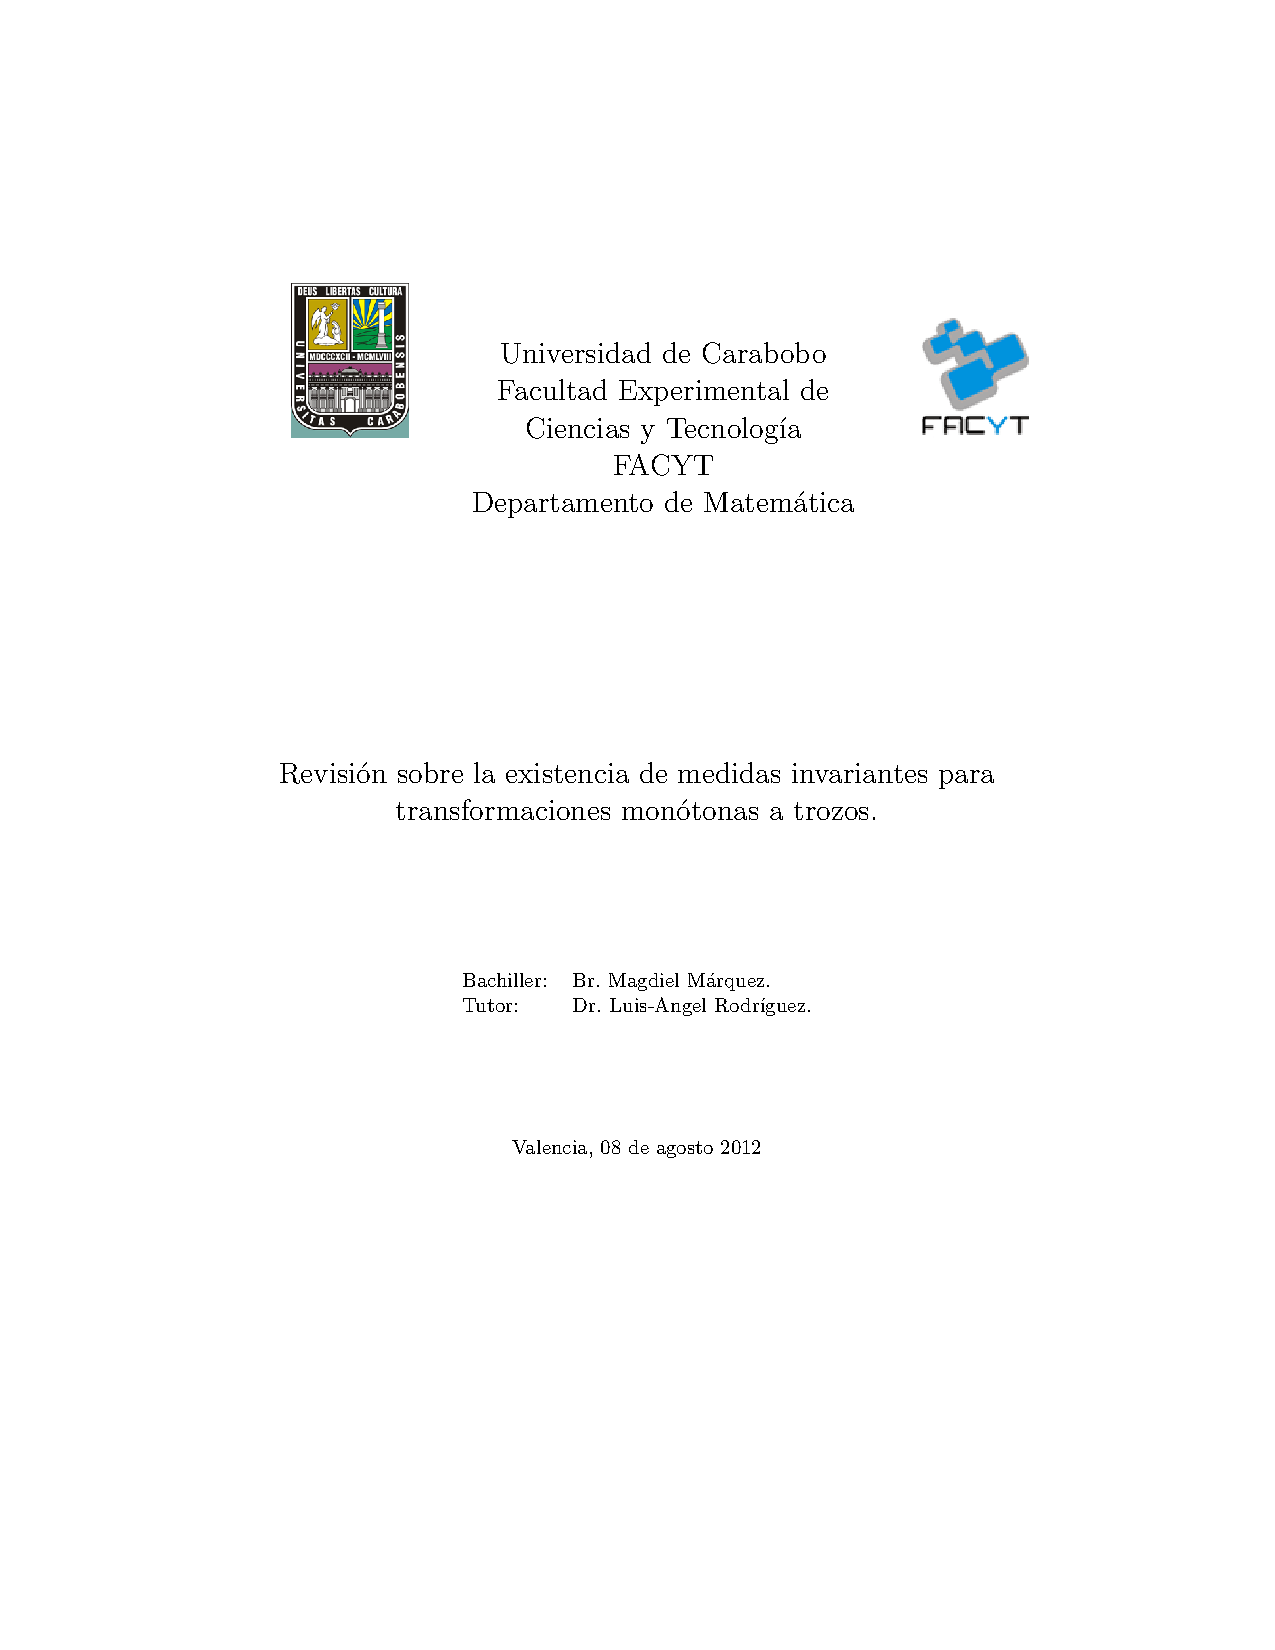
\includegraphics{graficas/tesis.1}
    \end{center}
    \caption{$S(x)=4x(1-x)$\quad para $0\leq x\leq 1$. Se observa como la poblaci�n crece y decrece alrededor de $\alpha$}
    \label{Fig1}
\end{figure}

Al examinar  la poblaci�n de una especie se puede considerar  la variable t como las generaciones de la misma. La cantidad de poblaci�n
de la siguiente generaci�n depender� de la cantidad de la generaci�n anterior mediante la transformaci�n $S$. Debido a lo anterior, el
tiempo se considera discreto sobre las generaciones de la especie. Por lo tanto, para el estudio de la din�mica de la poblaci�n se
considera mediante la siguiente definici�n.

\begin{dfn} (Trayectoria de $x^0$) Es la sucesi�n de estado definidos como
	\begin{equation}
		x^0, S(x^0),\quad  S(S(x^0))=S^2(x^0),\quad S(S(S(x^0)))=S^3(x^0), \ldots \label{trayectorias}
	\end{equation}
    donde $x^0\in[0,1]$  en los  tiempos $1,2,3,\ldots$
\end{dfn}

Al no existir poblaci�n entonces la misma no podr�a variar, as� se esperar�a que al elegir $x^0=0$ la trayectoria no difieran de $0$.
En la Figura (\ref{Fig2})se comprueba dicha observaci�n con la grafica de la trayectoria en forma de serie de tiempo.  Por otra parte,
al elegir $x^1=3/4$ la poblaci�n se mantiene con el paso del tiempo, como se muestra en la Figura (\ref{Fig2}).

\begin{figure}[h]
    \begin{center}
    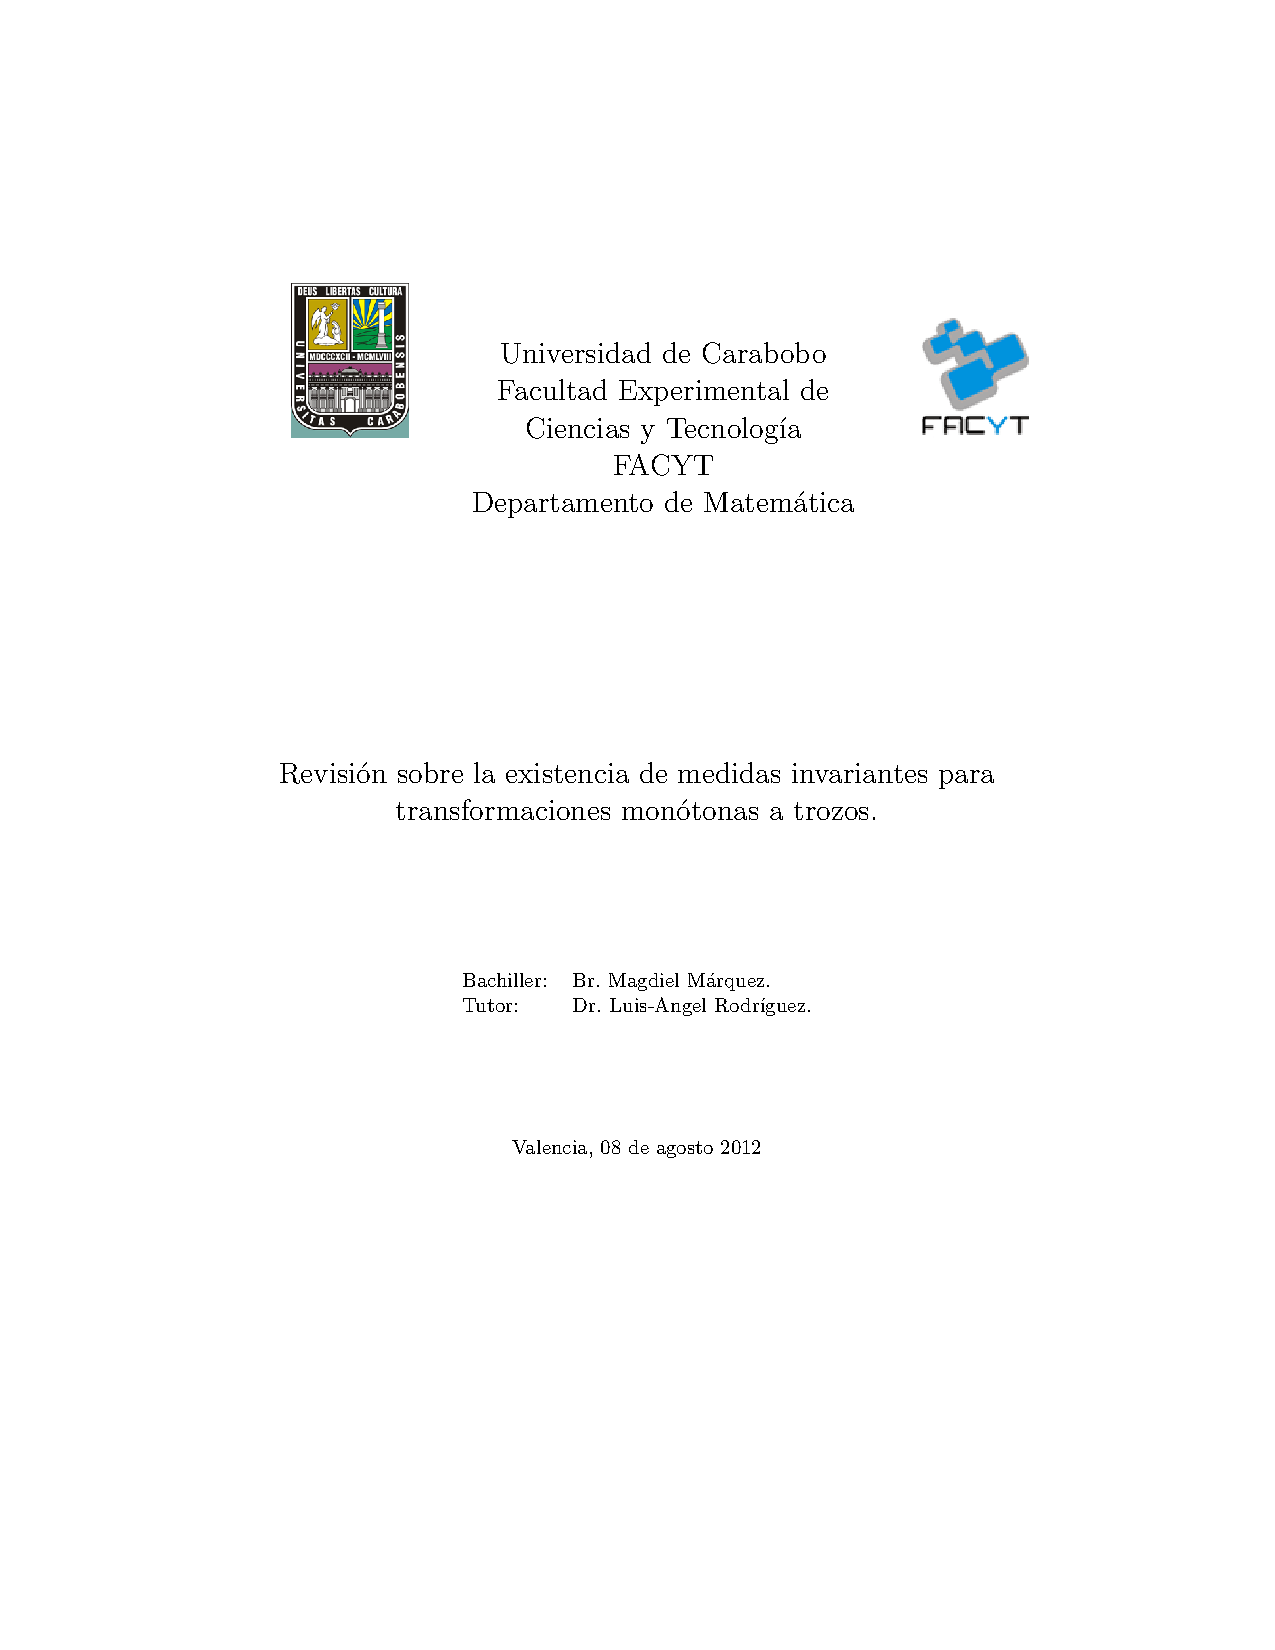
\includegraphics{graficas/tesis.4}\\
    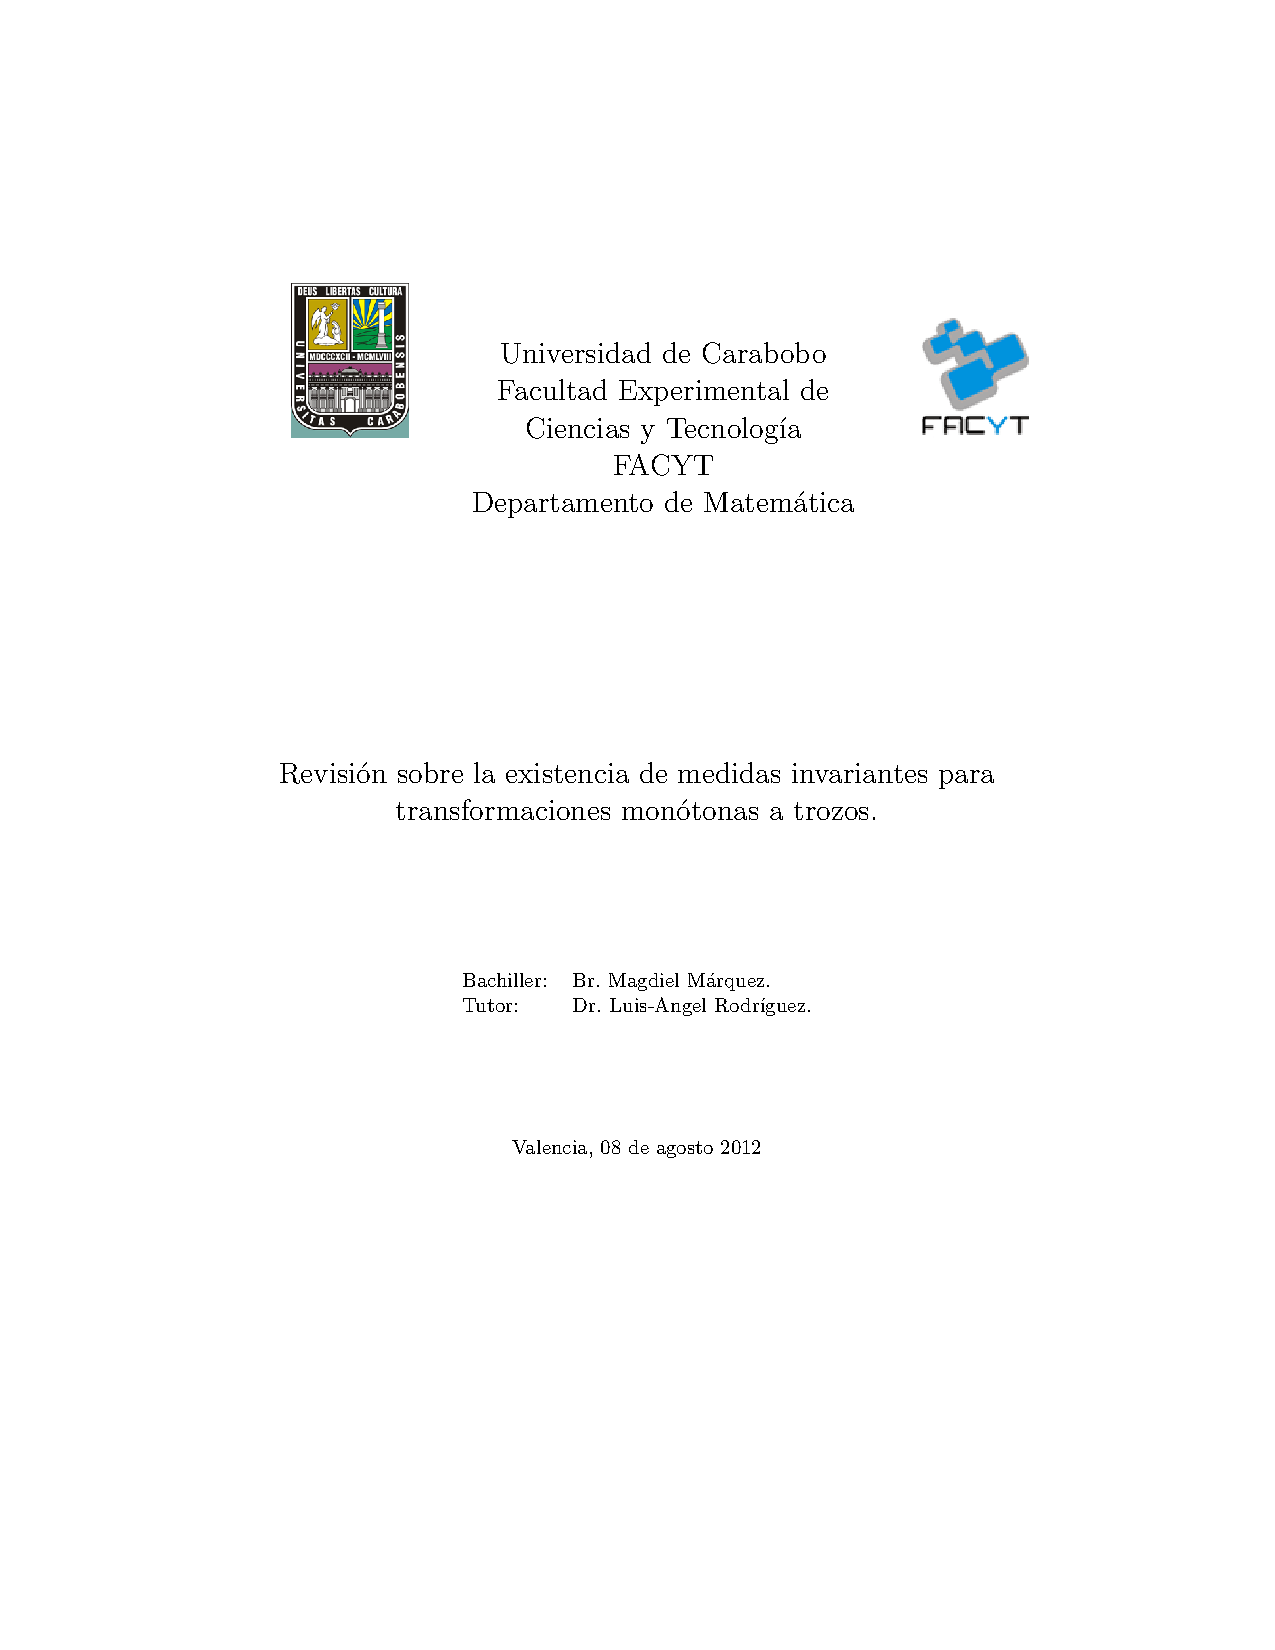
\includegraphics{graficas/tesis.5}
        \begin{picture}(0,0)
        \end{picture}
    \end{center}
    \caption{(Arriba) La trayectoria de $S(x)$ con condici�n inicial $x^0=0$. (Abajo) Trayectoria de $S(x)$ con condici�n inicial $ x^0=\frac{3}{4}$ }
    \label{Fig2}
\end{figure}


Sin embargo, los comportamientos interesantes ocurren alej�ndose de los n�meros racionales entre $[0,1]$ como por ejemplo en $x^0=\pi/10$.
Analizando otro valor inicial cercano a $x^0$ como por ejemplo, $x^1=\pi/10+0.001$. En la Figura (\ref{Fig3}) se presenta las graficas de
la trayectorias. Se observan las trayectorias han variado lo que representar�a un cambio significativo en evoluci�n de la poblaci�n.

\begin{figure}[h]
    \begin{center}
    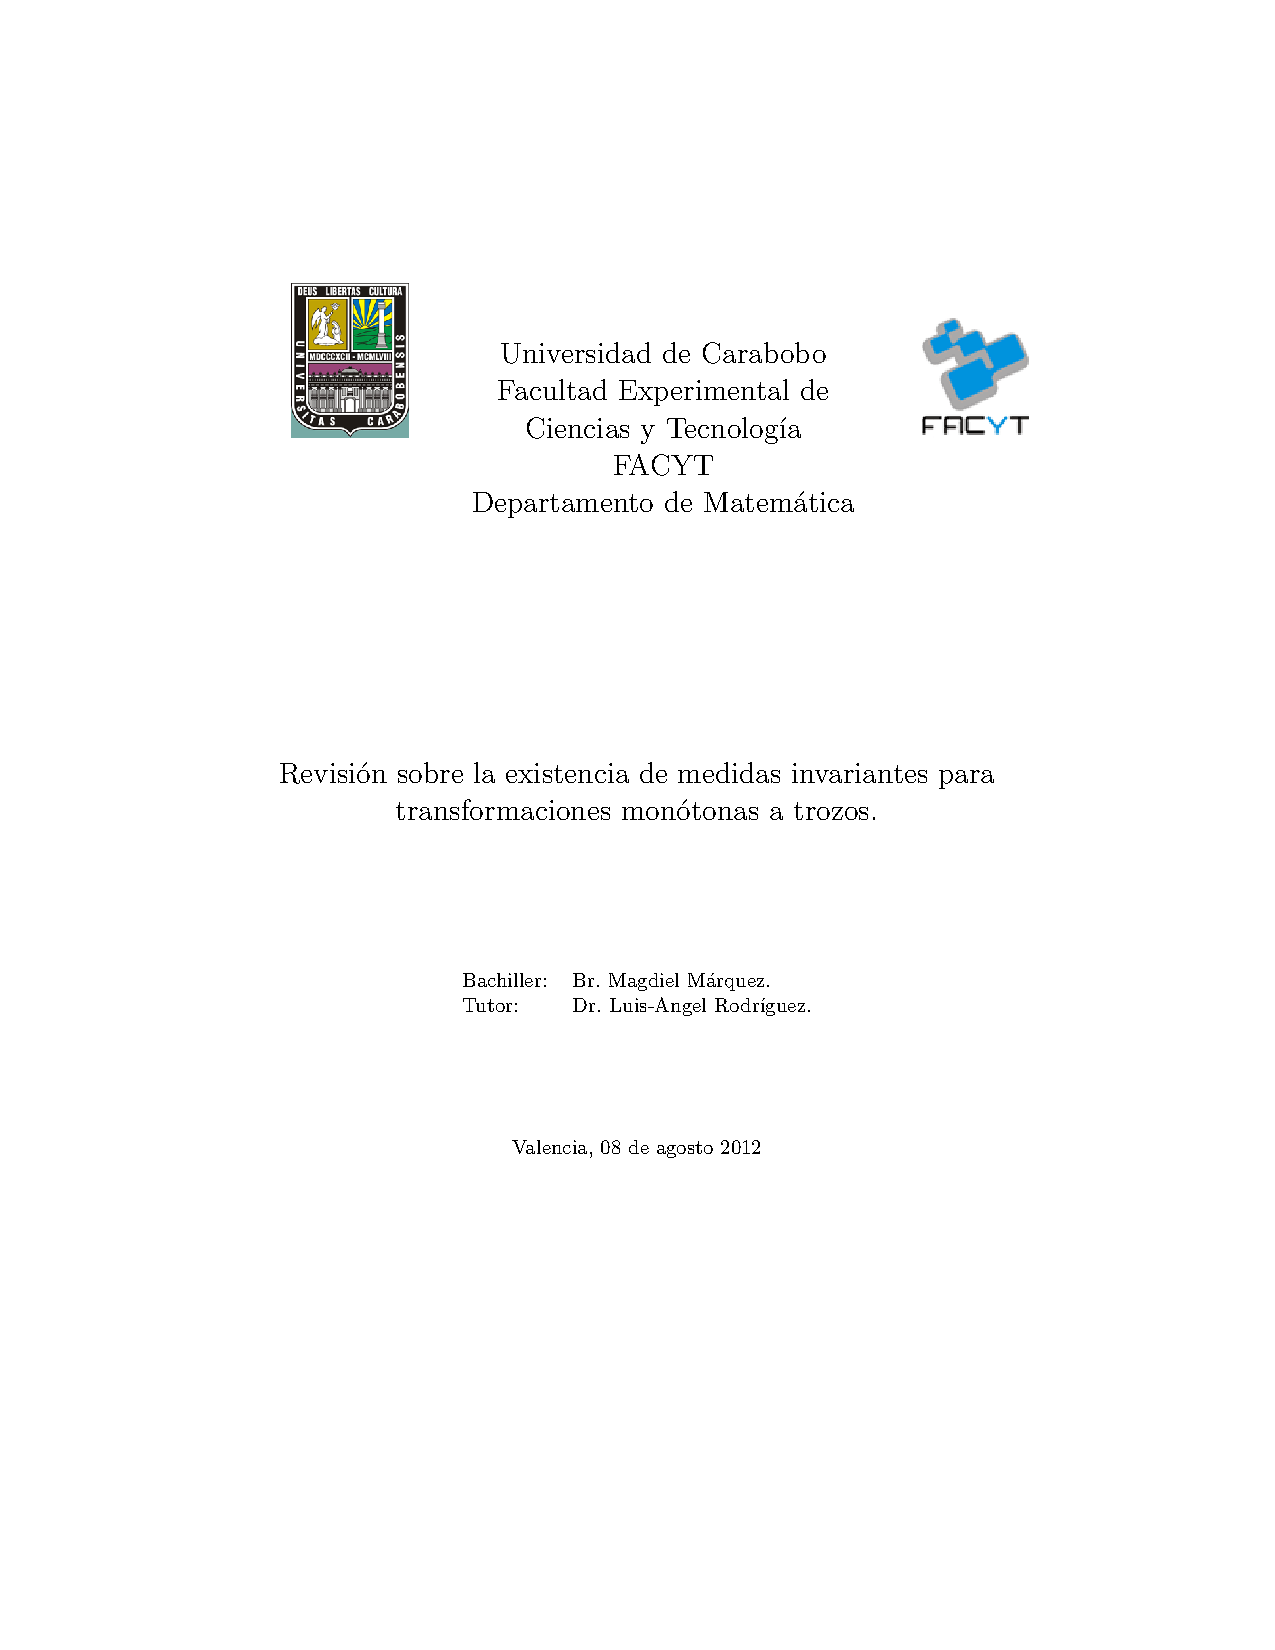
\includegraphics{graficas/tesis.2}\\
    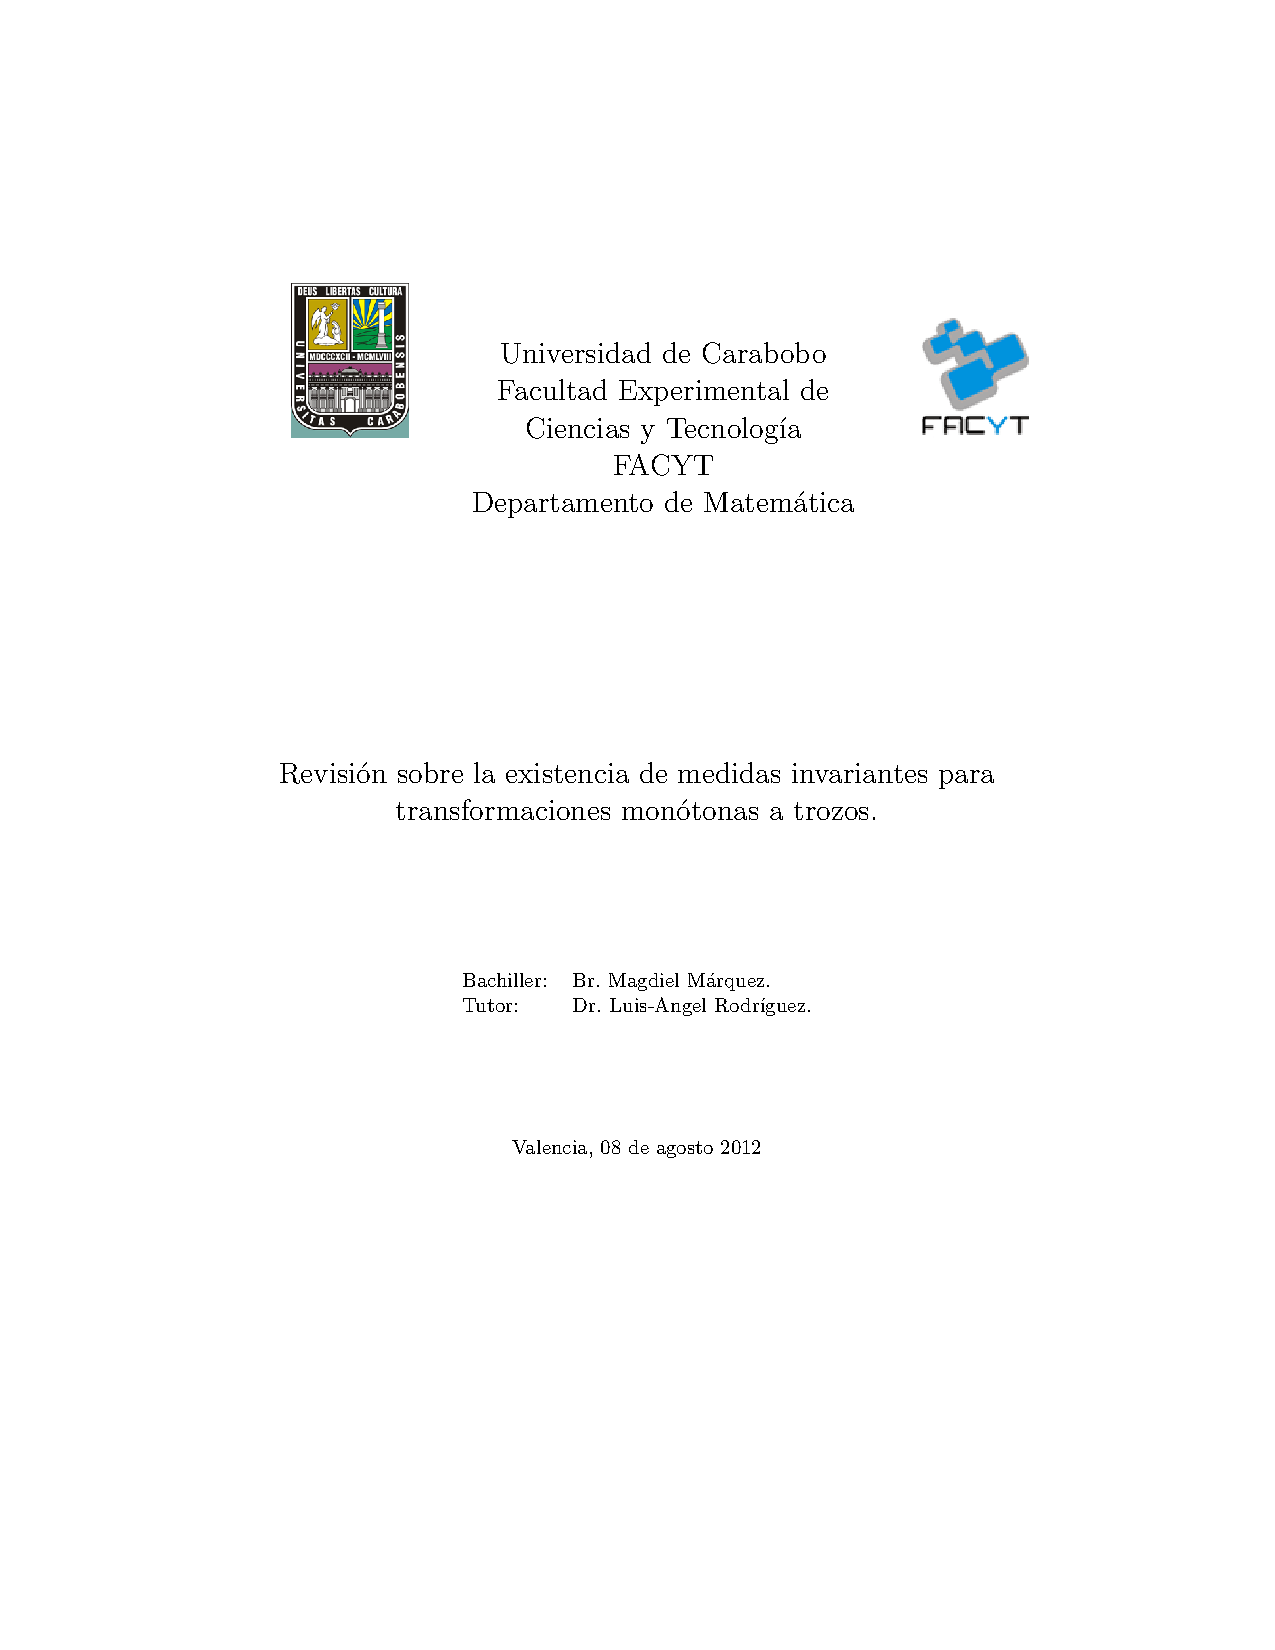
\includegraphics{graficas/tesis.3}
        \begin{picture}(0,0)
        \end{picture}
    \end{center}
    \caption{(Arriba) La trayectoria de $S(x)$ con condici�n inicial $x^0=\pi/10$. (Abajo) Trayectoria de $S(x)$ con condici�n inicial
     $ x^0=\pi/10+0.001$ }
    \label{Fig3}
\end{figure}

Si consideramos

$$X^0=\{x^0(0), S(x^0)=x^0(1), S(S(x^0))=x^0(2),\ldots,x^0(n) \}$$
$$X^1=\{x^1(0), S(x^1)=x^1(1), S(S(x^1))=x^1(2),\ldots,x^1(n) \}$$

Y calculando la norma 2, osea

\begin{align*}
    ||x^0-x^1||&=\sqrt{\sum^{n}_{i=0}{x^0(i)-x^1(i)}}\\
               &=35,909\\
\end{align*}

La norma $||x^0-x^1||$ es mayor que 1 y dado que la diferencia entre $x^0$ y $x^1$ es de una mil�sima.
Lo anterior, indica que la soluci�n es sensible a las condiciones in�ciales.

Se realiza un estudio estad�stico de cada una de las trayectorias. Consideremos el histograma de frecuencia $f_i$;
este se construye de la siguiente forma. Se toma una partici�n $\{I_k\}_k=1,\ldots,n$ del espacio de fases $[0,1]$
y para cada trayectoria definimos las frecuencias

$$f_i=\frac{\sharp\{ x^0(j)\in I_k\}}{N}$$

donde $\sum{f_i}=1$, $N>>n$ y %$[\frac{\imath-1}{n},\frac{\imath}{n})\; \imath=1,\ldots,n$. Por ultimo, se grafica la partici�n $\{ I_k \}$ vs la frecuencia $f_i$.

\begin{table}[h!]
    \begin{tabular}{cc}
          \includegraphics[width=65mm]{anteproyecto/Fig4.jpeg}
          &
          \includegraphics[width=65mm]{anteproyecto/Fig5.jpeg}
    \end{tabular}
    \caption{ (Izquierda) Histograma de frecuencia para $S(x^0)$ con $x^0=\pi/2$.(Derecha) Histograma de frecuencia para $S(x^0)$ con $x^0=\pi/2+0.001$.}
    \label{Fig4}
\end{table}

Se observa simetr�a en el resultado. Las frecuencia son mayores los extremos $0$ y $1$, pero menores pr�ximos al centro en $1/2$.
Repitiendo este proceso para distintos estados in�ciales, o sea, para distintos valores de $x^0$ se obtiene, en general, el mismo resultado.
En resumen: la trayectoria del sistema es muy sensible a peque�os cambios en el estado inicial, pero estos usualmente no producen cambios
considerables en la distribuci�n de estados o frecuencias $f_i $ cuando la trayectoria es grande (o sea $N>>n$).

El estudio de orbitas particulares parece poco fruct�fero, no obstante el an�lisis de las densidades se observa m�s prometedor.
Sin embargo, surgen la varias interrogantes: �C�mo podemos calcular la funci�n de densidad? Y m�s importante a�n, �Existe dicha funci�n
de densidad? �Para cuales condiciones?  En la siguiente secci�n se tratara estos temas.

\subsection{La evoluci�n de las densidades}

Si consideramos que las trayectorias son aleatorias, equidistribuidas e independientes; hip�tesis de la Ley Fuerte de Grandes N�meros nos permite decir que:

$$Lim_{N\rightarrow\infty}{\sum^{N}_{j=1}{1_{\tri_0}(x^0_j)}}=\int_{\tri_0}{f_0(x)\mu(dx)}$$

Sin embargo, por la forma como son generados las trayectorias estas no son independientes por lo que se necesita recurrir a teoremas Erg�dicos.
Los teoremas Erg�dicos pueden pensar se como generalizaciones de las Ley fuerte en caso de no independencia,  en donde:

\begin{dfn}(Funci�n Caracteristicas, $1_\tri (x)$) Se define como:
    \begin{equation}
    1_\tri (x)=
	   \begin{cases}
		  1 & Si\; x\in\tri\\	
          0 & Si\; x \;not\in\tri
        \end{cases}
    \end{equation}
\end{dfn}

Y  $f$ es una funci�n de densidad de $\X$.

Se presentara el operador Perron-Frobenius de forma intuitiva con la finalidad de poder conseguir la funci�n de probabilidad para el ejemplo en estudio.
Inicialmente, se supone que tenemos la transformaci�n $S:[0,1]\cir$ (una forma abreviada de decir $S[0,1]$ en si misma). Se recoge un
gran n�mero $N$ de estados in�ciales

$$x_1^0, x_2^0, x_3^0,\ldots, x_N^0$$

Para cada uno de los estados se le aplica la transformaci�n  S, obteniendo  as� $N$ nuevos estados denotados por

$$x_1^1=S(x_1^0), x_2^1=S(x_2^0), \ldots, x_N^1=S(x_n^0)$$

En t�rminos generales, decimos que una funci�n $f_0(x)$ es una funci�n de densidad para el valor inicial
$x_1^0, x_2^0, x_3^0,\ldots, x_N^0$ si, para cada intervalo (no tan peque�o) $\tri_0\subset[0,1]$ tenemos

\begin{equation}
    \int_{\tri_0}{f_0(\mu)d\mu}\simeq\frac{1}{N}\sum_{j=1}^{N}{1_{\tri_0}(x_j^0)}
\end{equation}

Similarmente, la funci�n densidad $f_1(x)$ para los estados $x_1^1, x_2^1, x_3^1,\ldots, x_N^1$ la satisface por $\tri\subset[0,1]$

\begin{equation}
    \int_{\tri}{f_1(\mu)d\mu}\simeq\frac{1}{N}\sum_{j=1}^{N}{1_\tri(x_j^1)}
\end{equation}

Se quiere encontrar la relaci�n entre $f_1$ y $f_2$. Para hacer esto es necesario introducir la noci�n de imagen inversa.

\begin{dfn}(Imagen inversa de $S$, $S^{-1}(\tri)$) Es el conjunto de todos los puntos que estan en $\tri$ luego la aplicaci�n de S, o
$$S^{-1}(\tri)=\{x:S(x)\in\tri\}$$
\end{dfn}

Observe que para cualquier $\tri\subset[0,1]$ se tiene

$$x^1_j\in\tri\qquad sii\, x_1^0\in S^{-1}(\tri)$$

En consecuencia, se deducir la �til relaci�n

\begin{equation}
    1_\tri(S(x))=1_{S^{-1}(x)}(x)
\end{equation}

Se puede reescribir la ecuaci�n como

\begin{equation}
    \int_\tri{f_1(\mu)d\mu}\simeq\frac{1}{N}\sum_{j=1}^N{1_{S^{-1}(\tri)}(x_j^0)}
\end{equation}

Siendo $\tri_0$ y $\tri$ ha sido arbitraria hasta este punto, simplemente, escogemos $\tri_0=S^{-1}(\tri)$. Con esta opci�n la ecuaciones %%% son iguales y por lo tanto

\begin{equation}
    \int_\tri{f_1(\mu)d\mu}=\int_{S^{-1}(\tri)}{f_0(\mu)d\mu} \label{rela}
\end{equation}

Esta ecuaci�n nos entrega la relaci�n que existe entre las funciones densidad $f_0$ y $f_1$ , y nos dice como
cambia la densidad para los estados iniciales al aplicarles la transformacion $S$ ,es decir , nos dice como la
funcion densidad $f_0$ es cambiada a una nueva funcion $f_1$ al aplicar la transformacion $S$.

Ahora bien: si $\tri$ es un intervalo , digamos $\tri=[a,x]$ , entonces podemos obtener una
representacion explicita para $f_1$ .En este caso , la ecuacion ~(\ref{rela})se transforma en :


$$\int_a^x{f_1(\mu)d\mu}=\int_{S^{-1}([a,x])}{f_0(\mu)d\mu}$$

derivando con respecto a $x$ tenemos

\begin{equation}
    f_1(x)=\frac{d}{dx}\int_{S^{-1}([a,x])}{f_0(\mu)d\mu} \label{rela2}
\end{equation}

Ahora es claro que $f_1$ depender� de $f_0$.Esta dependencia se indica usualmente escribiendo $f_1=\Pm f_0$
y entonces podemos escribir la ecuaci�n ~(\ref{rela2}) como :

\begin{equation}
    Pf(x)=\frac{d}{dx}\int_{S^{-1}([a,x])}{f(\mu)d\mu}
\end{equation}

Este operador se le conoce como el nombre de Perron-Frobenius. Para ilustrar el uso de esta formula el resultado en el ejemplo ya estudiado.
Se procede a calcular la regi�n de la inversa de S. Esto se puede hacer despejado la funcion con respecto a y

\begin{align*}
    4x(1-x)&=y         && \text{se despeja x} \\
\intertext{Operando la expresi�n resulta as�}
          x&=\frac{2\mp 2\sqrt{(1-y)}}{4} && \\%\text{elevando al cuadrado}\\
\end{align*}

Se obtiene la region de integraci�n.

$$S^{-1}([0,x])=[0,\frac{1}{2}-\frac{1}{2}\sqrt{1-x}]\cup[\frac{1}{2}+\frac{1}{2}\sqrt{1-x},1]$$

Sustituyendo en \ref{rela2} se obtiene

\begin{align*}
    \Pm f(x)&=\frac{d}{dx}\int_{[0,\frac{1}{2}-\frac{1}{2}\sqrt{1-x}]\cup[\frac{1}{2}+\frac{1}{2}\sqrt{1-x},1]}{f(u)du}\\
            &=\frac{d}{dx}\int^{\frac{1}{2}-\frac{1}{2}\sqrt{1-x}}_0{f(u)du}+\frac{d}{du}\int^1_{\frac{1}{2}+\frac{1}{2}\sqrt{1-x}}{f(u)du}\\
%\intertext{Suponiendo que \frac{dF}{dx}=f}
            &=\frac{d}{dx}F\Big(\frac{1}{2}-\frac{1}{2}\sqrt{1-x}\Big)
            -\frac{d}{dx}F(0)+\frac{d}{dx}F(1)-\frac{d}{dx}F\Big(\frac{1}{2}+\frac{1}{2}\sqrt{1-x}\Big)\\
            &=\frac{1}{4\sqrt{1-x}}\{f(\frac{1}{2}-\frac{1}{2}\sqrt{1-x})+f(\frac{1}{2}+\frac{1}{2}\sqrt{1-x})\}
\end{align*}

Supongamos que $f(x)=1$ para $x\in [0,1]$. Entonces la formula anterior se simplifica como

\begin{equation}
    \Pm f(x)=\frac{1}{2\sqrt{1-x}}
\end{equation}

Ahora se sustituye la expresion $\Pm$ por $f$ y podemos calcular nuevamente $\Pm(\Pm f(x))=\Pm^2f(x)$. En la investigaci�n se mostr� que para
este ejemplo en especifico la sucesi�n de densidades converge a una densidad limite dada por:

\begin{equation}
    f_*(x)=\frac{1}{\pi\sqrt{1-x}}
    \label{limite}
\end{equation}

Con lo cual, se consigue el c�lculo de la densidad de probabilidad, aunque las condiciones para la existencia no han sido 
tratadas. El \emph{estudio de la existencia} ser� el tema a desarrollar en la presente investigaci�n. 
As� mismo, como las razones que justifican el paso al l�mite
de  (~\ref{limite}). Como profundizar en las propiedades del operador de Perron-Frobenius.

Recapitulando, debido a la sensibilidad a las condiciones in�ciales de algunas funciones se opta en tratar un
 problema determinista como un problema
estoc�stico. Enti�ndase como problema determinista hallar el comportamiento asint�tico de la soluci�n de una ecuaci�n diferencial. As� mismo, como
problema estoc�stico el de encontrar  la funci�n de probabilidad que siguen las trayectorias. Se mostro como
 el operador de Perron-Frobenius colabora en
proporcionado un m�todo recursivo para encontrar una sucesi�n que converge a la funci�n de probabilidad deseada. Aunque, no quedo claro el paso al
l�mite de la sucesi�n anterior. Menos aun, las hip�tesis y razonamiento que justifique el procedimiento anterior. Estos temas ser�n tratado en del
desarrollo de la investigaci�n.

%\section{Objetivos}

\subsection{Objetivo General}
    Estudiar condiciones para la existencia de medidas invariantes de sistemas din�micos reales.
\subsection{Objetivos Espec�ficos}
    \begin{itemize}
        \item Estudiar algunos elementos del operador de Markov.
        \item Estudiar el operador de Frobenius-Perron.
        \item Demostrar la existencia de medidas invariantes absolutamente continuas.
        \item Experimentar en el computador algunos ejemplos de densidades invariantes para sistema din�micos reales.
    \end{itemize}

\section{Cronograma de Actividades}
    En esta secci�n, se expondr� las actividades ha ejecutar para la realizaci�n del Trabajo Especial de Grado, as� como, el cronograma de actividades para la elaboraci�n del mismo.
\subsection{Actividades a realizar}
    \begin{enumerate}
        \item Revisi�n de las notas ``Notas para un curso de teoria erg�dica'' de Fernando J. S�nchez S.
        \item Revisi�n del libro ``Probabilistic properties of deterministic systems''  de A. Lasota \& Michael C. Mackey
        \item Realizaci�n de los resultados del art�culo ``On the existence of invariant measures for piecewise monotonic transformations'',
         de A. Lasota y James A. Yorke.
        \item Realizaci�n de ejemplos sobre densidades invariantes para sistema din�micos reales.
        \item Redacci�n del Trabajo Especial de Grado.
    \end{enumerate}


\begin{table}
\begin{center}
        \begin{tabular}{|c|c|c|c|c|c|}
             \hline
             \backslashbox{Act}{Sem}     & 1 & 2 & 3 & 4 & 5 \\
             \hline
             \backslashbox{13-08}{17-08} & X &   &   &   & X \\
             \hline
             \backslashbox{20-08}{24-08} & X &   &   &   & X \\
             \hline
             \backslashbox{27-08}{31-08} &   & X &   &   & X \\
             \hline
             \backslashbox{03-09}{07-09} &   & X &   &   & X \\
             \hline
             \backslashbox{10-09}{14-09} &   &   & X &   & X \\
             \hline
             \backslashbox{17-09}{21-09} &   &   & X &   & X \\
             \hline
             \backslashbox{24-09}{28-09} &   &   &   & X & X \\
             \hline
             \backslashbox{01-10}{05-10} &   &   &   & X & X \\
             \hline
        \end{tabular}
\end{center}
\caption{Diagrama de Grantt}
\end{table}

%%%%%%%%%%%%%%%%%%%%%%%%%%%%%%%%%%%%%

\tableofcontents
\section{Introduccion}
Sea $(\X, \A,\mu)$ un espacio de medida. Una medida se llama invariante bajo una transformaci\'on $S:\X\rightarrow\X$ si
$\mu(A)=\mu(S^{-1}(A))$ para $A\in\A$
Se puede observar que para una funci\'on $f:[0,1]\rightarrow[0,1]$ no existe un medida invariante absolutamente
continua, si la grafica de $f$ es muy plana. Por ejemplo: para la transformaci\'on $f(x)=rx (mod 1) $ con $|r|<1$ una medida invariante no existe.

En 1957 S. Ulam propuso el problema de la existencia de medidas invariantes absolutamente continuas
para funciones definidas por funciones suficientemente simples\footnote{Ejemplo: funciones lineales a trozos o poligonales}
donde el gr\'afico no corte la l\'inea $y=x$ con una pendiente de valor absoluto menor que 1. La respuesta  literal de
esta pregunta es negativa. Se puede ilustrar, que para la siguiente transformaci\'on

$$f(x)=\begin{cases}
		 1-2x     & 0\leq x\leq\frac{5}{12}\\	
         (2-2x)/7 & \frac{5}{12}< x\leq 1
        \end{cases}$$

No existe una medida invariante absolutamente continua. Note que esta transformaci\'on cruza la
l\'inea $y=x$ en el punto $x=\frac{1}{3}$ con pendiente $f'(x)=-2$.

Muchos resultados en relaci\'on de la existencia de medidas absolutamente contin\'uas para ciertas clases de
transformaciones del  intervalo unitario en si mismo han sido proporcionadas (A. R\'enyi, Parry, Krzyzewski/Szlenk).
Sin embargo, se puede se\~nalar que el mejor resultado en esta direcci\'on fue obtenido por A. Lasota y J. Yorke

\begin{teo} Sea $S:[0,1]\rightarrow[0,1]$ una funci\'on a trozos de clases $C^2$ que satisfaga la condici\'on
$$\inf_{x\in[0,1]}|\frac{d}{dx}f(x)|>1$$
Entonces existe una medida invariante absolutamente continua sobre $f$
\end{teo}

La metodolog\'ia usada por Lasota/Yorke en la demostraci\'on difiere  de los trabajos antes mencionados. En primer lugar se
uso el hecho de que operador de  Perron-Frobenius correspondiente a la transformaci\'on  tiene la propiedad de contracci\'on
en la variaci\'on de la funci\'on.  Luego prueba que cierta sucesi\'on es relativamente compacta, as\'i se cumplen en la
hip\'otesis del teorema de Mazur.

Esto garantiza, que el promedio de las orbitas convergen fuertemente a una funci\'on limite, por medio  al uso de teorema
de Kakutani-Yosida.  Repitiendo este proceso se consigue una familia de funciones que acotan a la variaci\'on del operador
de Perron-Frobenius. Para finalizar, usando el principio de selecci\'on de Helly se puede conseguir una sucesi\'on de funciones,
que convergen a una funci\'on de variaci\'on finita.

El objetivo del presente trabajo es aclarar lo detalles de la  presente demostraci\'on con lo cual se presentar\'a en el primer
cap\'itulo una introducci\'on intuitiva a los s\'istemas din\'amicos, caos y el operador de Perron-Frobenius. En el siguiente
cap\'itulo se analizar\'a en detalle el operador de Perron-Frobenius. En el tercer cap\'itulo,
se presenta la noci\'on de ergodicidad junto con otros niveles de irregularidades. El cuarto cap\'itulo est\'a dedicado a estudio
del los teoremas de Mazur, Kakutani-Yosida, asi tambi\'en  como del Principio de Helly.

Finalmente, se presenta el quinto cap\'itulo se probar\'a el teorema de Lasota-Yorke junto con un contra ejemplo. Los ap\'endices expuestos tratan
de unas nociones b\'asicas de s\'stemas din\'amicos y de teor\'ia de la medida necesaria para el desarrollo  de los temas tratados.


\chapter{Sistemas Din�micos}

Los astros han sido del inter�s humano desde hace varios siglos. No obstante, La presencia de ecuaciones diferenciales no-lineales
ha dificultado el estudio de los mismos. La din�mica, el movimiento, de 3 cuerpos celestes originado por la interacci�n de gravitatoria de los mismos;
se le conoce como \textit{el problema de los 3 cuerpos}. A finales del siglo XIX, Henri Poicar� (1854-1912) desarroll� el an�lisis
cualitativo de las ecuaciones diferenciales estudiando el problema de los 3 cuerpos. De esta forma surgen los Sistemas Din�micos.

El objetivo de los sistemas din�micos es el estudio del comportamiento asint�tico o a largo plazo de un sistema que depende del tiempo.
Por ejemplo, si consideramos la cantidad de poblaci�n de una especie su comportamiento asint�tico nos proporciona informaci�n �til sobre la
supervivencia o extinci�n de dicha especie. Como puede advertirse,  los Sistemas Din�micos tiene asida la idea de movimiento o cambio con
respecto al tiempo.

Esta idea se representa con  la noci�n de grupo de acci�n; la cual ser� presentada en el ap�ndice~\ref{cha:ApeA}.
Los grupos de acci�n aunque son amplios e interesante te�ricamente hablando, aunque no responden al objetivo fundamental de los
sistemas din�micos anteriormente discutidos.Como consecuencia, se requiere tener cierta estructura sobre el conjunto $\X$, as� como
restricciones sobre $S$. Existe tres ramas principales:

\begin{description}
    \item[Din�mica Diferencial] $\X$ una variedad diferenciable y $S$ un difeomorfismo.
    \item[Din�mica Topol�gica]  $\X$ un espacio topol�gico y $S$ un homeomorfismo.
    \item[Teor�a Erg�dica] $\X$ un espacio de medida y una medida invariante sobre $S$.
\end{description}

El desarrollo de la investigaci�n se fundamentar� en el estudio de algunos elementos de la teor�a erg�dica. Especialmente, aquellos
aspectos estrechamente vinculados al estudio de propiedades estad�sticas \footnote{aleatorio o estoc�stico} de los sistemas din�micos.

Sin embargo, se coment� que los sistemas din�micos surgen el estudio cualitativo de las ecuaciones diferenciales; �rea de
investigaci�n propiamente deterministica. Entonces, �C�mo se fundamentar� la investigaci�n  en algunos elementos de teor�a erg�dica
vinculados con propiedades estoc�sticas?. La conexi�n entre sistemas determin�sticos y estoc�sticos se analizar� en la siguiente secci�n
mediante un ejemplo.

\section{Ejemplo ilustrativo}

La tasa de crecimiento en la poblaci�n de una especie es proporcional a la poblaci�n  real en cualquier instante dado. Si $x$ representa
la cantidad de espec�menes en cualquier instante dado y $t$ las unidades de tiempo, entonces

$$\frac{dx}{dt}=\alpha x$$

representa la din�mica de una poblaci�n. Donde $\alpha$ es una contante; si $\alpha>0$ se tiene una ley de crecimiento natural y si $\alpha<0$
se tiene una ley de decrecimiento natural.

Sin embargo, al comparar dicho modelo con la evidencia experimental se comprob� que no se ajustaba a la realidad. Ninguna poblaci�n
puede crecer indefinidamente a una tasa constante; ya sea por limitaciones de espacio, recursos, entre otros. Por lo tanto, es realista suponer
que el medio solo puede sostener de manera estable un m�ximo $\alpha$ de poblaci�n, de modo que si

\begin{description}
    \item[$x(t)>\alpha$,] la tasa ser�a negativa y la poblaci�n decrecer�a acercandose a $\alpha$.
    \item[$x(t)=\alpha$,] la tasa ser�a nula y, por lo tanto, la poblaci�n constante.
    \item[$x(t)<\alpha$,] la tasa ser�a positiva, creciendo entonces la poblaci�n, aunque m�s lentamente cuando m�s proxima est� del valor de $\alpha$.
\end{description}

De lo dicho previamente se puede reformular la ecuaci�n que representa la din�mica de una poblaci�n, la ecuaci�n log�stica, como

$$x'=\alpha x(1-x)\;\footnote{donde x' representa clasicamente la derivada de x con respecto del tiempo}$$

Por consiguiente, podemos considera la siguiente definici�n

\begin{dfn}[Familia Log�stica] Es la transformaci�n definida como:
	\begin{equation}\label{logistica}
        S(x)=\alpha x(1-x)\qquad para\; 0\leq x\leq 1
	\end{equation}
\end{dfn}

Se supondra $\alpha=4$. La transformaci�n est� definida en $[0,1]$ en s� misma, dicho de otro modo, el  \emph{estado} o
\emph{fase}  \emph{del espacio} es $[0,1]$. La gr�fica de la transformaci�n se muestra en la siguiente Figura \ref{Glogistica}

\begin{figure}[ht!]
    \begin{center}
        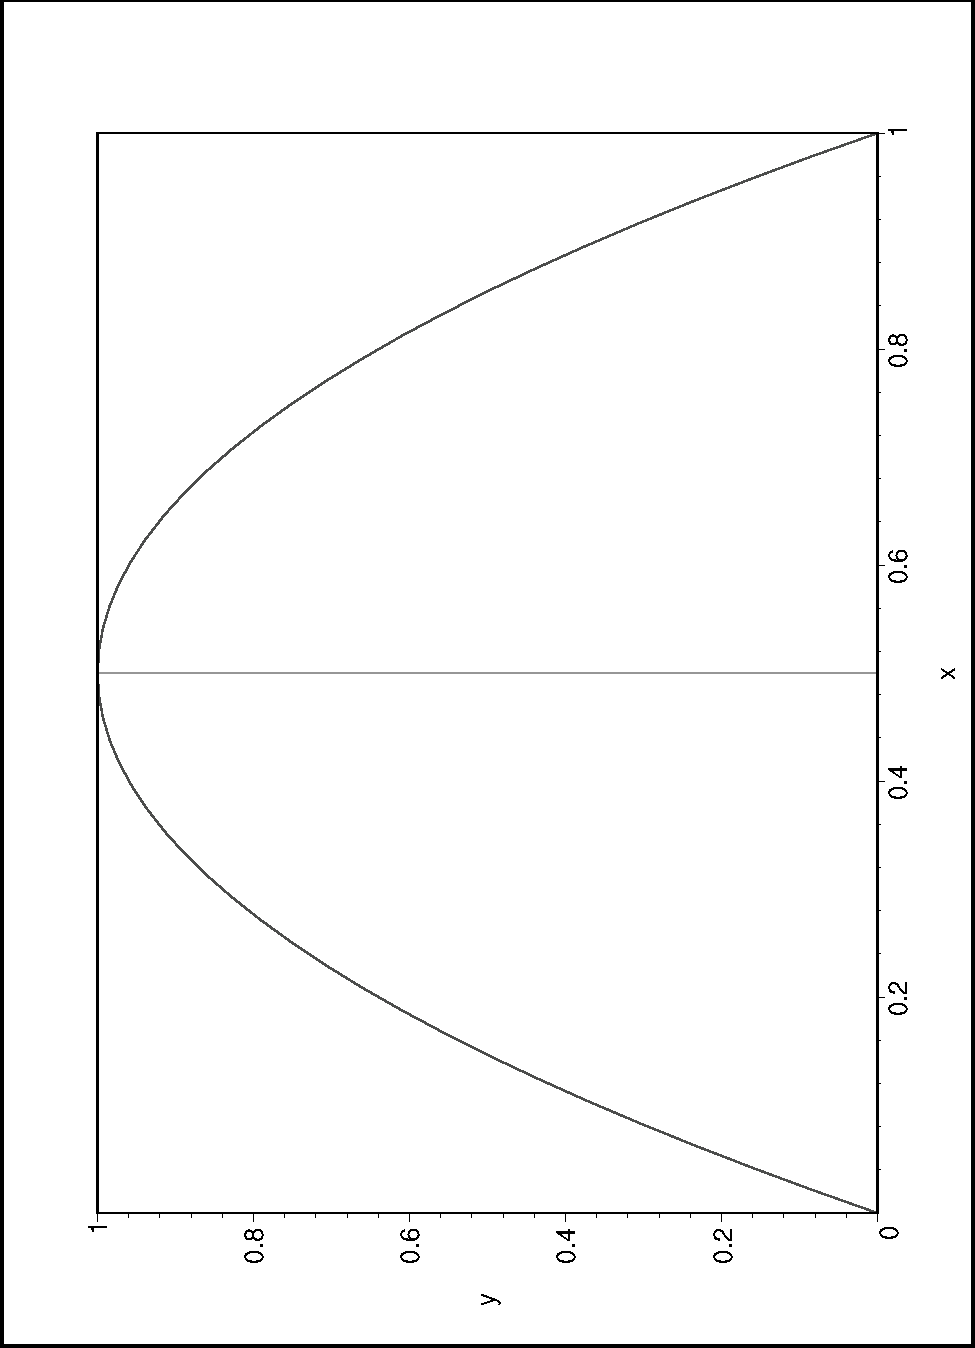
\includegraphics[angle=-90,scale=0.4]{graficas/log}
    \end{center}
    \caption{Gr�fica $S(x)=4x(1-x)$\quad para $0\leq x\leq 1$. Se observa como la poblaci�n crece y decrece alrededor de $\alpha$}
    \label{Glogistica}
\end{figure}

Al examinar  la poblaci�n de una especie, se puede considerar  la variable t como las generaciones de la misma. La cantidad de poblaci�n
de la siguiente generaci�n depender� de la cantidad de poblaci�n actual mediante la transformaci�n $S$. Debido a lo anterior, el
tiempo se considera discreto sobre las generaciones de la especie. Por lo tanto, para el estudio de la din�mica de la poblaci�n se
considera mediante la siguiente definici�n.

\begin{dfn} (Trayectoria\footnote{tambien llamada orbita de $x^0$} de $x^0$) Es la sucesi�n de estado definidos como
	\begin{equation}
		x^0, S(x^0),\quad  S(S(x^0))=S^2(x^0),\quad S(S(S(x^0)))=S^3(x^0), \ldots
    \end{equation}
    donde $x^0\in[0,1]$  en los  tiempos $1,2,3,\ldots$
\end{dfn}

Al no existir poblaci�n entonces la misma no podr�a variar, as� se esperar�a que al elegir $x^0=0$ la trayectoria no difieran de $0$.
La primera parte de la Figura \ref{OFlogistica} se comprueba dicha observaci�n con la grafica de la trayectoria en forma de serie de tiempo.
Por otra parte, al elegir $x^1=\frac{3}{4}$ la poblaci�n se mantiene con el paso del tiempo, como se muestra en la ultima Figura \ref{OFlogistica}.

\begin{figure}
    \begin{center}
        \subfloat[xo]{%\label{f:xo}
            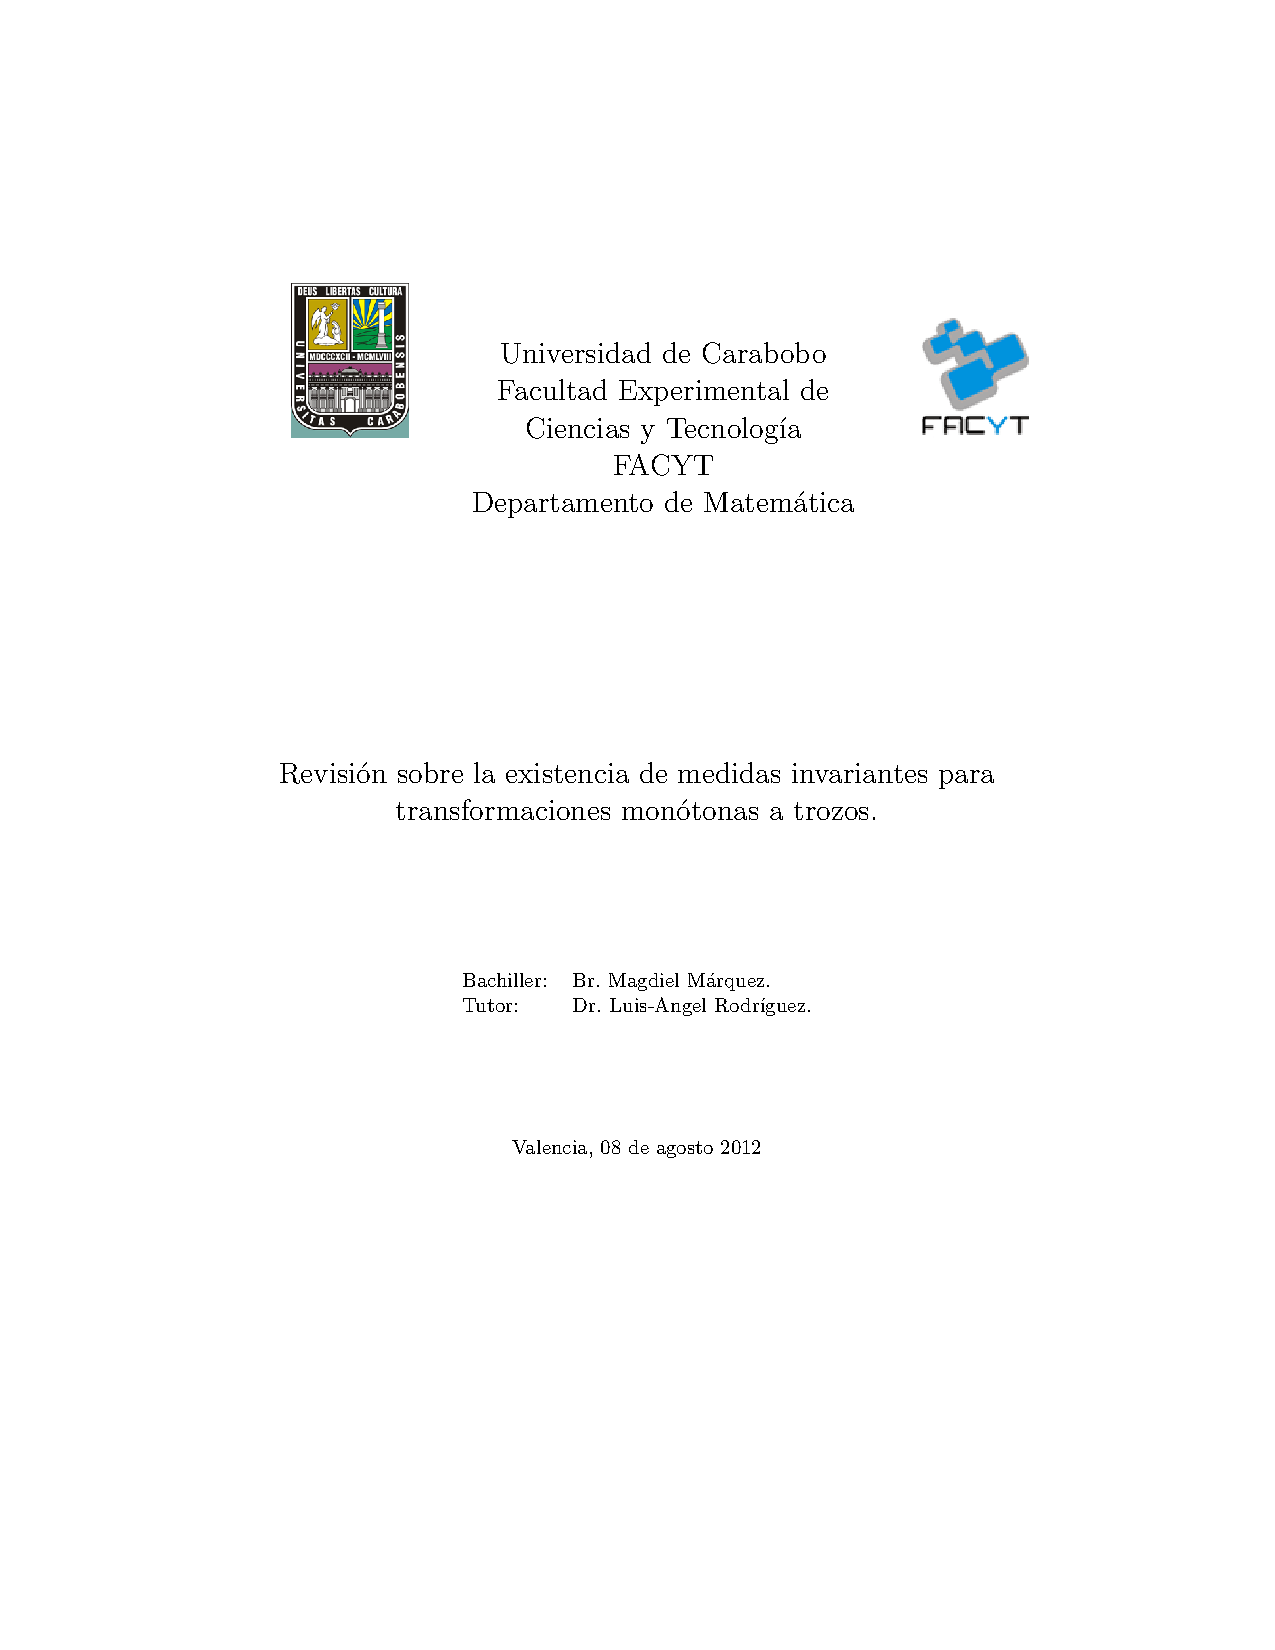
\includegraphics{graficas/tesis.4}}\\
        \subfloat[xm]{%\label{\f:xm}
            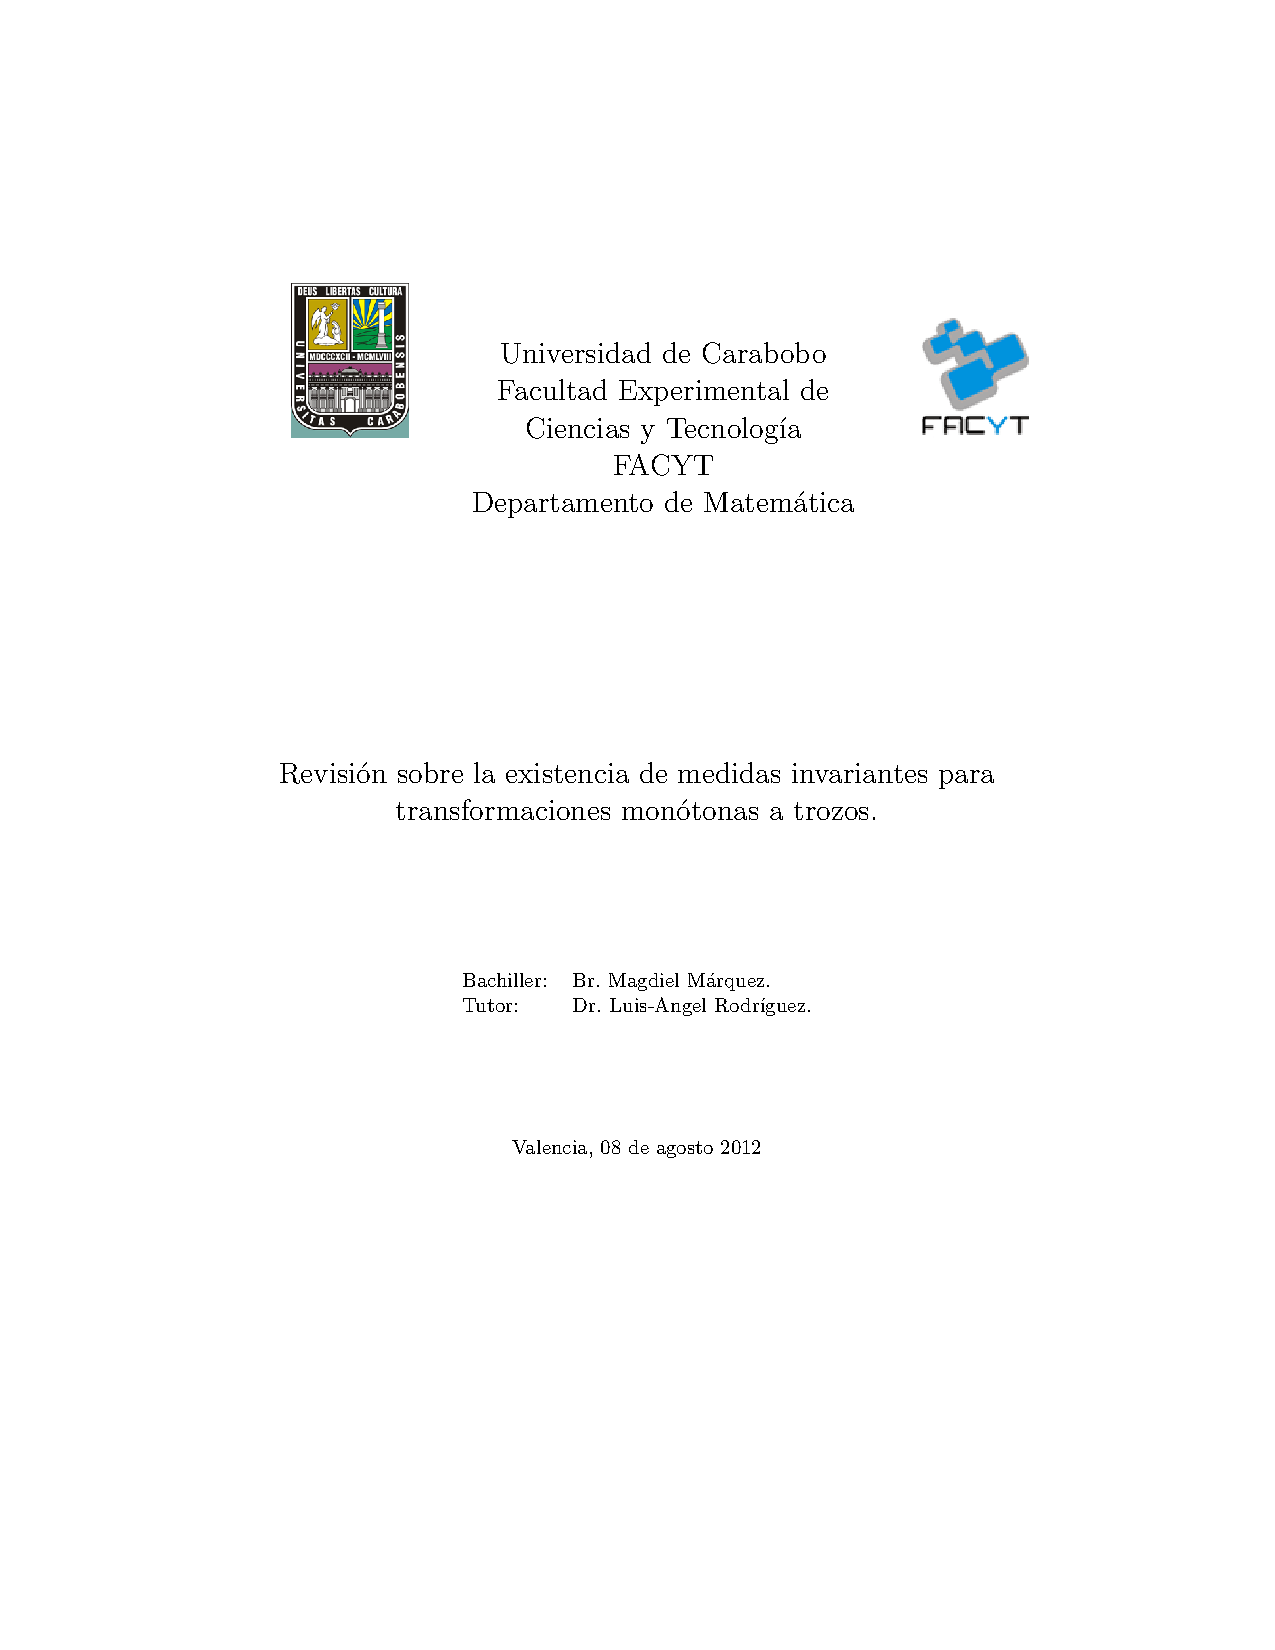
\includegraphics{graficas/tesis.5}}
    \end{center}
    \caption{(Arriba) La trayectoria de $S(x)$ con condici�n inicial $x^0=0$.
     (Abajo) Trayectoria de $S(x)$ con condici�n inicial $ x^1=\frac{3}{4}$ }
     \label{OFlogistica}
\end{figure}

\begin{figure}
    \begin{center}
    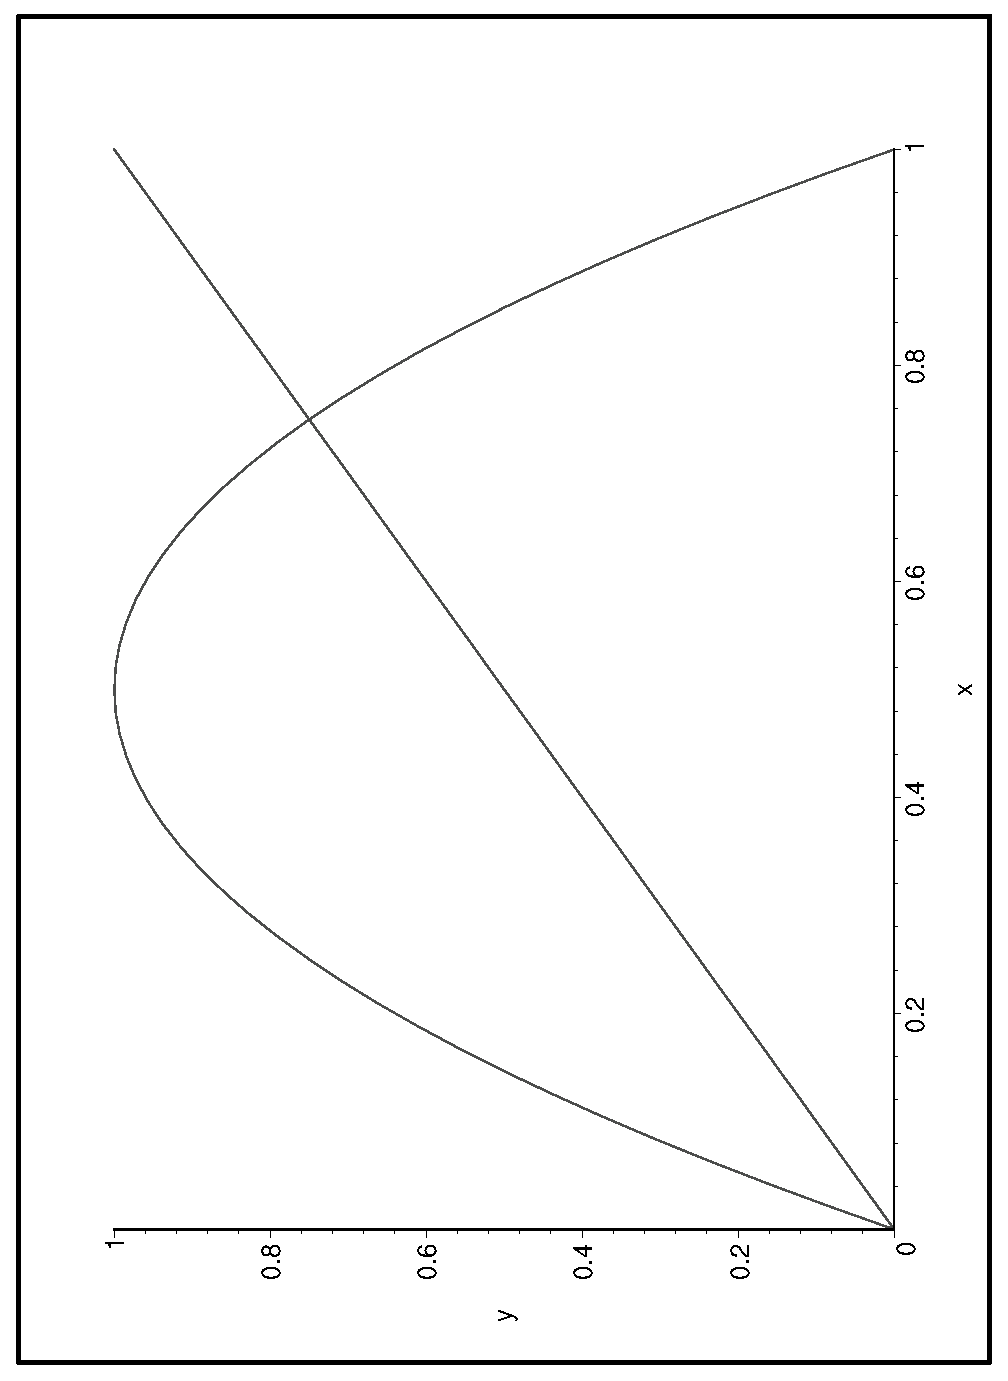
\includegraphics[angle=-90,scale=0.4]{graficas/loi}
    \end{center}
    \caption{Gr�fica $S(x)=4x(1-x)$ e $y=x$.Ambas se interceptan en los puntos $x=0$ y $x=\frac{3}{4}X$}
    \label{OGlogistica}
\end{figure}

Ahora en ambos puntos $0$ y $\frac{3}{4}$ son interesantes para la funci�n log�stica. En la Figura \ref{OGlogistica} se muestra
la funci�n log�stica y la identidad. Ambas funciones se cortan en $0$ y $\frac{3}{4}$; cuando se cortan la orbitas de
estos puntos no var�an. Esto motiva la siguiente definici�n

\begin{dfn}[Puntos fijos] Son los puntos $x$ que cumple
    \begin{equation}
        T(x)=x
    \end{equation}
\end{dfn}

Sin embargo, comportamientos interesantes ocurren alej�ndose de los n�meros racionales entre $[0,1]$ como por ejemplo en $x^0=\pi/10$.
Analizando otro valor inicial cercano a $x^0$ como por ejemplo, $x^1=\pi/10+0.001$. En la Figura \ref{OClogistica} se presenta las gr�ficas de
la trayectorias. Para comprobar que las trayectorias han variado significativamente la evoluci�n de la poblaci�n.

\begin{figure}[ht!]
    \begin{center}
    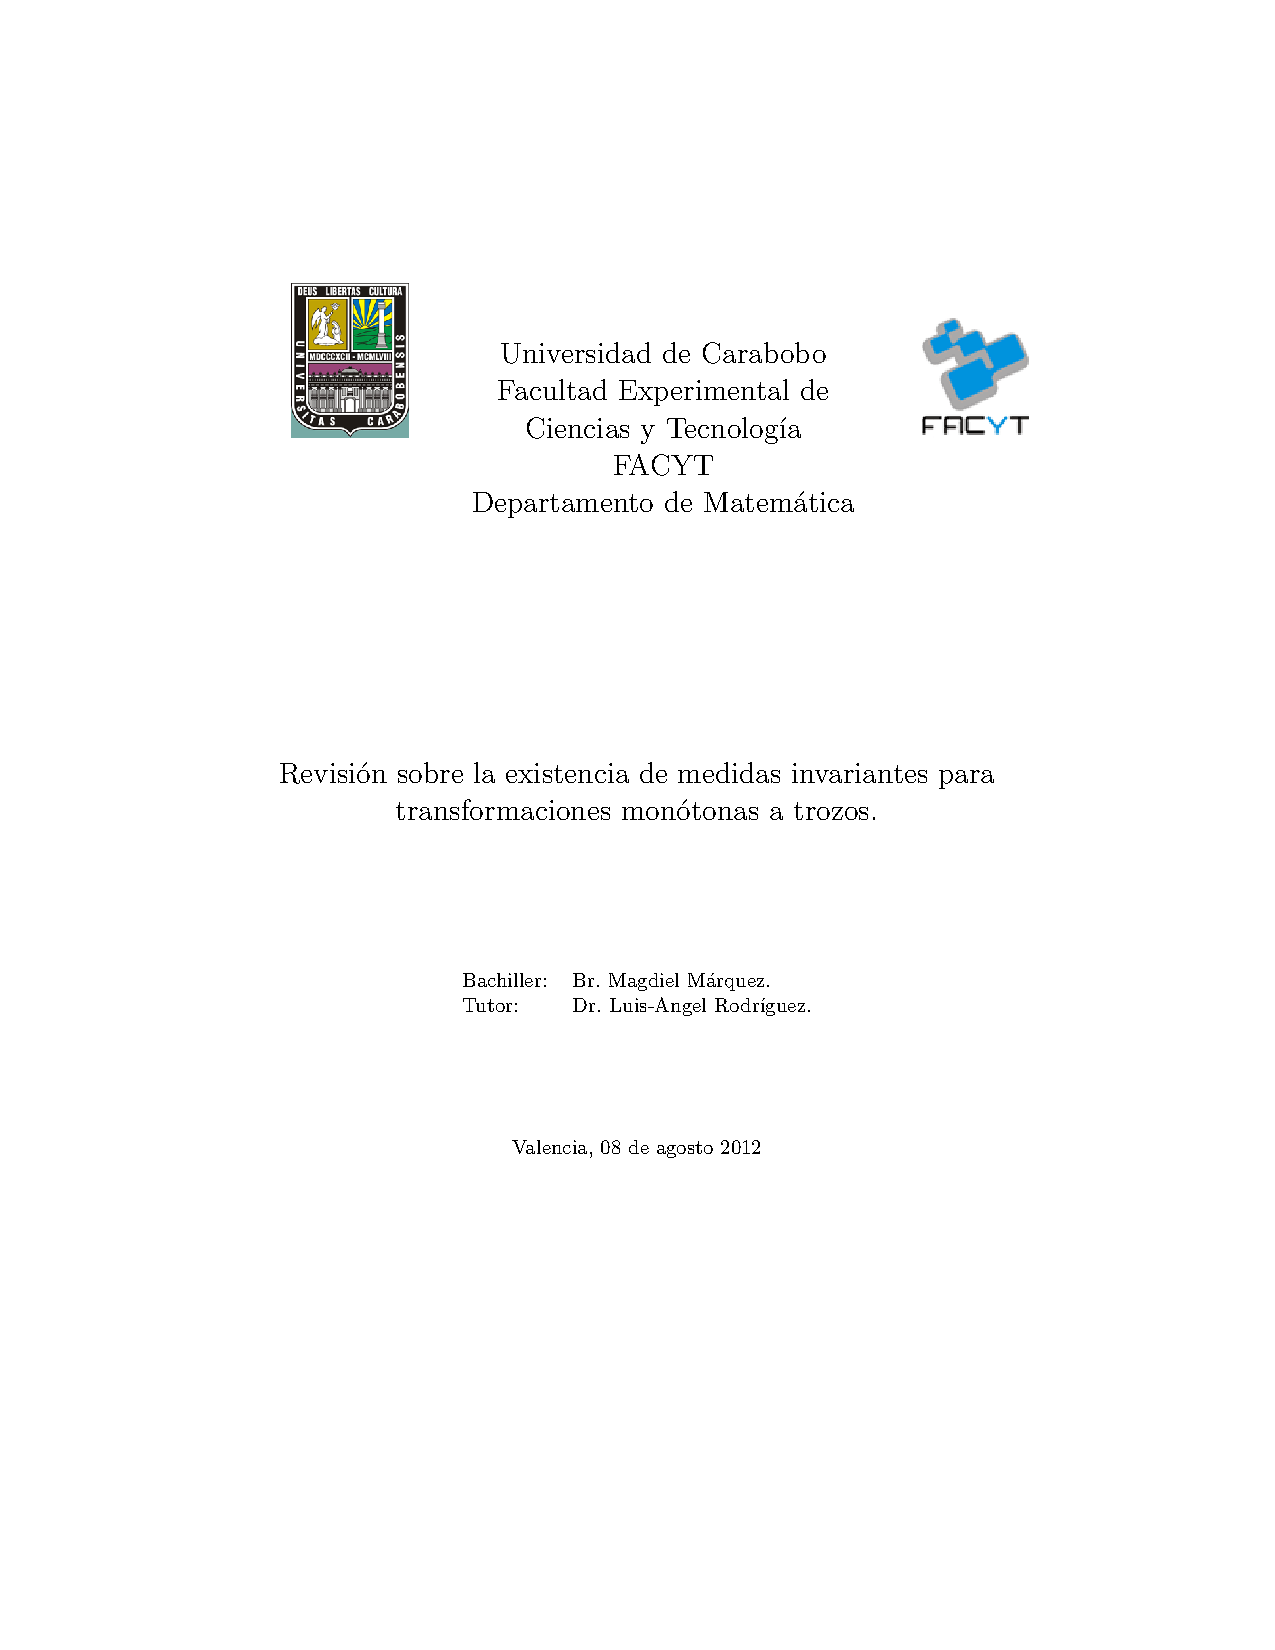
\includegraphics{graficas/tesis.2}\\
    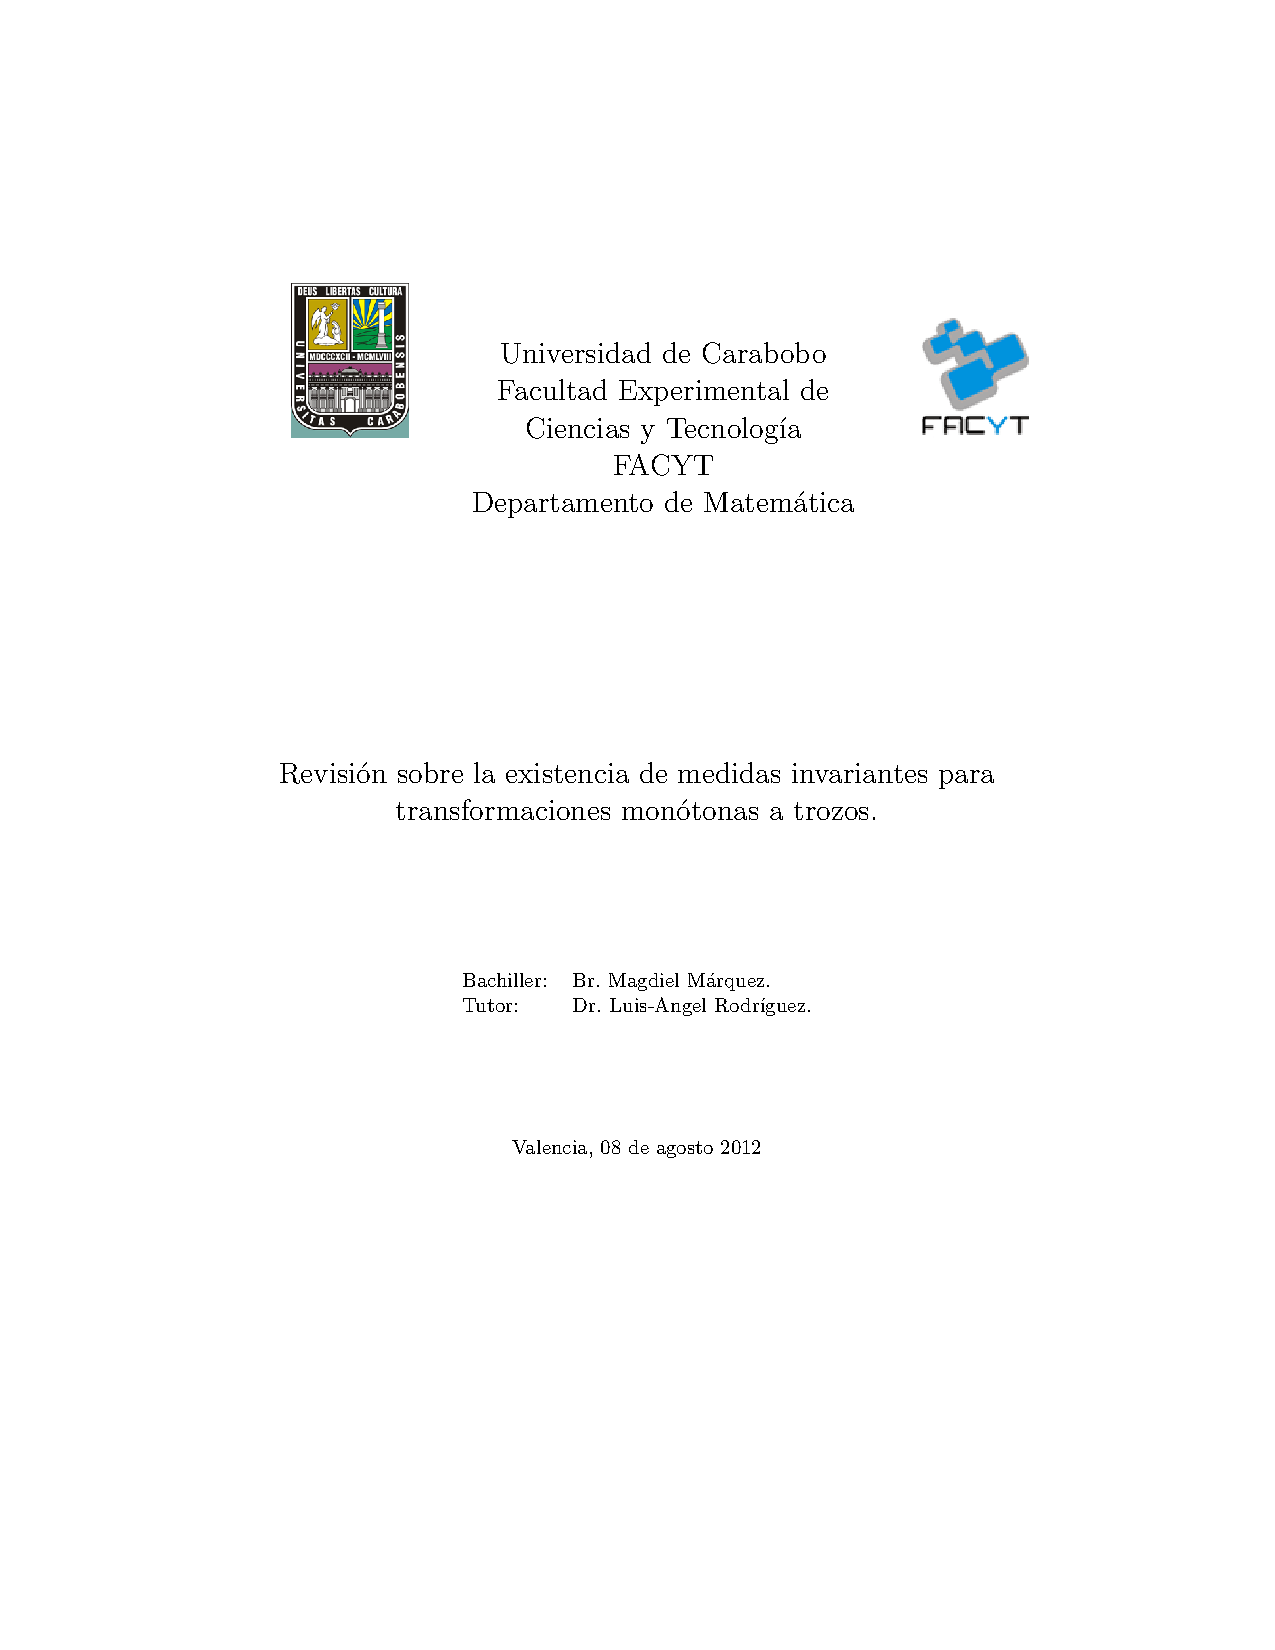
\includegraphics{graficas/tesis.3}
        \begin{picture}(0,0)
        \end{picture}
    \end{center}
    \caption{(Arriba) La trayectoria de $S(x)$ con condici�n inicial $x^0=\pi/10$.
     (Abajo) Trayectoria de $S(x)$ con condici�n inicial $x^1=\pi/10+0.001$ }
     \label{OClogistica}
\end{figure}

Se considera

$$X^0=\{x^0(0), S(x^0)=x^0(1), S(S(x^0))=x^0(2),\ldots,x^0(n) \}$$
$$X^1=\{x^1(0), S(x^1)=x^1(1), S(S(x^1))=x^1(2),\ldots,x^1(n) \}$$

Y calculando la norma 2, osea

\begin{align*}
    ||x^0-x^1||&=\sqrt{\sum^{n}_{i=0}{x^0(i)-x^1(i)}}\\
               &=35,909\\
\end{align*}

La norma $||x^0-x^1||$ es mayor que 1 y dado que la diferencia entre $x^0$ y $x^1$ es de una mil�sima.
Lo anterior, indica que la soluci�n es sensible a las condiciones in�ciales. Se realiza un estudio estad�stico de cada
una de las trayectorias. Consideremos el histograma de frecuencia $f_i$; este se construye de la siguiente forma.
Se toma una partici�n $\{I_k\}_k=1,\ldots,n$ del espacio de fases $[0,1]$ y para cada trayectoria definimos las frecuencias

$$f_i=\frac{\sharp\{ x^0(j)\in I_k\}}{N}$$

donde $\sum{f_i}=1$, $N>>n$ y $[\frac{\imath-1}{n},\frac{\imath}{n})\;
\imath=1,\ldots,n$. Por ultimo, se grafica la partici�n $\{ I_k \}$ vs la frecuencia $f_i$.

\begin{table}[ht!]
    \begin{tabular}{cc}
          \includegraphics[width=55mm]{graficas/Fig4.jpeg}
          &
          \includegraphics[width=55mm]{graficas/Fig5.jpeg}
    \end{tabular}
    \caption{ (Izquierda) Histograma de frecuencia para $S(x^0)$ con $x^0=\pi/2$.(Derecha)
     Histograma de frecuencia para $S(x^0)$ con $x^0=\pi/2+0.001$.}
    \label{histograma}
\end{table}

Se observa simetr�a en el resultado. Las frecuencia son mayores los extremos $0$ y $1$, pero menores pr�ximos al centro en $\frac{1}{2}$.
Repitiendo este proceso para distintos estados in�ciales, o sea, para distintos valores de $x^0$ y $x^1$ se obtiene, en general, el mismo resultado.
\textit{La trayectoria del sistema es sensible a peque�os cambios en el estado inicial, pero estos no producen cambios
considerables en la distribuci�n de estados}

El estudio de orbitas particulares parece poco fruct�fero, no obstante el an�lisis de las densidades se observa m�s prometedor.
Sin embargo, surgen la varias interrogantes: �C�mo podemos calcular la funci�n de densidad? Y m�s importante a�n, �Existe dicha funci�n
de densidad? �Para cuales condiciones?  En la siguiente secci�n se tratara estos temas.

\section{La evoluci�n de las densidades}

Si considerando que las trayectorias son aleatorias, equidistribuidas e independientes;
hip�tesis de la Ley Fuerte de Grandes N�meros nos permite decir que:

$$Lim_{N\rightarrow\infty}{\sum^{N}_{j=1}{\car_{\tri_0}(x^0_j)}}=\int_{\tri_0}{f_0(x)\mu(dx)}$$

donde $f$ es una funci�n de densidad de $\X$ y se define

\begin{dfn}(Funci�n Caracter�sticas, $\car_\tri (x)$)\label{caracte} Se define como:
    \begin{equation}
     \car_\tri (x)=
	   \begin{cases}
		  1 & Si\; x\in\tri\\	
          0 & Si\; x \;not\in\tri
        \end{cases}
    \end{equation}
\end{dfn}

Sin embargo, debido a la forma como son generados las trayectorias estas no son independientes; por lo que se necesita recurrir a
teoremas Erg�dicos. Los teoremas Erg�dicos pueden pensar se como generalizaciones de las Ley fuerte en caso que no se cumpla la hipostesis independencia.
Se presentar� el operador Perron-Frobenius de forma intuitiva, con la finalidad de poder conseguir la funci�n de probabilidad para
el ejemplo en estudio.

Inicialmente, se supone que tenemos la transformaci�n $S:[0,1]\cir$ (una forma abreviada de decir $S[0,1]$
en s� misma). Se recoge un gran n�mero $N$ de estados in�ciales

$$x_1^0, x_2^0, x_3^0,\ldots, x_N^0$$

Para cada uno de los estados se le aplica la transformaci�n  S, obteniendo  as� $N$ nuevos estados denotados por

$$x_1^1=S(x_1^0), x_2^1=S(x_2^0), \ldots, x_N^1=S(x_n^0)$$

En t�rminos generales, decimos que una funci�n $f_0(x)$ es una funci�n de densidad para el valor inicial
$x_1^0, x_2^0, x_3^0,\ldots, x_N^0$ si, para cada intervalo (no tan peque�o) $\tri_0\subset[0,1]$ tenemos

\begin{equation}
    \int_{\tri_0}{f_0(\mu)d\mu}\simeq\frac{1}{N}\sum_{j=1}^{N}{\car_{\tri_0}(x_j^0)}\label{c1n1}
\end{equation}

Similarmente, la funci�n densidad $f_1(x)$ para los estados $x_1^1, x_2^1, x_3^1,\ldots, x_N^1$ la satisface por $\tri\subset[0,1]$

\begin{equation}
    \int_{\tri}{f_1(\mu)d\mu}\simeq\frac{1}{N}\sum_{j=1}^{N}{\car_\tri(x_j^1)}\label{c1n2}
\end{equation}

Se quiere encontrar la relaci�n entre $f_1$ y $f_2$. Para hacer esto es necesario introducir la noci�n de imagen inversa.

\begin{dfn}(Imagen inversa de $S$, $S^{-1}(\tri)$) Es el conjunto de todos los puntos que estan en $\tri$ luego la aplicaci�n de S, o
$$S^{-1}(\tri)=\{x:S(x)\in\tri\}$$
\end{dfn}

Observe que para cualquier $\tri\subset[0,1]$ se tiene

$$x^1_j\in\tri\qquad sii\quad x_1^0\in S^{-1}(\tri)$$

En consecuencia, se deduce la �til relaci�n

\begin{equation}
    \car_\tri(S(x))=\car_{S^{-1}(x)}(x)\label{c1n3}
\end{equation}

Con \ref{c1n3} ee puede reescribir la ecuaci�n como

\begin{equation}
    \int_\tri{f_1(\mu)d\mu}\simeq\frac{1}{N}\sum_{j=1}^N{\car_{S^{-1}(\tri)}(x_j^0)}\label{c1n4}
\end{equation}

Siendo $\tri_0$ y $\tri$ ha sido arbitraria hasta este punto, simplemente, escogemos $\tri_0=S^{-1}(\tri)$. Con esta opci�n la
ecuaciones \eqref{c1n1} y \eqref{c1n4} son iguales y por lo tanto

\begin{equation}
    \int_\tri{f_1(\mu)d\mu}=\int_{S^{-1}(\tri)}{f_0(\mu)d\mu}\label{c1n5}
\end{equation}

Esta ecuaci�n nos entrega la relaci�n que existe entre las funciones densidad $f_0$ y $f_1$ , y nos dice como
cambia la densidad para los estados iniciales al aplicarles la transformacion $S$. Es decir , nos dice como la
funci�n densidad $f_0$ es cambiada a una nueva funci�n $f_1$ al aplicar la transformacion $S$.
Ahora bien: si $\tri$ es un intervalo , digamos $\tri=[a,x]$ , entonces podemos obtener una
representacion explicita para $f_1$ .En este caso, la ecuaci�n \eqref{c1n5} se transforma en :

$$\int_a^x{f_1(\mu)d\mu}=\int_{S^{-1}([a,x])}{f_0(\mu)d\mu}$$

derivando con respecto a $x$ tenemos

\begin{equation}
    f_1(x)=\frac{d}{dx}\int_{S^{-1}([a,x])}{f_0(\mu)d\mu}\label{c1n6}
\end{equation}

Ahora es claro que $f_1$ depender� de $f_0$.Esta dependencia se indica usualmente escribiendo $f_1=\Pm f_0$
y entonces podemos escribir la ecuaci�n  como :

\begin{equation}
    Pf(x)=\frac{d}{dx}\int_{S^{-1}([a,x])}{f(\mu)d\mu}\label{c1n7}
\end{equation}

Este operador \eqref{c1n7} se le conoce como el nombre de Perron-Frobenius. Para ilustrar el uso de esta formula 
\eqref{c1n7} el resultado en el ejemplo ya estudiado.
Se procede a calcular la regi�n de la inversa de S. Esto se puede hacer despejado la funci�n con respecto a y

\begin{align*}
    4x(1-x)&=y         \\
\intertext{Se despeja x. Operando la expresi�n resulta as�}
          x&=\frac{2\mp 2\sqrt{(1-y)}}{4}  \\%\text{elevando al cuadrado}\\
\end{align*}

Se obtiene la region de integraci�n.

$$S^{-1}([0,x])=[0,\frac{1}{2}-\frac{1}{2}\sqrt{1-x}]\cup[\frac{1}{2}+\frac{1}{2}\sqrt{1-x},1]$$

Sustituyendo en  se obtiene

\begin{align}
    \Pm f(x)&=\frac{d}{dx}\int_{[0,\frac{1}{2}-\frac{1}{2}\sqrt{1-x}]\cup[\frac{1}{2}+\frac{1}{2}\sqrt{1-x},1]}{f(u)du} \nonumber\\
            &=\frac{d}{dx}\int^{\frac{1}{2}-\frac{1}{2}\sqrt{1-x}}_0{f(u)du}+\frac{d}{du}\int^1_{\frac{1}{2}+\frac{1}{2}\sqrt{1-x}}{f(u)du}\nonumber\\
%\intertext{Suponiendo que \frac{dF}{dx}=f}
            &=\frac{d}{dx}F\Bigg(\frac{1}{2}-\frac{1}{2}\sqrt{1-x}\Bigg)
            -\frac{d}{dx}F(0)+\frac{d}{dx}F(1)-\frac{d}{dx}F\Bigg(\frac{1}{2}+\frac{1}{2}\sqrt{1-x}\Bigg)\nonumber\\
            &=\frac{1}{4\sqrt{1-x}}\Bigg\{f\Bigg(\frac{1}{2}-\frac{1}{2}\sqrt{1-x}\Bigg)+f\Bigg(\frac{1}{2}+\frac{1}{2}\sqrt{1-x}\Bigg)\Bigg\}\label{c1n8}
\end{align}

Supongamos que $f(x)=1$ para $x\in [0,1]$. Entonces la formula \eqref{c1n8} se simplifica como

\begin{equation}\label{c1n9}
    \Pm f(x)=\frac{1}{2\sqrt{1-x}}
\end{equation}

Ahora se sustituye la expresi�n \eqref{c1n8}, es decir $\Pm f$ por $f$ y podemos calcular nuevamente

\begin{align}\label{c1n10}
    \Pm(\Pm f(x))&=\Pm^2f(x) \nonumber\\
                 &=\frac{1}{4\sqrt{1-x}}\Bigg\{\frac{1}{2\sqrt{1-\frac{1}{2}+\frac{1}{2}\sqrt{1-x}}}+
                 \frac{1}{2\sqrt{1-\frac{1}{2}-\frac{1}{2}\sqrt{1-x}}}\Bigg\}\nonumber\\
                 &=\frac{\sqrt{2}}{8\sqrt{1-x}}\Bigg\{\frac{1}{\sqrt{1+\sqrt{1-x}}}+\frac{1}{\sqrt{1-\sqrt{1-x}}}\Bigg\}
\end{align}

Se puede mostra que para este ejemplo en especifico la sucesi�n de orbitas converge a una densidad limite dada por:

\begin{equation}\label{c1n12}
    f_*(x)=\frac{1}{\pi \sqrt{x(1-x)}}
\end{equation}

\begin{figure}[ht!]
    \begin{center}
        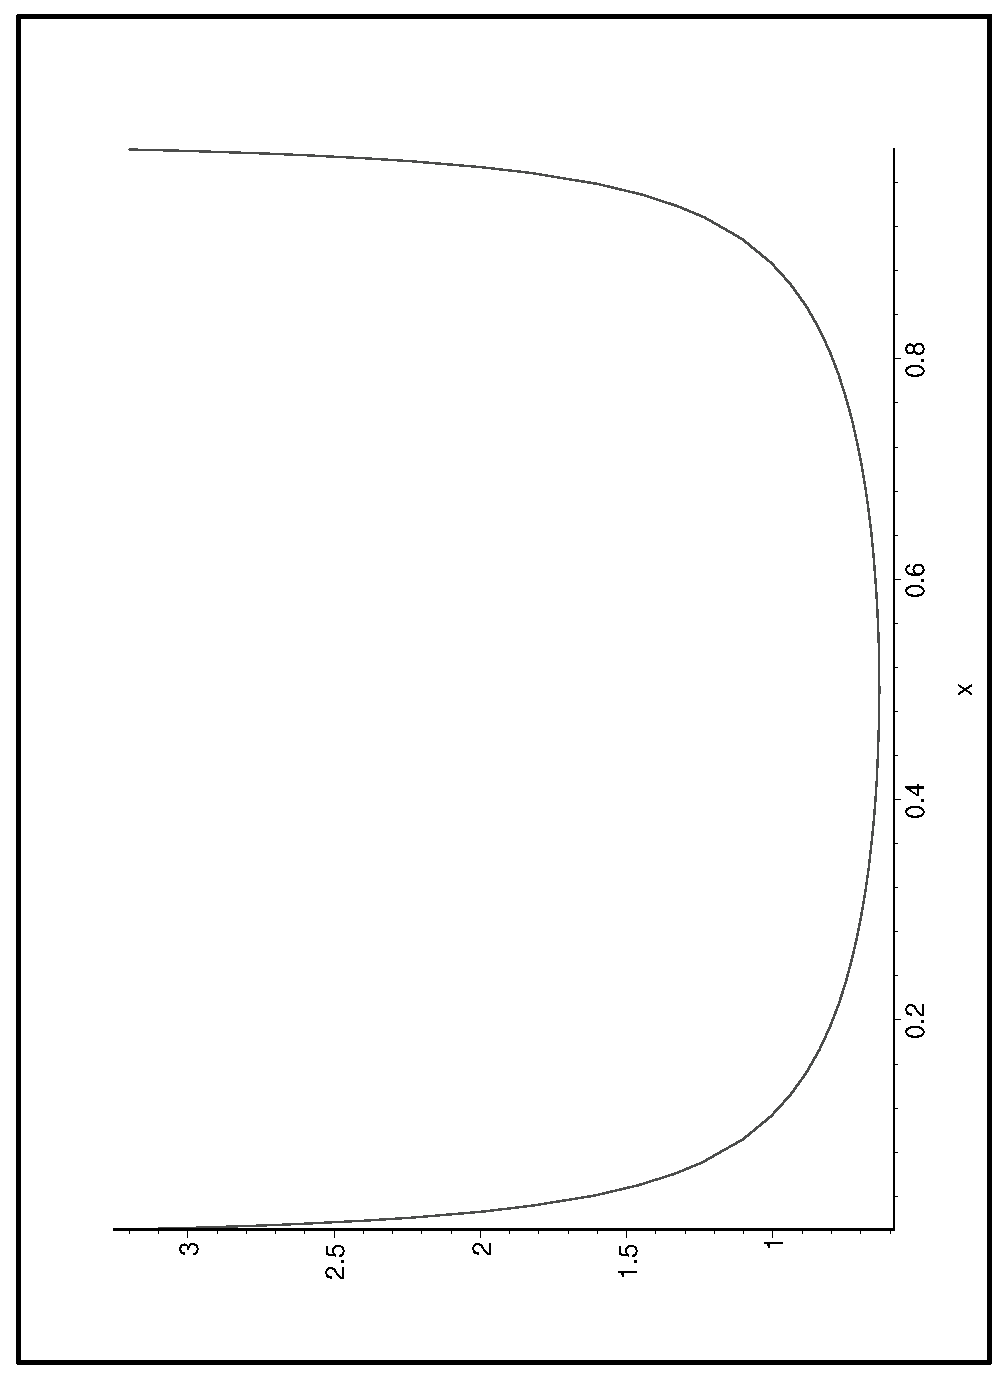
\includegraphics[angle=-90,scale=0.4]{graficas/log2}
    \end{center}
    \caption{Gr�fica $f_*(x)=\frac{1}{\pi \sqrt{x(1-x)}}$. Se observa como la funci�n predice la probabilidad emp�rica consegu�da en los histogramas \ref{histograma}}
    \label{Glimite}
\end{figure}

En la Figura \ref{Glimite} se muestra la gr�fica de la densidad l�mite. Comparando los histogramas \ref{histograma} con \ref{Glimite}
se observa el operador de Perron-Frobenius Refe construye  la  densidad de probabilidad, aunque las condiciones para la
existencia no han sido tratadas. El \emph{estudio de la existencia} ser� el tema a desarrollar en la presente investigaci�n.
As� mismo, como las razones que justifican el paso al l�mite de \eqref{c1n12} y en profundizar en las propiedades del
operador de Perron-Frobenius.

Recapitulando, debido a la sensibilidad a las condiciones in�ciales de algunas funciones se opta en tratar un
problema determinista como un problemaestoc�stico. Enti�ndase como problema determinista hallar el comportamiento
asint�tico de la soluci�n de una ecuaci�n diferencial. As� mismo, como problema estoc�stico el de encontrar  la
funci�n de probabilidad que siguen las trayectorias. Se mostr� como el operador de Perron-Frobenius colabora en
proporcionado un m�todo recursivo para encontrar una sucesi�n que converge a la funci�n de probabilidad deseada. Aunque,
no qued� claro el paso al l�mite de la sucesi�n anterior. Menos aun, las hip�tesis y razonamiento que justifique el 
procedimiento anterior. Estos temas ser�n tratado en del desarrollo de la investigaci�n.



\chapter{Operadores Especiales}

En este cap�tulo se formalizar� y caracterizar �l operador Perron-Frobenius el cual fu� presentado en el Cap�tulo 1.
En dicho cap�tulo se mostr� su uso en estudio de la evoluci�n de densidades bajo la operaci�n de sistemas determin�sticos.

Sin embargo, primeramente se desarrollar�n conceptos generales del operador de Markov. El motivo para este desarrollo preliminar se basa en:
\begin{enumerate}
    \item Muchos conceptos sobre el comportamiento asint�tico de las densidades pueden  ser igualmente formulada por ambos
        sistemas deterministas y  estoc�sticos.
    \item Muchos de los resultados que desarrollamos en los cap�tulos siguientes sobre el  comportamiento de la densidad de la evoluci�n
        bajo la influencia de los  sistemas deterministas, son casos especiales de resultado m�s general para sistemas  estoc�sticos.
\end{enumerate}

Para finalizar, se estudiar� el operador de Koopman el cual est� �ntimamente relacionado con el operador de Perron-Frobenius.

\section{Operador de Markov}

\begin{dfn}[Operador de Markov,$\Pm$] Es un operador lineal $\Pm:L^1\cir$ de un espacio de medida $(\X,\A,\mu)$ que satisface:
    \begin{align*}
            \Pm f&\geq 0     && \text{para  } f\geq 0,\; f\in L^1 \\
            ||\Pm f||&=||f|| && \text{para  } f\geq 0,\; f\in L^1
    \end{align*}
\end{dfn}

\paragraph{Propiedades del Operador de Markov} Si $(\X,\A,\mu)$ es un espacio de medida y $\Pm$ un operador de Markov entonces,
para cada $f,g\in L^1$
    \begin{align}
        \Pm f(x)&\geq \Pm g(x)\phantom{h}  && \hbox{cuando  $f(x)\geq g(x)$}\\
        (\Pm f(x))^+&\leq \Pm f^+(x)       && \\
        (\Pm f(x))^-&\leq \Pm f^-(x)       && \\
        |\Pm f(x)|&\leq \Pm |f(x)|         && \\
        ||\Pm f||&\leq ||f|| \phantom{hool}&&
    \end{align}

\begin{proof} Las demostraciones se deducen directamente de las definciones.
    \begin{align*}
            f\geq g &\Rightarrow f-g\geq 0       &&   \hbox{(despejando)}               \\
                    &\Rightarrow h\geq 0         &&   (h=f-g \in L^1)                   \\
                    &\Rightarrow \Pm h\geq 0     &&   \hbox{(def. operador de Markov)}  \\
                    &\Rightarrow \Pm(f-g)\geq 0  &&   \hbox{(sustituyendo h)}           \\
                    &\Rightarrow \Pm f\geq \Pm g &&   \hbox{(por linealidad)}
    \end{align*}

    Cuando un operador satisface se dice que es montomo.

    \begin{align*}
            (\Pm f(x))^+  &= (\Pm (f^+(x)-f^-(x)))^+          && \hbox{(por col. de $f$)}                \\
                          &= (\Pm f^+(x)-Pf^-(x))^+           && \hbox{(por linealidad)}                 \\
                          &= \max{\{0,\Pm f^+(x)-\Pm f^-(x)\}}&& \hbox{(def. de $f$ positiva)}           \\
                          &= \max{\{0,\Pm f^+(x)\}}           && \hbox{(debido a $Pf^-(x)\geq 0$)}    \\
                          &= \Pm f^+(x)                       && \hbox{(def. de $f$ positiva )}
    \end{align*}

    Con lo que se demuestra . La propiedad  es similar.

    \begin{align*}
            (\Pm f(x))^-  &=    (\Pm (f^+(x)-f^-(x)))^-          && \hbox{(por col. de $f$)}                  \\
                          &=    (\Pm f^+(x)-Pf^-(x))^-           &&\hbox{(por linealida)}                     \\
                          &=    \max{\{0,\Pm f^-(x)-\Pm f^+(x)\}}&&\hbox{(def. de $f$ negativa)}              \\
                          &\leq \max{\{0,\Pm f^-(x)\}}           &&\hbox{(debido a $Pf^-(x)\geq 0$)}          \\
                          &=    \Pm f^-(x)                       &&\hbox{(def. de $f$ negativa)}
    \end{align*}

    En la propiedad se incluyen los resultados presendentes.

    \begin{align*}
            |\Pm f(x)| &=   (\Pm f(x))^+ +(\Pm f(x))^- && \hbox{(por col. de $f$)}                         \\
                       &\leq \Pm f^+(x)+\Pm f^-(x)     && \hbox{(por  y )}   \\
                       &=    \Pm (f^+(x)+f^-(x))       && \hbox{(por linealidad)}                          \\
                       &=    \Pm |f(x)|                && \hbox{(por col. de $f$)}
    \end{align*}

   Y la propiedad de mayor importancia

    \begin{align*}
            ||\Pm f(x)|| &=    \int_\X |\Pm f(x)|\mu(dx) && \hbox{(por definici�n de norma)}               \\
                         &\leq \int_\X \Pm |f(x)|\mu(dx) && \hbox{(por )}                   \\
                         &=    \int_\X |f(x)|\mu(dx)      && \hbox{(def. Operador de Markov )} \\
                         &=    ||f(x)||                 && \hbox{(por def. de norma)}
    \end{align*}
\end{proof}

Se ilustra la importancia de la propiedad . Note que para cualquier operador $f \in L^1$ se tiene

\begin{align}
    ||\Pm^{n+1}f||&=||\Pm(\Pm^{n}f)|| && \hbox{debido a } \Pm:\cir\nonumber\\
                  &\leq||\Pm^{n}f||   &&\hbox{por }
\end{align}

Graficando la inecuaci�n

\begin{figure}[ht!]
    \begin{center}
        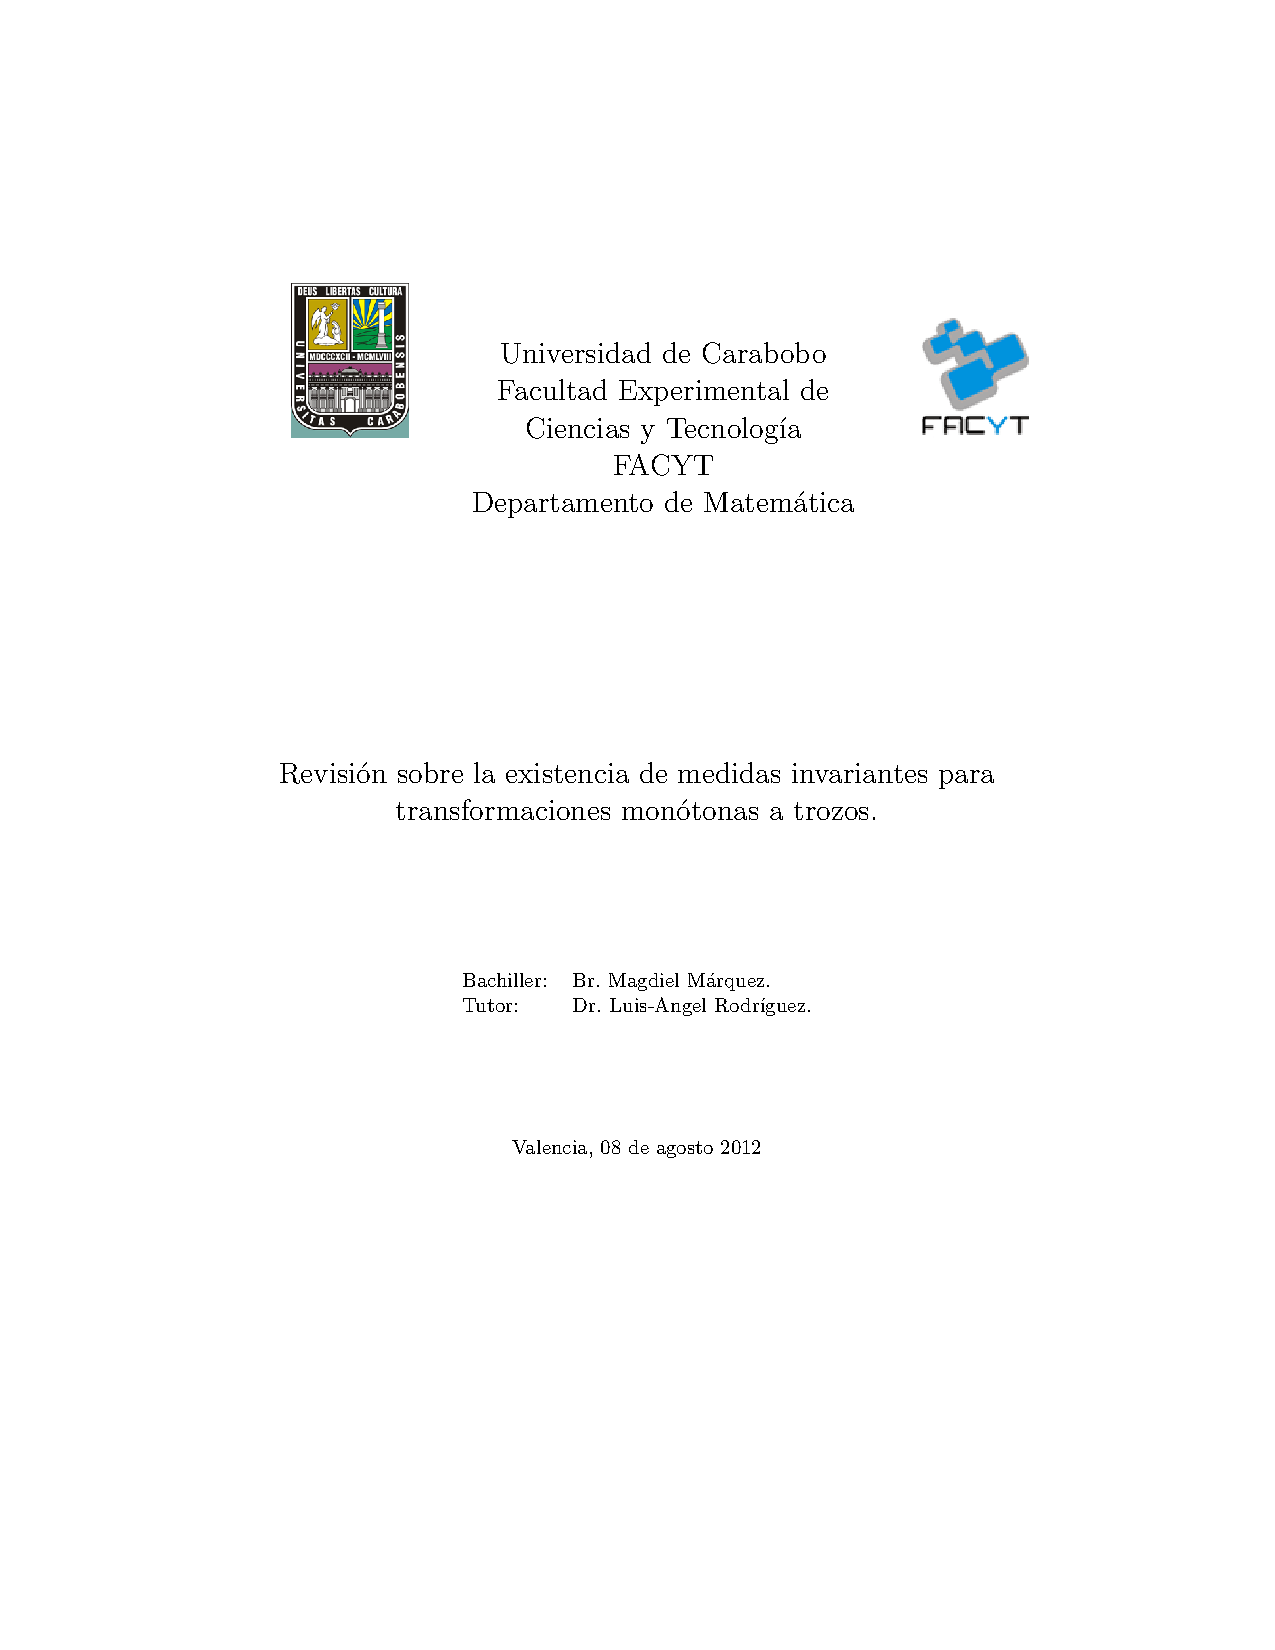
\includegraphics{graficas/tesis.7}
        \put(-90,80){$\Pm^{n+2} f$}
        \put(-70,97){$\Pm^{n+1} f$}
        \put(-50,112){$\Pm^{n}  f$}
   \end{center}
   \caption{Con cada iteraci�n del operador la �rbita el operador decrece o se mantiene.}
\end{figure}


A esta propiedad se le conoce con el nombre de contractiva debido a que reduce la distancia en el proceso de iteraci�n.
Como se puede observar para cualquier par de funciones distintas de $L^1$.


\begin{align}
||\Pm^{n+1}f_1-\Pm^{n+1}f_2||&=||\Pm^{n+1}(f_1-f_2)||   && \text{linealidad}  \nonumber         \\
                     &\leq||\Pm^{n}(f_1-f_2)||          && \text{por } \nonumber    \\
                     &=||\Pm^{n}f_1-\Pm^{n}f_2||        &&
\end{align}

Graficando la inecuaci�n

\begin{figure}[ht!]
    \begin{center}
        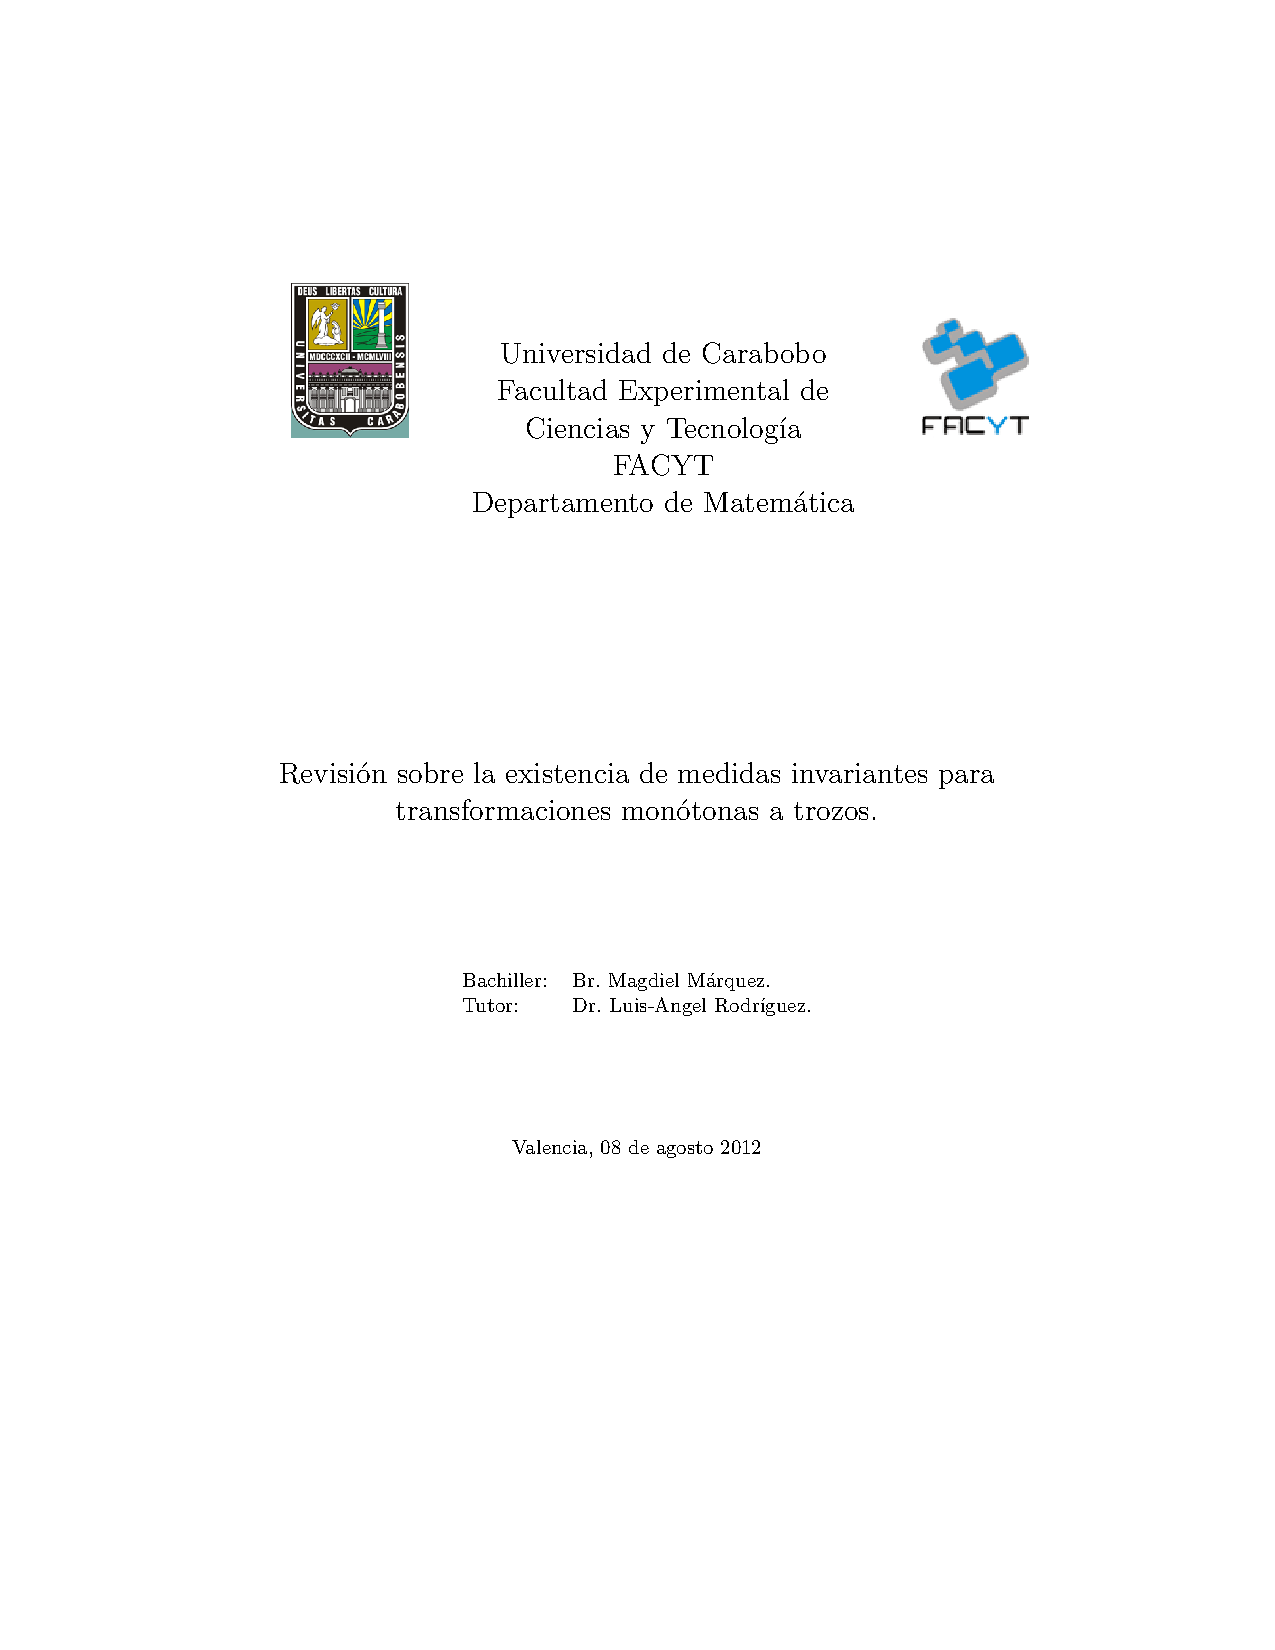
\includegraphics{graficas/tesis.8}
        \put(-255,40){$\Pm^{n}f_1$}
        \put(-265,25){$\Pm^{n+1}f_1$}
        \put(-265,10){$\Pm^{n+2}f_1$}
        \put(-255,-5){$\Pm^{m}f_2$}
   \end{center}
   \caption{Sea $\Pm^i f_2=\Pm^m f_2  \quad \forall i\in\N$, �sea un punto fijo. Se aprecia como la norma $ ||\Pm^{i} f_1-\Pm^{i} f_2||$ se reduce con cada iteraci�n, acerc�ndose  $\Pm^{i} f_1$ de $\Pm^{i} f_2$.}
\end{figure}

De lo analizado se desprende la idea de orbitas acotadas o orbitas estables. Se formalizar� esta noci�n con la siguiente definici�n.

\begin{dfn}[Estabilidad de la iteraciones] Es cuando la distancia entre un par de funciones, durante el proceso de iteraciones, puede decrecer
 pero jam�s aumentar.
\end{dfn}

\begin{dfn}[Soporte de una funci�n g(x),$\so g(x)$] Son todos los x del dominio donde g(x) no se anula.
\end{dfn}

\subparagraph{Observaci�n} Esta no es la definici�n usual de soporte de una funci�n, normalmente se define como
$$\so g=clausura\{x:g(x)\neq 0 \}$$
No obstante, debido a que requiere conceptos topol�gicos se prefiri� usar esta definici�n no tan com�n.


\begin{pro} Sea $||\Pm f||=|| f||$ sii $\Pm f^+$ y $\Pm f^-$ son soportes disjuntos
\end{pro}\label{teopro}

\begin{proof} Notemos que si $x\geq0$ e $y\geq0$
\begin{align*}
    -x&\leq x & -y&\leq y                                              \\
    -y-x&\leq x-y & x-y&\leq x+y                                         \\
    -(x+y)&\leq x-y \leq x+y &  &  \\
    |x-y|&\leq x+y   & &\\
    |x-y|&\leq|x+y|   &\hbox{Ya que $x>0\; \& \; y>0$} &                \\
\end{align*}


Por lo tanto podemos afirmar
\begin{align*}
    |\Pm f^+-\Pm f^-|&\leq|\Pm f^++\Pm f^-|                                 \\
                     &\leq|\Pm f^-|+|\Pm f^-|   && \hbox{desigualdad triangular}
\end{align*}
    La desigualdad estricta se cumple para cualquier $\Pm f^+>0$ y $\Pm f^->0$. La igualdad solo se garantiza cuando $\Pm f^+=0$ o $\Pm f^-=0$.
     Supongase la igualdad (Osea $\Pm f^+=0$ o $\Pm f^-=0$) e integrando sobre el espacio tenemos
\begin{equation}
    \int_\X|\Pm f^+-\Pm f^-|\mu(dx)=\int_\X|\Pm f^+|+\int_\X|\Pm f^-|\mu(dx)
\end{equation}
por lo tanto se tiene que
\begin{align*}
    \nexists A\subset,&\; \mu(A)>0 \quad \hbox{tal que} \quad  \Pm f^+>0 \quad y\quad \Pm f^->0  \\
\intertext{Como $\Pm f\geq0$, tenemos de la definici�n de soporte vista en OJO}
    \nexists A\subset,&\; \mu(A)>0 \quad \hbox{tal que} \quad A\subset\so(\Pm f^+) \quad y\quad A\subset\so(\Pm f^-)  \\
    \nexists A\subset,&\: \mu(A)>0 \quad \hbox{tal que} \quad A\subset\so(\Pm f^+)\cap\so(\Pm f^-)
\end{align*}
por lo tanto la ecuaci�n en el lado izquierdo quedaria
\begin{align*}
    \int_\X|\Pm f^+-\Pm f^-|\mu(dx)&=\int_\X|\Pm (f^+- f^-)|\mu(dx) && \hbox{Agrupando}       \\
                                   &=\int_\X|\Pm f|\mu(dx)          && \hbox{por col. de $f$} \\
                                   &=||\Pm f||                      &&\hbox{por def. norma}
\end{align*}
mientras que por el lado derecho de
\begin{align*}
\int_\X|\Pm f^+|+\int_\X|\Pm f^-|\mu(dx)&=||\Pm f^+||+||\Pm f^-|| &&\hbox{por def. norma}      \\
                                        &=||f^+||+||f^-||         &&\hbox{por def. de Markov}  \\
                                        &=|(||f ||)|              &&\hbox{por col. de $f$}     \\
                                        &=||f||                   &&\hbox{la norma es positiva}
\end{align*}
por �ltimo agrupando ambos lados de nos queda
$$||\Pm f||=||f|| $$
\end{proof}

La definici�n de punto fijo  se considera en este contexto siendo $\Pm:L^1\cir$ la ley de evoluci�n temporal.
 Se presenta una caracterizaci�n para los puntos fijos del operador de Markov

\begin{pro} Si $\Pm f=f$ entonces $\Pm f^+=f^+$ y $\Pm f^-=f^-$
\end{pro}

\begin{proof} Como $\Pm f=f$ entonces
\begin{align*}
f^+&=(\Pm f)^+\leq \Pm f^+                                                 \\
f^-&=(\Pm f)^-\leq \Pm f^-                                                 \\
\intertext{por lo tanto}
   &(\Pm f)^+ - f^+\geq0                                                   \\
   &(\Pm f)^- - f^-\geq0                                                   \\
\intertext{sumando e integrando las desigualdades}
   &\int_\X{[\Pm f^+ - f^+]\mu(dx)}+\int_\X{[\Pm f^- - f^-]\mu(dx)} \geq  0   \\
   &\int_\X{[\Pm f^+ + \Pm f^-]\mu(dx)}-\int_\X{[ f^+ + f^-]\mu(dx)}  \geq  0 \\
   &\int_\X{\Pm |f|\mu(dx)}-\int_\X{|f|\mu(dx)} \geq    0                     \\
   &||\Pm\; |f|\;|| -||f|| \geq  0                                          \\
\intertext{por otro lado. Gracias a la propiedad contractiva tenemos $||\Pm\; |f|\;|| -||f|| \leq  0 $
en consecuencia se llega a una contradicci�n. Por lo tanto $||\Pm\; |f|\;|| -||f||=0$}
\Pm f^+ - f^+&=0    &  \Pm f^- - f^-&=0 \\
\Pm f^+      &=f^+  &   \Pm f^-     &=  f^-
\end{align*}
\end{proof}

\begin{dfn}[Conjunto de densidades, $D(\X,\A,\mu)$] Es el conjunto
definido como $\{f\in L^1(\X,\A,\mu):f\geq 0\; \& \; ||f||=1\}$ donde $(\X,\A,\mu)$ es un espacio de medida.
Cualquier funci�n $f\in D(\X,\A,\mu)$ es llamada \textbf{densidad}.
\end{dfn}

\begin{dfn}[Densidad $f$ de $\mu$, $\mu_f(A)$] Si se cumple que
$$\mu_f(A)=\int_A{f(x)\mu(dx)}\qquad \text{para } A\in\A$$
Donde $f\in D(\X,\A,\mu)$. Tambi�n se dice que $f$ es \textbf{absolutamente continua} con respecto a $\mu$.
\end{dfn}

Usando la noci�n de densidades se puede extender el concepto de punto fijo a un operador de Markov con la siguiente definici�n.

\begin{dfn}[Densidad estacionaria] Para cualquier $f\in D$ que satisfaga $\Pm f=f$ siendo $(\X,\A,\mu)$ un espacio de medida y $\Pm$
 un operador de Markov.
\end{dfn}

\subparagraph{Observaci�n} El concepto de densidad estacionaria de un operador jugara un papel fundamenta el los pr�ximos cap�tulos.

\section{El operador Perron-Frobenius}

En el cap�tulo 1 se presento el operador de Perron-Frobenius para el estudiar la evoluci�n de la densidad en el caso de la funci�n log�stica.
  Despu�s de haber desarrollado el concepto de operador de Markov y algunas de sus propiedades; se est� en posici�n de estudiar el operador
  de Perron-Frobenius. En consecuencia, se fundamentar�, se caracterizar� e ilustrar� dicho operador; as� como se mostrar� su relaci�n con
  el operador de Markov.

\begin{lem}Sea $S:\cir$ una transformaci�n no-singular sobre un espacio de medida dado. Sea $f\in L^1$ con $f\geq 0$ la siguiente expresi�n:
    \begin{equation}
        \int_{S^{-1}(A)}{f(x)\mu(dx)}
    \end{equation}
    es una medida y existe un unico elemento en $L^1$, que denotaremos por $\Pm f$, tal que:
    $$\int_A{\Pm f(x)\mu(dx)}=\int_{S^{-1}(A)}{f(x)\mu(dx)} \qquad para \; A\in\A$$
\end{lem}

\begin{proof} Se procede a demostrar que %~\ref{lemPer}
    es una medida. Observe que la imagen inversa del conjunto vacio es vacio por lo tanto
    \begin{align*}
        \int_{S^{-1}(\emptyset)}{f(x)\mu (dx)}&=\int_{\emptyset}{f(x)\mu (dx)} && \\
                                              &=0
    \end{align*}
    Como S es no singular entonces $\mu(S^{-1}(A))\geq 0$ para $\mu(A)\geq 0$
    Por lo tanto podemos garantizar que
    $$\int_{S^{-1}(A)}{f(x)\mu(dx)}\geq 0 \qquad \int_{A}{f(x)\mu(dx)\geq 0}$$
    \begin{align*}
        \intertext{Por ultimo consideremos}
            S^{-1}(\cup_i{A_i}) & =\cup_i S^{-1}{(A_i)}\\
        \intertext{Siendo lo $A_i$ disjuntos se tiene}
            \int_{S^{-1}(\cup_i{A_i})}{f(x)\mu(dx)} & ={\int_{\cup_i S^{-1}{(A_i)}}{f(x)\mu(dx)}}\\
        \intertext{y por la propiedad L5}
            \int_{S^{-1}(A)}{f(x)\mu(dx)} & =\sum_i{\int_{S^{-1}{(A_i)}}{f(x)\mu(dx)}}\\
        \intertext{con los cual es una medida. Como $f\in L^1$ entonces tiene medida finita.}
    \end{align*}
    por lo tanto por el colorario X, existe un unico elemento $f\in L^1$ tal que
    $$\nu(A)=\int_A{f(x)\mu(dx)} \qquad \text{para cada } a\in\A$$
\end{proof}

\begin{equation}
    \int_{A}{\Pm f(x)\mu(dx)}=\int_{S^{-1}(A)}{f(x)\mu(dx)} \qquad para\; A\in\A\label{c2n00}
\end{equation}

\paragraph{Propiedades del Operador Perron-Frobenius} A partir de puede deducir las siguientes propiedades.
    \begin{align}
        \Pm(\lambda_1f_1+\lambda_2f_2)&= \lambda_1\Pm f_1+\lambda_2\Pm f_2 && f_i\in L^1\;y\;\lambda_i\in\R\;(i=1,2)\\
        \Pm\geq 0 \quad &\hbox{si} \quad f\geq 0\\
        \int_{\X}{\Pm f(x)\mu(dx)}&=\int_{\X}{f(x)\mu(dx)}
    \end{align}
    Si $S_n=S\circ\ldots^n\circ S$ y $\Pm_n$ es el operador de Forbenius-Perron correspondiente a $S_n$,
    entonces $\Pm_n=\Pm^n$, donde $\Pm$ es el operador de Forbenius-Perron correspondiente para $S$.
    Las demostraciones son directas de la definici�n en el caso de tenemos

    \begin{align*}
        \Pm(\lambda_1f_1+\lambda_2f_2) &= \int_{A}{\Pm (\lambda_1f_1+\lambda_2f_2)\mu(dx)} \\
        \intertext{Consideremos $B=S^{-1}(A)$}
                                       &= \int_{B}{(\lambda_1f_1+\lambda_2f_2)\mu(dx)}\\%&(\hbox{def. del Operador})\\
                                       &=\lambda_1\int_{B}{f_1\mu(dx)}+\lambda_2\int_{B}{f_2\mu(dx)}\\%&(\hbox{linealidad de la Integral})\\
                                       &= \lambda_1\int_{A}{\Pm f_1\mu(dx)}+\lambda_2\int_{A}{\Pm f_2\mu(dx)}\\% &(\hbox{def. del Operador})
    \end{align*}

La demostraci�n que es una medida nos garantiza que se cumple ya que la medida es una funci�n positiva. Por �ltimo observemos que $S:\X\rightarrow\X$ por lo tanto la imagen inversa de $\X$ esta contenida en $\X$.

\subparagraph{Observaci�n} Las propiedades nos garantizan que el operador de Perron-Frobenius es un operador de Markov y por lo tanto cumple con las propiedades vistas anteriormente.

Para algunos casos especiales se tiene una forma expl�cita del operador de Perron-Frobenius.
Si $\X=[a,b]$ es un intevalo real y $A=[a,x]$ entonces se escribe como

\begin{equation*}
    \int^x_a{\Pm f(s)ds}=\int_{S^{-1}([a,x])}{f(s)ds}
\end{equation*}

derivando respecto a x

\begin{equation}
    \Pm f(x)=\frac{d}{dx}\int_{S^{-1}([a,x])}{f(s)ds}\label{c2n0}
\end{equation}

es importante notar que este es un caso especial donde la transformaci�n $S$ es diferenciable e invertible,
en el cual la forma expl�cita de $\Pm f$ es posible. Si $S$ es diferenciable y invertible entonces es mon�toma,
adicionalmente, supongamos que es creciente y $S^{-1}$ tiene derivada continua. Entonces

\begin{equation*}
    S^{-1}([a,x])=[S^{-1}(a),S^{-1}(x)]
\end{equation*}

por lo tanto queda:

\begin{align*}
    \Pm f(x)&=\frac{d}{dx}\int_{S^{-1}(a)}^{S^{-1}(x)}{f(s)ds}    \\
            &=f(S^{-1}(x))\frac{d}{dx}(S^{-1}(x))
\end{align*}

y si $S(X)$ es decreciente

\begin{align*}
    \Pm f(x)&=\frac{d}{dx}\int_{S^{-1}(x)}^{S^{-1}(a)}{f(s)ds}    \\
            &=\frac{d}{dx}-\int_{S^{-1}(a)}^{S^{-1}(x)}{f(s)ds}   \\
            &=-f(S^{-1}(x))\frac{d}{dx}(S^{-1}(x))
\end{align*}

\begin{pro} Sea $S\circ$ una una transformaci�n real diferenciable e invertible, con derivada continua y creciente
    entonces el operador de Perron-Frobenius se expresa como:
    \begin{equation}
         \Pm f(x)=f(S^{-1})|\frac{d}{dx}[S^{-1}(x)]|\label{c2n1}
    \end{equation}
\end{pro}

\begin{ejm} Veamos como el operador de Perron-Frobenius trabaja. Sea $S(x)=\exp(x)$,
    siendo $S^{-1}=\ln(x)$ y $(S^{-1})'=\frac{1}{x}$. Aplicando \eqref{c2n1} la propiedad tenemos
    $$\Pm f(x)=f(\ln(x))(\frac{1}{x})$$
    Consideremos que ocurre si se toma la densidad de probabilidad $f$ dada por
    $$f(x)=\frac{1}{2}\car_{[-1,1]}(x)$$
    Evaluando la densidad sobre $\Pm$ tenemos
    \begin{figure}
        \begin{center}
            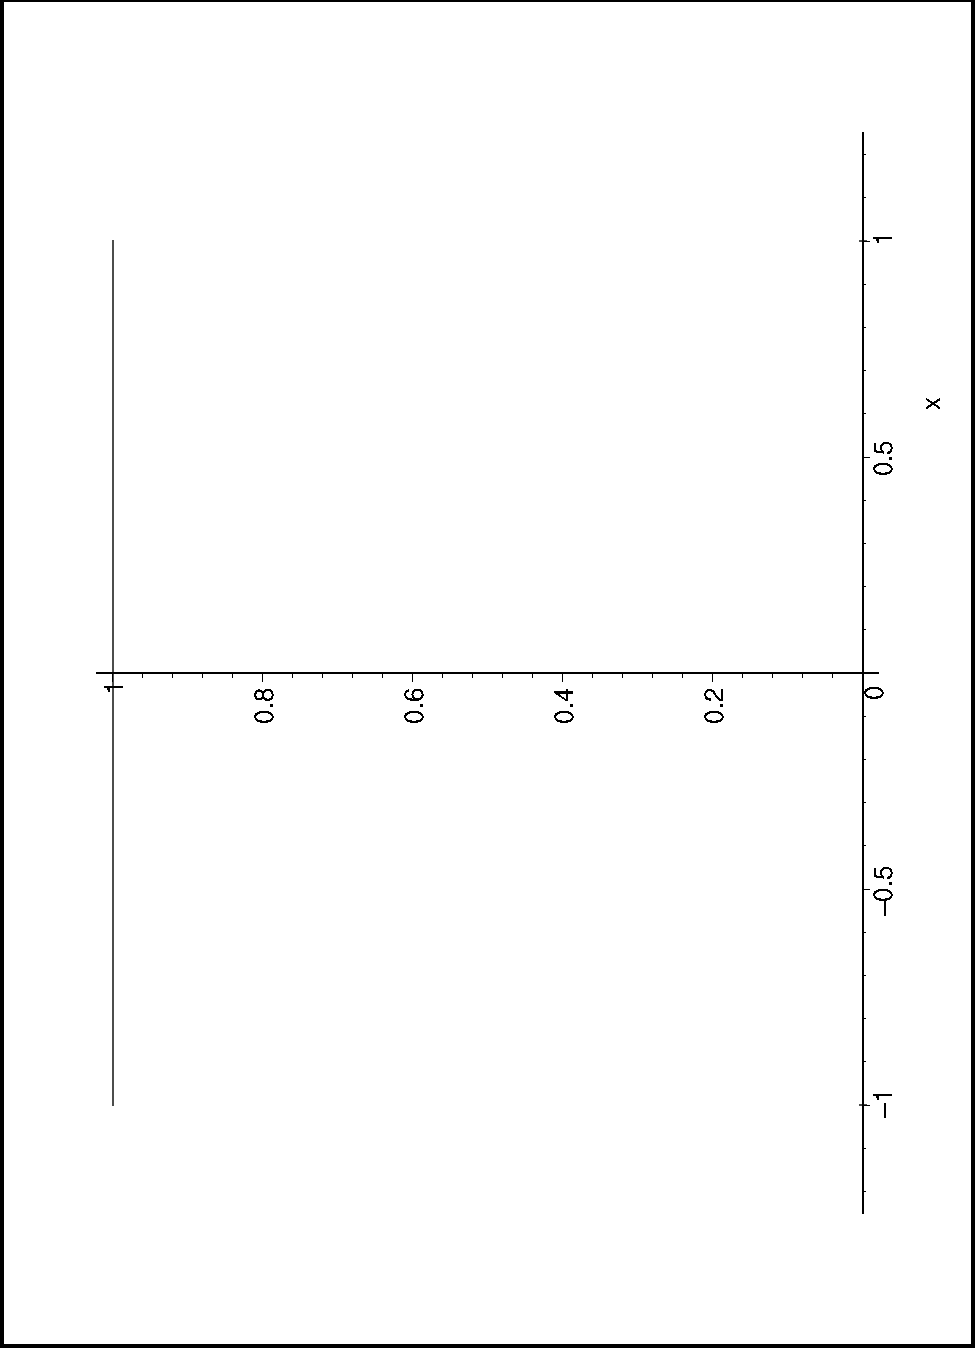
\includegraphics[angle=-90,scale=0.25]{graficas/car}
        \end{center}
        \caption{La gr�fica de $f(x)=\frac{1}{2}\car_{[-1,1](x)}$. Observe que $\int_{-1}^1{f(x)dx=1}$ y por lo tanto $f(x)$ una densidad.}
    \end{figure}

    \begin{align*}
        \frac{1}{2}\car_{[-1,1]}(\ln(x))&=\begin{cases}
                                    \frac{1}{2}& \text{si $-1\leq\ln(x)\leq 1$}\\
                                    0 & \text{en otro caso}
                                \end{cases} \\
                              &=\begin{cases}
                                    \frac{1}{2}& \text{si $e^{-1}\leq x\leq e^{1}$}\\
                                    0 & \text{en otro caso}
                                \end{cases} \\
                              &= \frac{1}{2}\car_{[e^{-1},e^1]}(x)
    \end{align*}
    \begin{figure}
        \begin{center}
            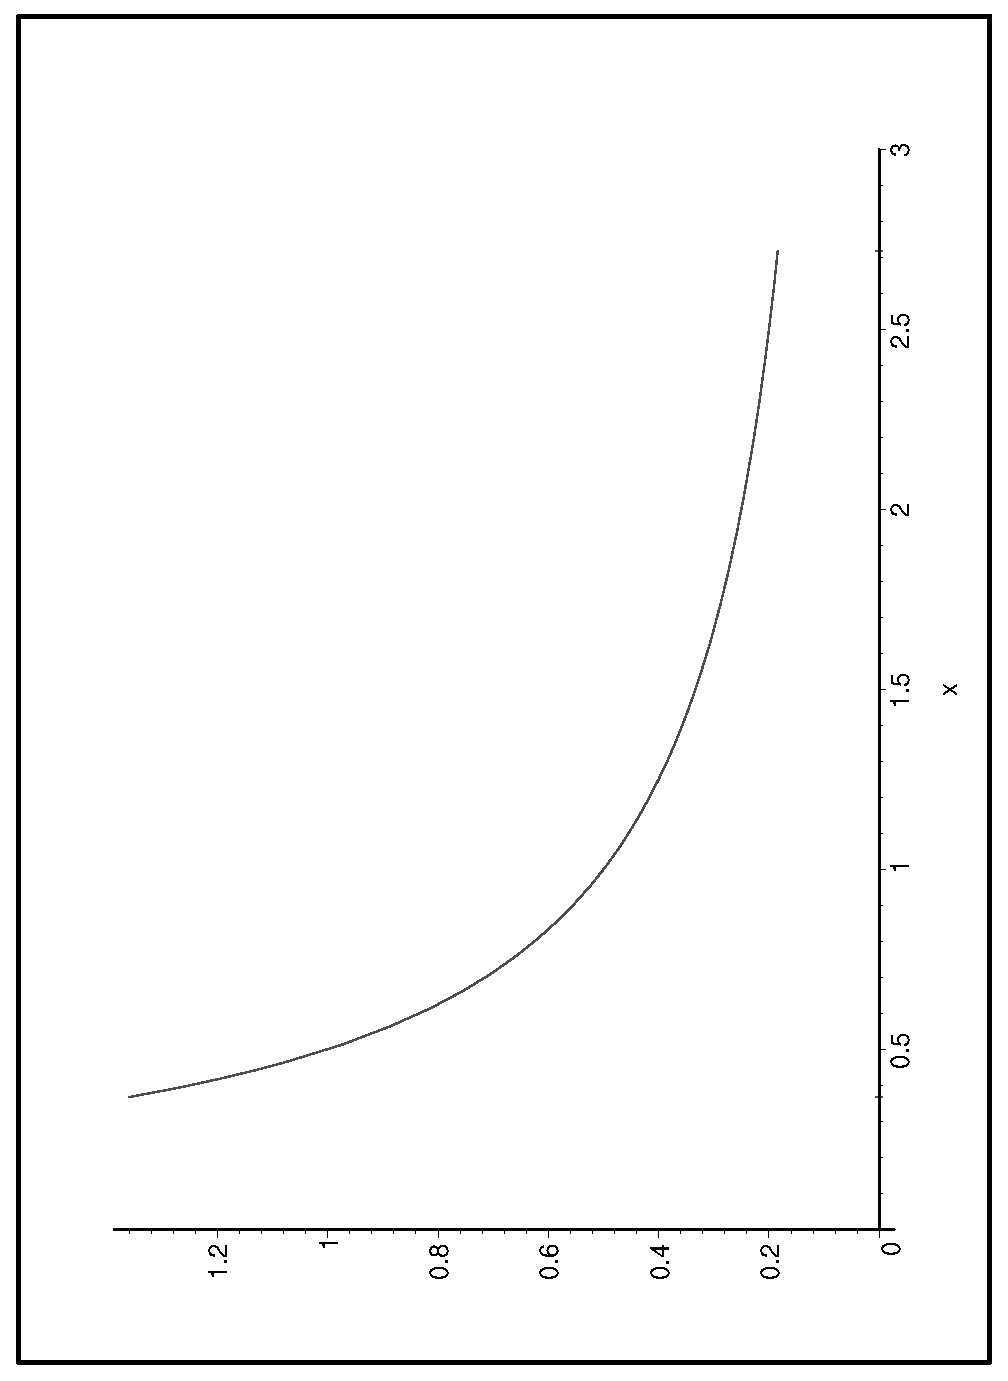
\includegraphics[angle=-90,scale=0.25]{graficas/exp}
        \end{center}
        \caption{La gr�fica de $\Pm f(x)=\frac{1}{2}\car_{[e^{-1},e^1](x)}$.
        Debido a $\int_{-1}^1{f(x)dx=1}$ y por lo tanto $\Pm f(x)$ una densidad. En otra palabra, el operador
        $\Pm$ mapeo una densidad en otra densidad.}
    \end{figure}
\end{ejm}

N�tese que el soporte de la funci�n $f$ est� contenido en el soporte de $\Pm f$. Esa observaci�n la generaliza la siguiente proposici�n

\begin{teo} Sea $S:\X\rightarrow\X$ una transformaci�n no singular y $\Pm$ el operador de Perron-Frobenius.
    Se asume $f\leq 0, f\in L^1$ es dado. Entonces
    \begin{equation}
    \so f\subset S^{-1}(\so \Pm f)\label{c2n2}
    \end{equation}
    Y, m�s generalmente, para cada conjunto $A\in\A$ la siguiente equivalencia es cierta:
    $\Pm f(x)=0$ para $x\in\A$ si y solo si $f(x)=0$ para $x\in S^{-1}(A)$.
\end{teo}

\begin{proof} Por la definici�n del operador de Perron-Frobenius, se tiene
    \begin{align*}
            \int_A\Pm f(x)\mu(dx)&=\int_{S^{-1}(A)}{f(x)\mu(dx)}\\
        \intertext{Que es equivalente a}
            \int_\X{1_A(x)\Pm f(x)\mu(dx)}&=\int_\X{1_{S^{-1}(A)}f(x)\mu(dx)}
    \end{align*}
    As� $\Pm f(x)=0$ sobre $A$ implica, por la propiedad ~\ref{L2} de la integral de Lebesgue, que $f(x)=0$ para
    $x\in S^{-1}(A)$  y viceversa. Se toma $A=\X\backslash\so(\Pm f)$ y se tiene $\Pm f(x)=0$ para $x\in A$ y, en consecuencia,
    $f(x)=0$ para $x\in S^{-1}(A)$ esto significa que $\so f\subset\X\backslash S^{-1}(A)$. Como $S^{-1}(A)=\X\backslash \so(\Pm f)$
    esto completa la prueba.
\end{proof}

\subparagraph{Observaci�n} En el caso de una funci�n arbitraria $f\in L^1$, entonces, solo se tiene esta implicaci�n:
    Si $f(x)=0\;\forall x\in S^{-1}(A)$ entonces $\Pm f(x)=0\;\forall x\in A$. Falla la suficiencia; esto lo podemos ver en el siguiente ejemplo.
    Se toma la transformaci�n r-ardica para $r=2$, osea, $S(x)=2x\;(mod\;1)$ y sea $f$
    \begin{equation}
        f(x)=
        \begin{cases}
              1 & 0\leq x\leq \frac{1}{2}\\
             -1 & \frac{1}{2}\leq x\leq 1
        \end{cases}\label{rardica}
    \end{equation}
    \begin{figure}
        \begin{center}
            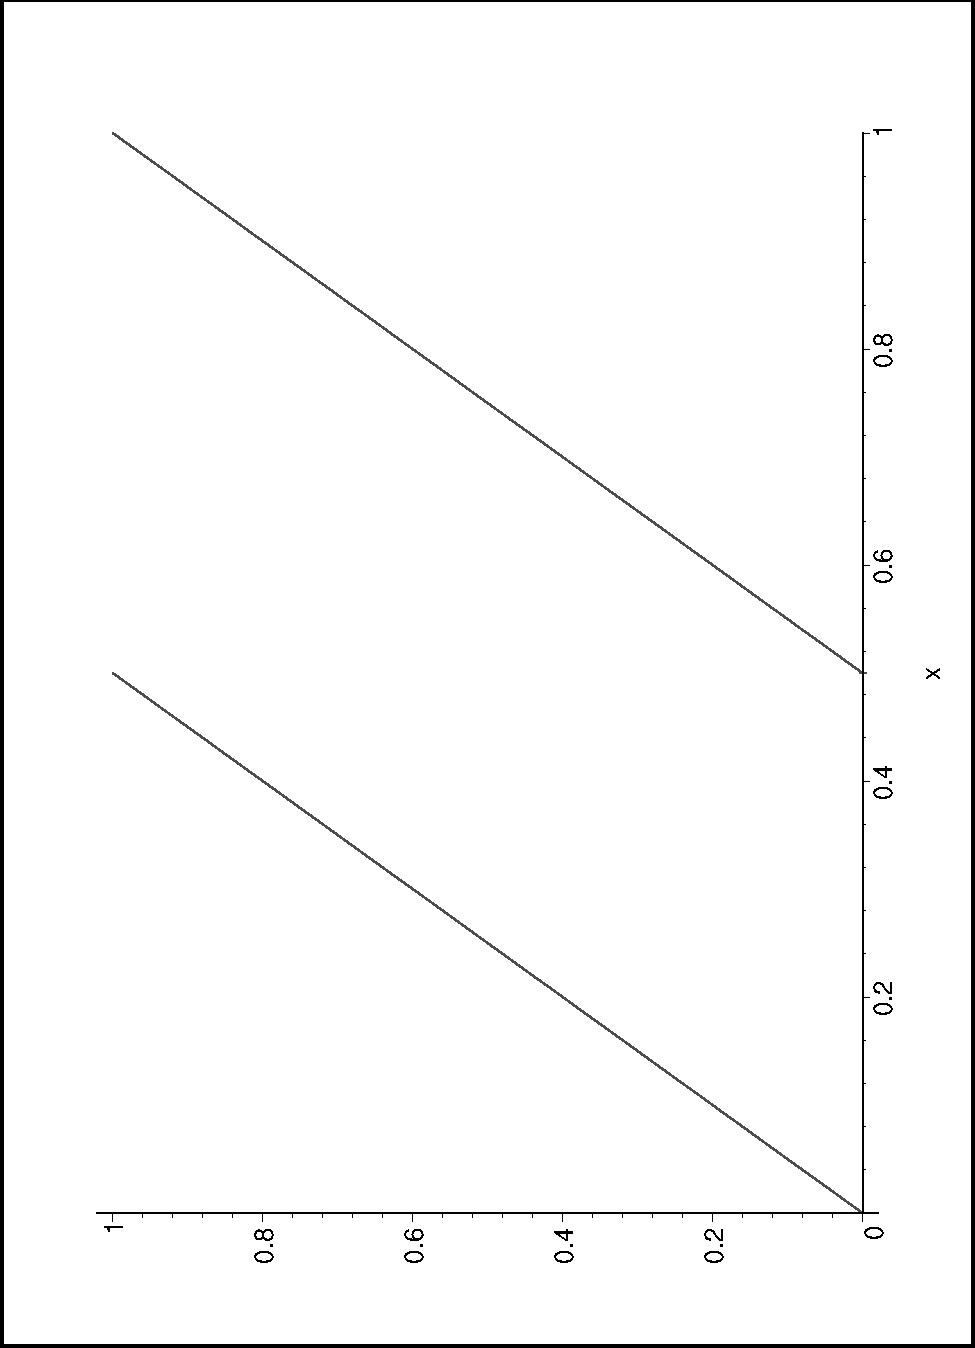
\includegraphics[angle=-90,scale=0.25]{graficas/r-ar}
        \end{center}
        \caption{Gr�fica de la transformacion 2-ardica, osea, $S(x)=2x (mod\;1)$}
    \end{figure}
    Se toma un intervalo $[0,x]\subset[0,1]$se calcula la imagen inversa de $[0,x]$ bajo $S$ la cual viene dada por:

    $$S^{-1}([0,x])=\cup_{i=0}^{r-1}{\Big[\frac{i}{r},\frac{i}{r}+\frac{x}{r}\Big]}$$

    Y calculando el Operador de Perron-Frobenius

    \begin{equation}
        \Pm f(x)=\frac{d}{dx}\sum_{i=0}^{r-1}{\int_{\frac{i}{r}}^{\frac{i}{x}+\frac{x}{r}}{f(u)du}}=
        \frac{1}{r}\sum_{i=0}^{r-1}{f\Big(\frac{i}{r}+\frac{x}{r}\Big)}
    \end{equation}
    Ahora como $r=2$ entonces $i$ toma valores de 0 e 1. Observando la grafica podemos concluir que
    $\frac{1}{2}\sum_{i=0}^2{f(\frac{i}{2}+\frac{x}{2})}=-\frac{1}{2}+\frac{1}{2}=0$ y por lo tanto
    $\Pm f(x)=0\; \forall x\in [0,1)$ pero $f(x)\neq 0$ para ningun $x\in[0,1]$.

La generalizaci�n inmediata de \eqref{c2n1} se tiene al extender $\X$ al plano $R^2$. Sea $A=[a,x]\times[b,y]$ entonces de \eqref{c2n0} se tiene
\begin{align*}
	\int_a^x{ds\int_b^y{\Pm f(s,t)dt}}&=\iint_{S^{-1}([a,x]\times[b,y])}{f(s,t)ds dt}\\
    \intertext{diferenciando con respecto a $x$ y luego con respecto a $y$, se tiene inmediatamente que}
    \Pm f(x,y)&=\frac{\partial^2}{\partial y\partial x}\iint_{S^{-1}([a,x]\times[b,y])}{f(s,t)ds dt}\\
    \intertext{y formulas an�logas que pueden derivarse en el caso de $\X\subset\R^d$}
\end{align*}

En el caso general, donde $\X=R^d$ y $S:\X\cir$ invertible, se puede derivar una interesante y �til generalizaci�n de
 la ecuaci�n \eqref{c2n1}. Para hacer esto primero se probar� el teorema del cambio de variable basado en el teorema de Radon-Nikodym.

\begin{dfn}(Funci�n de integraci�n acotada) Es una funci�n $f\in L^1\cap L^\infty$.
\end{dfn}

\begin{teo} Sea $(\X,\A,\mu)$ un espacio de medida, f de integraci�n acotada y una transformaci�n $S:\X\cir$ entonces para cada $A\in\A$
$$\int_{S^{-1}(A)}{f(S(x))\mu(dx)}=\int_{A}{f(x)\mu S^{-1}(dx)}=\int_A{f(x)J^{-1}(x)\mu(dx)}$$
Donde $\mu S^{-1}$ denota la medida
$$\mu S^{-1}(B)=\mu(S^{-1}(B))\qquad \text{B }\in\A$$
Y $J^{-1}$ es la densidad de $\mu S^{-1}$ con respecto a $\mu$, esto es,
$$\mu(S^{-1}(B))=\int_B{J^{-1}(x)\mu(dx)}\qquad \text{para } B\in\A $$
\end{teo}

\subparagraph{Observaci�n} Se usar� la notaci�n $J^{-1}(x)$ para mostrar la conexi�n con las transformaciones invertibles y
diferenciables de $\R^d$, en este sentido $J(x)$ es el determinante de la matriz del Jacobiano:
$$J(x)=\Big|\frac{dS(x)}{dx}\Big|\qquad o \qquad  J^{-1}(x)=\Big|\frac{dS^{-1}(x)}{dx}\Big|$$

\begin{proof}Obs�rvese que si tomamos $f(x)=1_B(x)$ entonces
\begin{align*}
f(S(x))=1_B(S(x))&=\begin{cases}
  				      1 & \text{si $B\in(S(x))$}\\
				      0 & \text{en otro caso}
                   \end{cases} \\
                 &=\begin{cases}
  					  1 & \text{si $S^{-1}(B)\in x$}\\
					  0 & \text{en otro caso}
                    \end{cases}\\
                 &= 1_{S^{-1}(B)}(x)
\intertext{y, por lo tanto}
\int_{S^1(A)}{f(S(x))\mu(dx)}&=\int_\X{1_{S^{-1}(A)}(x)f(S(x))\mu(dx)}\\
                             &=\int_\X{1_{S^{-1}(A)}(x)1_{S^{-1}(B)}(x)\mu(dx)}\\
                             &=\mu(S^{-1}(A)\cap S^{-1}(B))\\
                             &=\mu(S^{-1}(A\cap B))
\intertext{para la segunda integral del teorema se tiene}
\int_A{f(x)J^{-1}(x)\mu(dx)}&=\int_A{1_B(x)J^{-1}(x)\mu(dx)}\\
                            &=\mu(S^{-1}(A\cap B))
\intertext{la tercera integral toma la forma de}
\int_A{f(x)J^{-1}(x)\mu(dx)}&=\int_A{1_B(x)J^{-1}(x)\mu(dx)}\\
                            &=\int_{A\cap B}{J^{-1}(x)\mu(dx)}\\
                            &=\mu(S^{-1}(A\cap B))
\end{align*}

Ahora, se procede a probar para una funci�n simple $f(x)=\sum_{i=1}^{n}{\lambda_i 1_{B_i}(x)}$
\begin{align*}
f(S(x))=\sum_{i=1}^{n}{\lambda_i 1_{B_i}(S(x))}&=\begin{cases}
  				                   \sum_{i=1}^{n}{\lambda_i} & \text{si $B_i\in(S(x))$}\\
				                                           0 & \text{en otro caso}
                                                 \end{cases} \\
                                               &=\begin{cases}
  					               \sum_{i=1}^{n}{\lambda_i} & \text{si $S^{-1}(B_i)\in x$}\\
					                                       0 & \text{en otro caso}
                                                 \end{cases}\\
                 &= \sum_{i=1}^{n}{\lambda_i 1_{S^{-1}(B_i)}(x)}
\intertext{y, por lo tanto}
\int_{S^1(A)}{f(S(x))\mu(dx)}&=\int_\X{1_{S^{-1}(A)}(x)f(S(x))\mu(dx)}\\
                             &=\int_\X{1_{S^{-1}(A)}(x)\sum_{i=1}^{n}{\lambda_i 1_{S^{-1}(B_i)}(x)}\mu(dx)}\\
                             &=\sum_{i=1}^{n}{\lambda_i\int_\X{1_{S^{-1}(A)}(x) 1_{S^{-1}(B_i)}(x)}\mu(dx)}\\
                             &=\sum_{i=1}^{n}{\mu(S^{-1}(A)\cap S^{-1}(B_i))}\\
                             &=\mu(S^{-1}(A\cap B))
\intertext{para la segunda integral del teorema se tiene}
\int_A{f(x)J^{-1}(x)\mu(dx)}&=\int_A{\sum_{i=1}^{n}{\lambda_i 1_{B_i}(x)}J^{-1}(x)\mu(dx)}\\
                            &=\sum_{i=1}^{n}{\lambda_i \int_A{1_{B_i}(x)}J^{-1}(x)\mu(dx)}\\
                            &=\sum_{i=1}^{n}{\mu(S^{-1}(A)\cap S^{-1}(B_i))}\\
                            &=\mu(S^{-1}(A\cap B))
\intertext{la tercera integral toma la forma de}
\int_A{f(x)J^{-1}(x)\mu(dx)}&=\int_A{\sum_{i=1}^{n}{\lambda_i 1_{B_i}(x)}J^{-1}(x)\mu(dx)}\\
                            &=\sum_{i=1}^{n}{\int_{A}{\lambda_i 1_{B_i}J^{-1}(x)\mu(dx)}}\\
                            &=\sum_{i=1}^{n}{\int_{A\cap B_i}{J^{-1}(x)\mu(dx)}}\\
                            &=\sum_{i=1}^{n}{\mu(S^{-1}(A)\cap S^{-1}(B_i))}\\
                            &=\mu(S^{-1}(A\cap B))
\end{align*}
Como $f$ es una funci�n de integraci�n acotada podemos suponer que existe una sucesi�n $\{g_n\}$ de funciones simples
que convergen uniformemente a $f$. Por lo tanto, podemos evaluar los siguientes l�mites
\begin{align*}
\limi_{n\rightarrow\infty}\int_{S^1(A)}{g_n(S(x))\mu(dx)}&=\limi_{n\rightarrow\infty}\mu_n(S^{-1}(A\cap B))\\
                             &=\mu(S^{-1}(A\cap B))\\
\intertext{para la segunda integral del teorema se tiene}
\limi_{n\rightarrow\infty}\int_A{g_n(x)J^{-1}(x)\mu(dx)}&=\limi_{n\rightarrow\infty}\mu_n(S^{-1}(A\cap B))\\
                            &=\mu(S^{-1}(A\cap B))\\
\intertext{la tercera integral toma la forma de}
\limi_{n\rightarrow\infty}\int_A{g_n(x)J^{-1}(x)\mu(dx)}&=\limi_{n\rightarrow\infty}\mu_n(S^{-1}(A\cap B))\\
                            &=\mu(S^{-1}(A\cap B))
\end{align*}
\end{proof}

El teorema anterior es tomado por algunos autores como la definici�n del operador de Perron-Ruelle-Frobenius o operador de Transferencia.
El siguiente resultado es una consecuencia directa del teo (ref) y extiende la ecuaci�n (refe)

\begin{col} Sea $(\X,\A,\mu)$ un espacio de medida $S:\cir$ una transformaci�n no singular invertible y
$\Pm$ el operador de Perron-Frobenius asociado. Entonces para cada funci�n de integraci�n acotada, se tiene
$$\Pm f(x)=f(S^{-1}(x))J^{-1}$$
\end{col}

\begin{proof} Por la definici�n de $\Pm$, para $A\in\A$ se tiene
\begin{align*}
    \int_A{\Pm f(x)\mu(dx)}&=\int_{S^{-1}}{f(x)\mu(dx)}\\
    \intertext{Haciendo el cambio de variable en la integral con $y=S(x)$, tal que}
    \int_{S^{-1}(A)}{f(x)\mu(dx)}&=\int_A{f(S^{-1}(y))J^{-1}(y)\mu(dx)} \\
    \intertext{Por el teoremas \eqref{c2n00}}
    \int_A{\Pm f(x)\mu(dx)}&=\int_A{f(S^{-1}(x))J^{-1}(x)\mu(dx)} \\
    \intertext{Usando del teorema de Radon-Nikodym}
    \Pm f(x)&=f(S^{-1}(x))J^{-1}
\end{align*}
\end{proof}

\section{El operador de Koopman}

Se asume que $\mu$ es una medida. Se conoce que el siguiente diagrama conmuta

$$\begin{matrix}A\xrightarrow{\mu\circ S^{-1}}\mathbb{R}\\ S^{-1}\;{\searrow{\;\;}}\nearrow{\mu}\\  A\end{matrix}$$

Es decir $\nu=\mu\circ S^{-1}$ define una medida.  Si $\mu(A)=0$ entonces $\nu(A)=0$, entonces $\mu<<\nu$.La definici�n del
siguiente operador se basa en esta idea. Recu�rdese que $S:\X\cir$ y es suficiente tomar a $S$

\begin{dfn}[Operador de Koopman con respecto a S, $U$] El operador $U:L^{\infty}\rightarrow L^{\infty}$ se define como
    \begin{equation}
        Uf(x)=f(S(x)) \label{c2n3}
    \end{equation}
    Siendo $(\X,\A,\mu)$ un espacio de medida, $S:\X\cir$ una transformacion no-singular y $f\in L^{\infty}$.
\end{dfn}

\subparagraph{Observaci�n} $f_1(x)=f_2(x)\;\cs\Rightarrow f_1(S(x))=f_2(S(x))\;\cs $. En otras palabras,
$\mu(\{x:f_1(x)\neq f_2(x)\})=0$ entonces$\mu(\{x:f_1(S(x))\neq f_2(S(x))\})=0$ debido a
$\mu(\{ y:S(x)\in\{f_1(x)\neq f_2(x)\}\})= S\circ\mu(\{x:\{f_1(x)\neq f_2(x)\}\})=0$ por hip�tesis.
Por lo tanto el operador de koopman esta bien definido.

\paragraph{Propiedades del Operador de  Koopman}
    \begin{align}
        U(\lambda_1f_1+\lambda_2f_2)=\lambda_1Uf_1+\lambda_2Uf_2 && \forall f_1,f_2\in L^{\infty}, \lambda_1,\lambda_2\in\R  \\
        ||Uf||_{L^{\infty}}\leq ||f||_{L^{\infty}} && \text{Para cada $f\in L^{\infty}$} \\
        <\Pm f,g>=<f,U g> && \text{Para cada } f\in L^{\infty},g\in L^{\infty}
    \end{align}


\subparagraph{Observaci�n} La proposici�n expresa que $U$ es una contracci�n en $L^\infty$. De forma an�loga
que $U$ es el operador autoadjunto de $\Pm$ del operador de Perron-Frobenius.

\begin{proof} Para se tiene
    \begin{align*}
        U(\lambda_1f_1+\lambda_2f_2)(x)&=S(x)\circ(\lambda_1f_1+\lambda_2f_2)\\
                                       &=\lambda_1f_1(S(x))+\lambda_2f_2(S(x))\\
                                       &=\lambda_1Uf_1+\lambda_2Uf_2
    \end{align*}
    En el caso de se tiene
    $$|f(x)|\leq\sup_x\in\X|f(x)|=||f(x)||_{L^\infty}\cs$$
    por lo tanto $|f(S(x))|\leq||f||_{L^\infty}$
    Finalmente, para se asume que $g(x)=\car_A$ asi, en la primera parte de la ecuaci�n
    \begin{align*}
        <\Pm f,g>&=\int_\X{\Pm f(x)\car_A(x)\mu(dx)} \\
                 &=\int_X{\Pm f(x)\mu(dx)}
                   \begin{cases}
                    1 & \text{si $x\in A)$}\\
				    0 & \text{en otro caso}
                   \end{cases}\\
                 &=\int_A{\Pm f(x)\mu(dx)}
    \intertext{Ahora para el lado derecho de}
        <f,Ug>&=\int_X{f(x)U\car_A(x)\mu(dx)}\\
              &=\int_X{f(x)\car_A(S(x))\mu(dx)}\\
              &=\int_X{ f(x)\mu(dx)}
                   \begin{cases}
                    1 & \text{si $S(x)\in(A))$}\\
				    0 & \text{en otro caso}
                   \end{cases}\\
              &=\int_X{ f(x)\mu(dx)}
                   \begin{cases}
                    1 & \text{si $x\in S^{-1}(A))$}\\
				    0 & \text{en otro caso}
                   \end{cases}\\
              &=\int_{S^{-1}(A)}{ f(x)\mu(dx)}\\
    \intertext{Por lo tanto es equivalente a}
       \int_A{\Pm f(x)\mu(dx)}&=\int_{S^{-1}(A)}{ f(x)\mu(dx)}
    \intertext{La definici�n del operador de Perron-Frobenius.}
    \end{align*}
    Con lo cual para la funci�n caracter�stica. Supongamos $g(x)=\sum_{i=1}^n{\lambda_i\car_{A_i}(x)}$ asi,
     en la primera parte de la ecuaci�n
    \begin{align*}
        <\Pm f,g>&=\int_\X{\Pm f(x)\sum_{i=1}^n{\lambda_i\car_A(x)}\mu(dx)} \\
                 &=\sum_{i=1}^n{\lambda_i}\int_X{\Pm f(x)\mu(dx)}
                   \begin{cases}
                    1 & \text{si $x\in A_i$}\\
				    0 & \text{en otro caso}
                   \end{cases}\\
                 &=\sum_{i=1}^n{\lambda_i}\int_{A_i}{\Pm f(x)\mu(dx)}
    \intertext{Ahora para el lado derecho de }
        <f,Ug>&=\int_X{f(x)U\Big(\sum_{i=1}^n{\lambda_i\car_{A_i}(x)}\Big)\mu(dx)}\\
              &=\sum_{i=1}^n{\lambda_i}\int_X{f(x)\car_{A_i}(S(x))\mu(dx)}\\
              &=\sum_{i=1}^n{\lambda_i}\int_X{ f(x)\mu(dx)}
                   \begin{cases}
                    1 & \text{si $S(x)\in A_i$}\\
				    0 & \text{en otro caso}
                   \end{cases}\\
              &=\sum_{i=1}^n{\lambda_i}\int_X{ f(x)\mu(dx)}
                   \begin{cases}
                    1 & \text{si $x\in S^{-1}(A_i)$}\\
				    0 & \text{en otro caso}
                   \end{cases}\\
              &=\sum_{i=1}^n{\lambda_i}\int_{S^{-1}(A_i)}{ f(x)\mu(dx)}
    \end{align*}
    Con lo cual  para la una funci�n simple. Sea un sucesi�n $g=\{f_n\}$  que converge uniformemente a $f$. Entonces podemos evaluar el l�mite
    \begin{align*}
    \limi_{n\rightarrow\infty}<\Pm f,g_n>&=\limi_{n\rightarrow\infty}\int_\X{\Pm f(x) g_n\mu(dx)} \\
                 &=\int_A{\Pm f(x)\mu(dx)}
    \intertext{Ahora para el lado derecho de }
    \limi_{n\rightarrow\infty}<f,Ug_n>&=\limi_{n\rightarrow\infty}\int_X{f(x)U g_n\mu(dx)}\\
              &=\int_{S^{-1}(A)}{ f(x)\mu(dx)}
    \end{align*}
    Con lo que queda probado $ <\Pm f,g>=<f,U g>$.
\end{proof}

\begin{dfn}[Operador d�bilmente contin�o] Para cada sucesi�n $\{f_n\}$ contenida $L^{1}$ la condici�n $f_n\rightarrow f$
d�bilmente, implica $\Pm f_n\rightarrow \Pm f$ d�bilmente.
\end{dfn}

Con el operador de Koopman es f�cil probar el siguiente resultado

\begin{teo} El operador de Perron-Frobenius es d�bilmente continuo
\end{teo}

\begin{proof}Usando la propiedad  se puede mostrar que $<\Pm,g>=<f_n,g>$ para $g\in L\infty$. Como $<f_n,Ug>$
converge d�bilmente a $<f,Ug>$. Ahora  como $<f,Ug>=<\Pm,g>$ entonces   $<f_n,Ug>$ converge d�bilmente a $<\Pm,g>$. En consecuencia,
el operador de Perron-Frobenius es d�bilmente contin�o.
\end{proof}



\chapter{Estudio el Caos con Densidades}

Se introduce el concepto de medida invariantes por transformaciones, posteriormente, define e ilustra tres niveles de
irregularidades en el comportamiento de las transformaciones. Estos tres niveles son conocidos como ergodicidad, mezclante
(o mixing) y exactas. Asi mismo, se presentan sus caracterizaciones. El objetivo central del cap�tulo es mostrar la utilidad
de los operadores de Perron-Frobenius y Koopman en el estudio de de estos comportamientos.

Para una de densidad constante $f(x)=1$, preservar la medida es que sea una densidad estacionaria del operador de Perron-Frobenius,
osea, $\Pm 1=1$. Para la ergodicidad, la condici�n es que $f(x)=1$ sea la �nica densidad estacionaria para ese operador.
Finalmente, mixing y exacta son condiciones sobre la estabilidad de la densidad estacionaria.

\section{Medidas Invariantes}

\begin{dfn}(Medidas Invariantes Sobre $S$) Si $\mu(S^{-1}(A))=\mu(A)$ donde $S:\X\cir$ es una transformaci�n medible y $(\X,\A,\mu)$ un espacio de medida.
\end{dfn}

Observe que la preservaci�n de la medida depende de transformaci�n $S$ como de la  medida $\mu$. Esta relaci�n queda expl�cita cuando se dice que la medida $\mu$ es invariante bajo la transformaci�n $S$.

\begin{teo} Sea $(\X,\A,\mu)$ un espacio de medida, $S:\X\cir$ una transformaci�n no singular, y $\Pm$ el operador de Perron-Frobenius asociado con $S$.
Considere $f\in L^1$ entonces $\mu_f$ una medida dada por
\begin{equation}
\mu_f=\int_A{f(x)\mu(dx)}\label{c3n0}
\end{equation}
Es invariante si y solo si es un punto fijo de $\Pm$
\end{teo}

\begin{proof} Probemos las suficiencia de la propocici�n. Se asume la invarianza de la medida $\mu_f$. Entonces, por la definici�n de medida invariante se tiene
    \begin{align}
        \mu_f(A)&=\mu_f(S^{-1}(A))\qquad \forall A\in\A\nonumber\\
        \intertext{Lo cual por definici�n es}
        \int_A{f(x)\mu(dx)}&=\int_{S^{-1}(A)}{f(x)\mu(dx)} \qquad \text{para } A\in\A\label{c3n1}\\
        \intertext{Sin embargo, por la definici�n del operador de Perron-Frobenius, se tiene}
        \int_{S^{-1}}{f(x)\mu(dx)}&=\int_A{\Pm f(x)\mu(dx)}\qquad \text{para } A\in\A\label{c3n2}\\
        \intertext{Comparando \eqref{c3n1} con \eqref{c3n2} se tiene que}
        \int_A{f(x)\mu(dx)}&=\int_A{\Pm f(x)\mu(dx)}\nonumber\\
        \intertext{por lo tanto}
        f=\Pm f\nonumber
\end{align}
Si $\Pm f=f$ para algun $f\in L^1\;\geq 0$ entonces, se tiene
\begin{align*}
    f&=\int_A{f\mu(dx)}\\
     &=\mu_f(A)        \\
     &=\Pm f           \\
     &=\int_{S^{-1}(A)}{f\mu(dx)}\\
     &=\mu_f(S^{-1}(A)) \\
\intertext{Por lo tanto, se tiene que}
\mu_f(A)&=\mu_f(S^{-1}(A))
\end{align*}
Y por tanto, $S$ preserva la medida.
\end{proof}

\subparagraph{Observaci�n} La medida  es invariante sii $\Pm1=1$

\begin{ejm} Considere la transformaci�n r-ardica, presentada en el ejemplo \eqref{rardica}
$$S(x)=rx\qquad (mod 1)$$
donde $r>1$ es un entero. Recordemos que para $[0,x]\subset[0,1]$ se tiene que
    $$S^{-1}([0,x])=\cup_{i=0}^{r-1}{\Big[\frac{i}{r},\frac{i}{r}+\frac{x}{r}\Big]}$$
El operador de Perron-Frobenius para esta transformaci�n esta definido como
        $$\Pm f(x)=\frac{1}{r}\sum_{i=0}^{r-1}{f\Big(\frac{i}{r}+\frac{x}{r}\Big)}$$
asi
$$\Pm 1=\frac{1}{r}\sum_{i=0}^{r-1}{1}=1$$

Asi la funci�n 1 es un punto fijo, debido al teorema ?? transformaci�n r-ardica es invariante.

\end{ejm}


\section{Transformaciones Erg�dicas}

Que el operador de Frobenius-Perron $\Pm$ asociado a $S$ tenga una �rbita estacionaria. O equivalentemente, Que una transformaci�n $S$ tenga una medida invariante, no implica que $S$ tenga propiedades estad�sticas interesantes. Por ejemplo, si $S$ es la identidad sobre $\X$, �sea, $S(x)=x$ para todo $x\in \X$ entonces

Para todo $A\subset\X$, y, en consecuencia, $\Pm f=f$ para todo $f\in L^1$. Y claramente, estas transformaci�n no es interesante.
Sin embargo, si se mantiene para un subconjunto A de  $\X$, entonces la transfomaci�n puede ser estudiada separadamente sobre los conjuntos A o su complemento. Considerando las orbitas de $x^0$ la ecuaci�n implica que los elementos de A son mapeados en s� mismo y que ning�n elemento del complemento son mapeados en A. Un conjunto invariante que cumpla la condici�n anterior  necesariamente modulo cero,  motiva la siguiente definici�n.

\begin{dfn}[Transformaciones Erg�dicas] Si para cada conjunto invariante $A\in\A$ se cumple $\mu(A)=0$ o $\mu(\X\backslash\A)$
\end{dfn}

\subparagraph{Observaci�n} Si $S$ es erg�dica se dice que todos los conjuntos invariantes son subconjuntos \emph{triviales} de $\X$.

\begin{teo} Sea $(\X,\A,\mu)$ un espacio de medida y $S:\X\cir$ una transfomaci�n no singular. S es ergodico si y solo si, para cada
funci�n medible $f:\X\rightarrow\R$,
    \begin{equation}
        f(S(x))=f(x)\qquad \text{para casi todos los }x\in\X
    \end{equation}
Implica que f es constante $\cs$
\end{teo}

\begin{proof} Probemos que ergodicidad implica $f$ es constante. Se asume que $f$ no es una funci�n contante. Sea un numero real $r$ tal que
$r\in[a,b]$ donde $a$ y $b$ son el minimo y maximo de $S$. Entonces, existe algun r tal que
$$A=\{ x:f(x)\leq r\}\quad\text{y}\quad B=\{x:f(x)>\}$$
que tiene medida positiva. Observese que $\X=A\cup B$ y que los conjuntos son invariantes debido a
    \begin{align*}
        S^{A}&=\{x:S(x)\in A\}\\
             &=\{x:f(S(x))\leq r\}\\
             &=\{x:f(x)\leq r\}\\
             &=A\\
         \intertext{De modo similar para B}
         S^{B}&=\{x:S(x)\in B\}\\
             &=\{x:f(S(x))> r\}\\
             &=\{x:f(x)> r\}\\
             &=B\\
    \end{align*}
    Como los conjuntos $A$ y $B$ son invariantes y tiene medida positiva ambos conjuntos, $S$ no es erg�dico. Por lo tanto se tiene una contradici�n
    derivada de suponer que $f$ no es constante.
    Se probara la implicaci�n inversa. Se asume que S no es erg�dico, por lo tanto debe de existir un conjunto no-trivial que sea invariante. Siendo $f=\car_A$ y como A es no-trivial entonces f no es un funci�n constante. Sin embargo, como $A=S^{-1}(A)$ se tiene
    \begin{align*}
        f(S(x))&=1_A(S(x))\\
               &=\begin{cases}
                    1 & \text{si $A\in S(x)$}\\
                    0 & \text{si no}
                 \end{cases}\\
               &=\begin{cases}
                    1 & \text{si $S^{-1}(A)\in x$}\\
                    0 & \text{si no}
                 \end{cases}\\
               &=1_{S^{-1}(A)}(x)\\
               &=1_A(x)\\
               &=f(x)\;\cs
    \end{align*}
\end{proof}

\begin{teo} Sea $(\X,\A,\mu)$ un espacio de medida, $S:\cir$ una transformaci�n no sigunlar y $\Pm$ el operador de Perron-Frobenius asociado a $S$.
Si $S$ es erg�dico, entonces existe a lo sumo una densidad estacionaria $f_*$ de $\Pm$ y $f_*(x)>0\;\cs$ entonces $S$ es erg�dico. Adicionalmente,
Si existe una unica densidad estacionaria $f_*$ de $\Pm$ y $f(x)>0\;\cs$ entonces $S$ es ergodico.
\end{teo}

\begin{proof} Asuminos que $S$ es erg�dico y que $f_1$ y $f_2$ son 2 diferentes densidades estacionaria de $\Pm$. Si $g=f_1-f_2$ entonces
por la linealidad de $\Pm$ se tiene $\Pm g=g$. Por lo tanto, el teorema \ref{teopro} $g^+$ y $g^-$ ambas son densidades estacionarias de $\Pm$
    \begin{equation}
        \Pm g^+=g^+\qquad y \qquad \Pm g^-=g^-\label{elteopro}
    \end{equation}
  Por hip�tesis, $f_1$ y $f_2$ no solo son diferentes tambi�n son densidades por lo tanto
  $$g^+\neq 0\quad y \quad g^-\neq 0$$
  Los conjuntos
  $$A=\so g^+=\{x:g^+(x)>0\}$$
  y
  $$B=\so g^+=\{x:g^-(x)>0\}$$
  Dado que $A$ es el soporte de la parte positiva de $g$ y $B$ el soporte de la parte negativa entonces su intercesi�n es vac�a. Por lo tanto, son conjuntos disjuntos y de medida positiva. Por la proposici�n \eqref{elteopro} se tiene.
    $$A\subset S^{-1}(A)\qquad y \qquad B\subset S^{-1}(B)$$
    Como $A$ y $B$ son conjuntos disjuntos entonces $S^{-1}(A)$ y $S^{-1}(B)$ son disjuntos tambi�n. Por lo tanto aplicando sucesivamente REFE se tiene
    $$A\subset S^{-1}(A)\subset S^{-2}(A)\ldots\subset S^{-n}(A)$$
    Y
    $$B\subset S^{-1}(B)\subset S^{-2}(B)\ldots\subset S^{-n}(B)$$
    Entonces, $S^{-n}(A)$ y $S^{-n}(B)$ son disjuntos para todo n. Ahora definimos dos conjuntos como
    $$\bar{A}=\cap_{n=0}^\infty(S^{-n}(A))\qquad y \qquad \bar{B}=\cap_{n=0}^\infty{S^{-n}(B)}$$
    Estos dos conjuntos $\bar(A)$ y $\bar(B)$ son disjuntos tambien. Adem�s son invariantes ya que
    $$S^{-1}(\bar{A})=\cap_{n=0}^\infty(S^{-n}(A))=\cap_{n=1}^\infty{S^{-n}(A)}=\bar{A}$$
    y
    $$S^{-1}(\bar{B})=\cap_{n=0}^\infty(S^{-n}(B))=\cap_{n=1}^\infty{S^{-n}(B)}=\bar{B}$$
    Ni $\bar{A}$ ni $\bar{B}$ son conjuntos de media cero ya que ni $A$ ni $B$ son de media cero. Por lo tanto $\bar{A}$ y $\bar{B}$ son conjuntos no-triviales; contradiciendo la ergodicidad de S. As� la primera parte de teorema queda probada.
    Se demostrar� la segunda porci�n del teorema, por hip�tesis $f_*>0$ es la �nica densidad que satisface $\Pm f_*=f_*$, pero como S no es erg�dico,
    entonces existe conjuntos no triviales tal que
    $$S^{-1}(A)=A$$
    y junto a $\X-A$
    $$S^{-1}(B)=B$$
    Con eso dos conjuntos $A$ y $B$ se puede escribir $f_*=\car_A f_*+\car_B f_*$ entonces
    $$\car_A f_*+\car_B f_*=\Pm(\car_A f_*)+\Pm(\car_B f_*)$$
    La funci�n $\car_B f_*$ es igual a cero en el conjunto $\X-B=A=S^{-1}(A)$. Entonces, por la proposici�n \eqref{c2n00} $\Pm(\car_B f_*)$ 
    es igual a cero en $B=\X-A$. Entonces la igualdad?? implica que
    $$\car_A f_*=\Pm(\car_A f_*) \quad y\quad \car_B f_*=\Pm(\car_B f_*)$$
    As� como $f_*$ es positivo en $A$ y en $B$, se puede reemplazar $\car_A f_*$ por $f_A=\car_A/||\car_A f_*||$ y 
    $\car_B f_*$ por $f_B=\car_A/||\car_B f_*||$ en el �ltimo para de ecuaciones obteniendo
    $$f_A=\Pm(f_A) \quad y\quad f_B*=\Pm(f_B)$$
    Esto implica que existen dos densidades estacionarias de $\Pm$, contradiciendo la hip�tesis por lo tanto si hay una �nica densidad 
    estacionaria $f_*$ de $\Pm$ entonces es erg�dica.       
\end{proof}

\begin{teo}[Teorema Birkhoff] Sea $(\X,\A,\mu)$ un espacio de medida, $S:\X\cir$ una tranformaci�n y $f:\X\rightarrow\R$ una funci�n integrable. Si la medida $\mu$ es invariante, entonces existe una funci�n integrable $f^*$ tal que
    \begin{equation}
        f^*(x)=\limi_{n\rightarrow\infty}{\frac{1}{n}\sum^{n-1}_{k=0}{f(S^(x))}}\qquad \text{para la mayor�a $x\in\X$}\label{c3n3}
    \end{equation}
\end{teo}

\begin{teo} Sea $(\X,\A,\mu)$ un espacio de medida finito y $S:\X\cir$ una transformaci�n invariante y erg�dica. Entonces, para cualquier $f$,
el promedio de $f$ sobre la trayectoria es igual al promedio de $f$ sobre todo el espacio casi seguramente. Eso es,
    \begin{equation}
        \limi_{n\rightarrow\infty}{\frac{1}{n}\sum_{k=0}^{n-1}{f(S^k(x))}}=\frac{1}{\mu(\X)}\int_\X{f(x)mu(dx)} \quad \cs\label{c3n4}
    \end{equation}
\end{teo}

\begin{proof} Del teorema \eqref{c3n3} que dice que $f^*$ es constante casi seguramente. Entonces, se tiene
\begin{align*}
    \int_\X{f^*(x)\mu(dx)}&=f^*\int_\X{\mu(dx)}\\
                          &=f^*\mu(\X)\\
                          &=\int_\X{f(x)\mu(dx)}
\end{align*}
 Despejando
 $$f^*(x)=\frac{1}{\mu(\X)}\int_\X{f(x)\mu(dx)}\quad \cs$$
\end{proof}

Una de la consecuencias m�s citadas de este teorema, se presenta a continuaci�n

\begin{col} Sea $(\X,\A,\mu)$ un espacio de media finito y una medida $S:\X\cir$ invariante y erg�dica. Entonces para cualquier conjunto $A\in \A$
$\mu>0$ y la mayor�a de los puntos $x\in\X$ la fracci�n de los puntos $\{S^k(x)\}$ en $A$ tal que $k\rightarrow\infty$ viene dado por $\mu(A)/\mu(\X)$
\end{col}\label{colpro}

\begin{proof} Usando la funci�n caracter�stica $\car_A$ de A, sobre la fracci�n de puntos de $\{S^k(x)\}$ en $A$ es
$$\limi_{n\rightarrow\infty}\sum_{k=0}^{n-1}{\car_A(S^k(x))}$$
Sin embargo de \eqref{c3n4} esto implica $\mu(A)/\mu(\X)$
\end{proof}

\begin{obs} El corolario \ref{colpro} traduce que cada conjunto de medida positiva es visitado una infinidad de veces por las iteraciones para casi todos los puntos $x\in\X$. Es un resultado caso especial del \textbf{Teorema de Recurrencia de Poicar�}
\end{obs}

\section{Transformaciones Mezclantes y Exactas}

\begin{dfn}[Transformaci�n Mezclante] Si $S$ cumple que
\begin{equation}
\limi_{n\rightarrow\infty}{\mu(A\cap S^{-n}(B))}=\mu(A)\mu(B)\qquad \text{para todo} A,B\in\A
\end{equation}
Siendo $(\X,\A,\R)$ es un espacio de medida probabilidad, y $S:\X\cir$ una transformaci�n que preserva la medida.
\end{dfn}

La definici�n de mezclante puede ser interpretada de la siguiente forma.  Los puntos que partieron en A y finalizar�n en B despu�s de n iteraciones su medida est� determinada por el producto de las medidas de A y de B. Adicionalmente, es independiente de la posici�n inicial de $A$ y de $B$ en $\X$.

\subparagraph{Observaci�n} Es f�cil de ver cualquier transformaci�n de mezclante esta deber� ser erg�dica. Se asume que
$B\in\A$ es un conjunto invariante, en que se cumple $B=S^{-1}(B)$ y,  a�n m�s, $B=S^{-n}(B)$  por inducci�n. Se toma $A=\X  $
para que $\mu(A\cap B)=\mu(A\cap S^{-b}(B))=0$. Sin embargo, de que debe tener
y por lo tanto es o bien 0 o 1, lo que demuestra la ergodicidad

\begin{dfn}[Transformaci�n Exactas] Si $S$ cumple que
\begin{equation}
\limi_{n\rightarrow\infty}{\mu(S^n(A))}=1 \qquad \hbox{para cada $A\in\A, \mu(A)>0$}  
\end{equation}
Siendo $(\X,\A,\R)$ es un espacio de medida probabilidad, y $S:\X\cir$ una transformaci�n que preserva la medida.
\end{dfn}

Para ejemplificar la diferencia entre los tipos de transformaci�n se procede a mostra las seis primeras iteraciones de un 
n�mero aleatorio de 1000 puntos distribuidos en el conjunto de $\X=[0,1]\times[0,1]$ 

{\bf Transformaci�n Erg�dica}
\begin{equation}
S(x,y)=(\sqrt{2}+x,\sqrt{3}+y)\quad (mod\; 1)\label{t.erg}
\end{equation}
{\bf Transformaci�n Mezclante}
\begin{equation}
S(x,y)=(x+y,x+2y)\quad (mod \;1)\label{t.mez}
\end{equation}
{\bf Transformaci�n Exacta}
\begin{equation}
S(x,y)=(3x+y,x+3y)\quad (mod \;1)\label{t.exa}
\end{equation}


\begin{figure}
    \begin{center}
        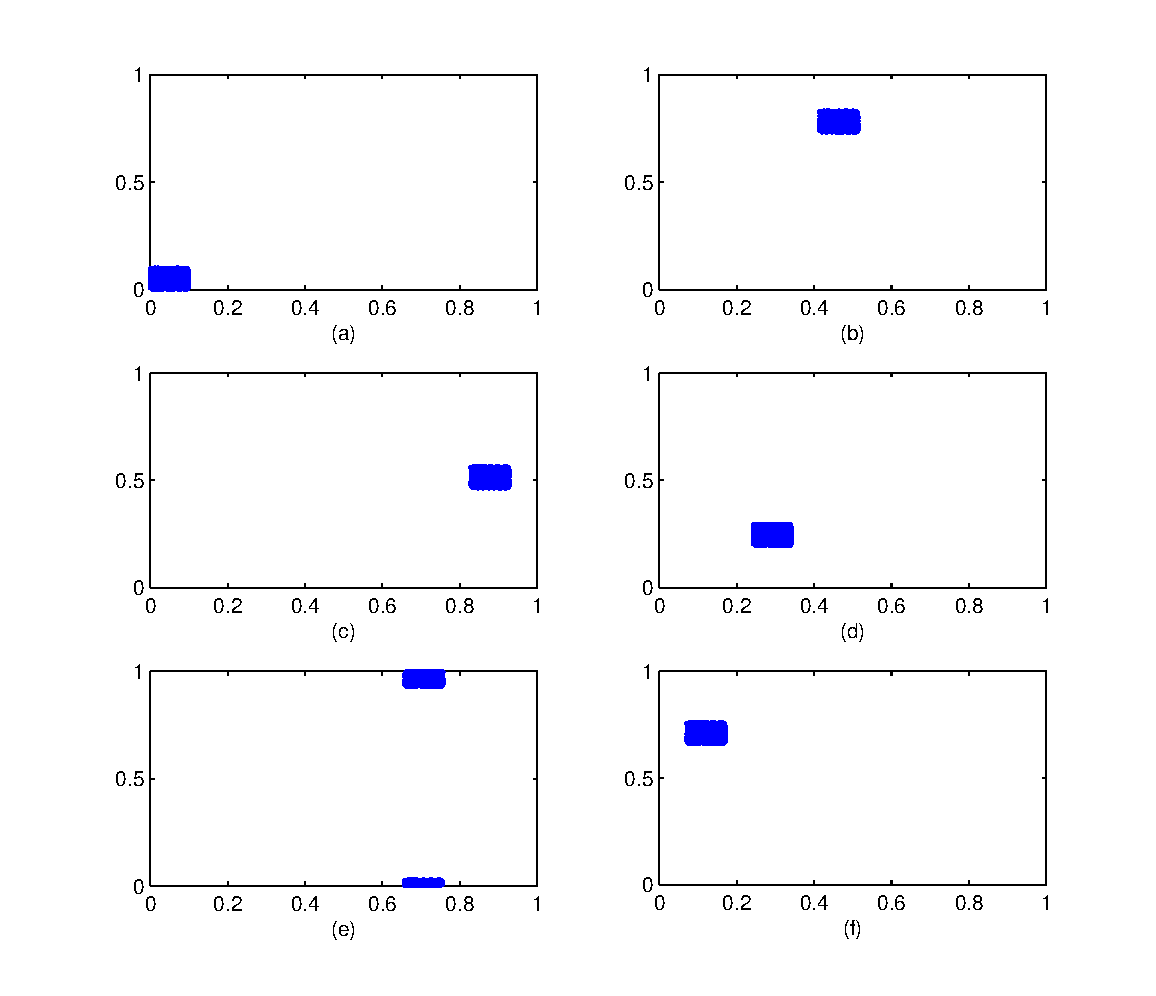
\includegraphics[width=.65\textwidth, height=1\textwidth,scale=0.5]{graficas/erg}
    \end{center}
    \caption{Iteraciones sucesivas de la transformaci�n \ref{t.erg}. Note como se mueve la distribuci�n de puntos en forma de cudrado sobre el espacio}

\end{figure}

\begin{figure}
    \begin{center}
        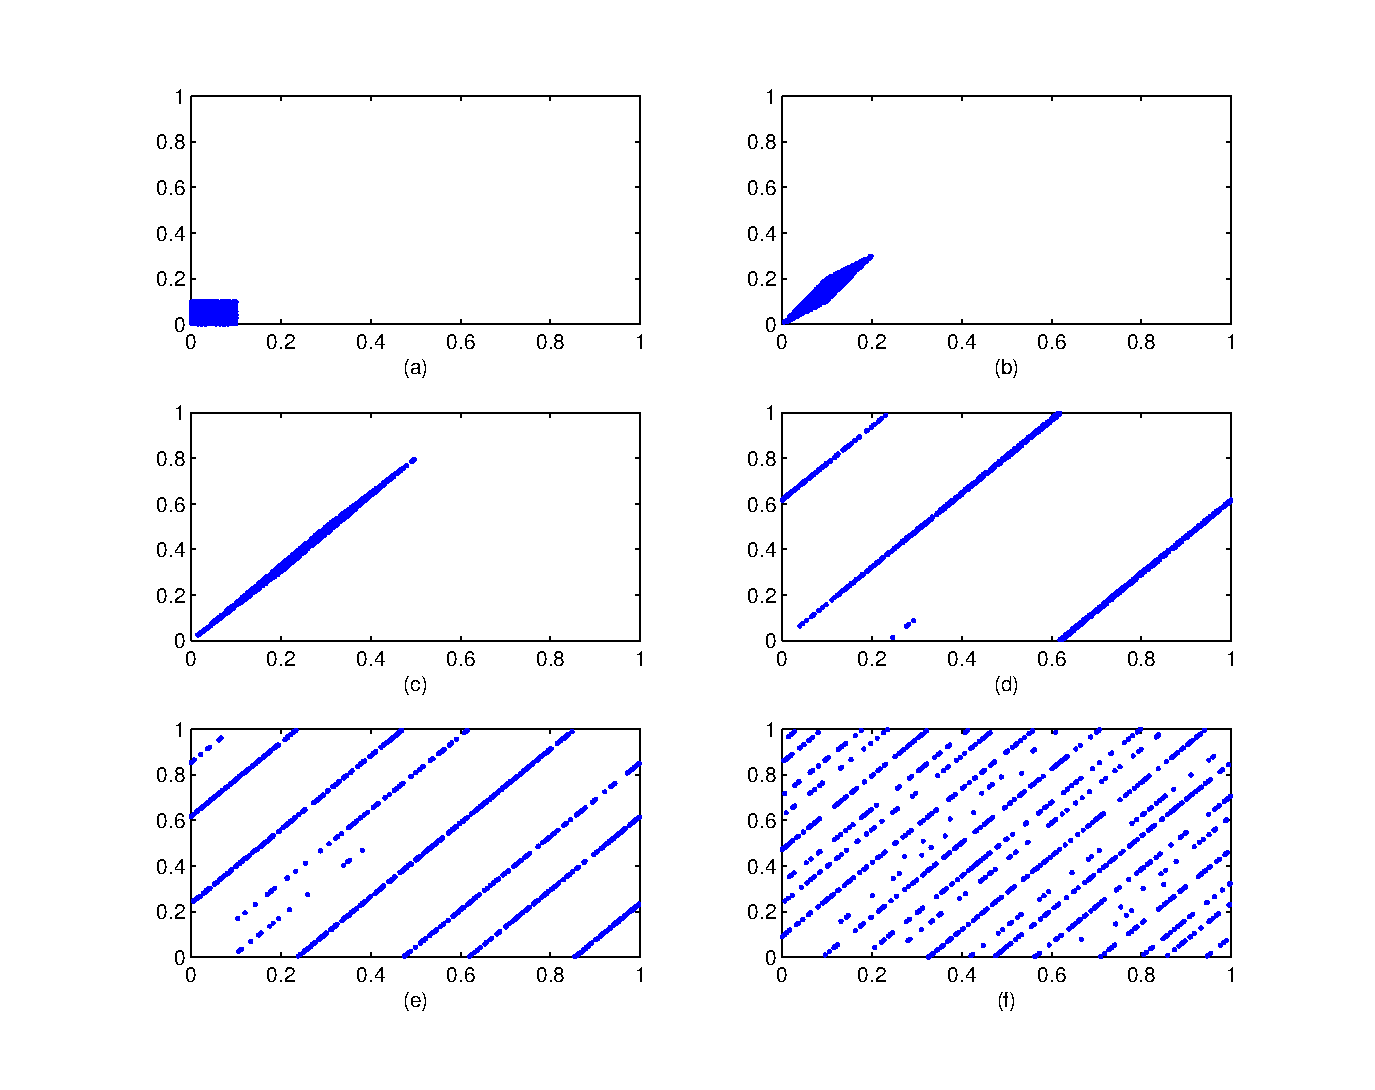
\includegraphics[width=.65\textwidth, height=1\textwidth,scale=0.5]{graficas/mix}
    \end{center}
    \caption{Iteraciones sucesivas de la transformaci�n \ref{t.mez}. Note como se esparce la distribuci�n de puntos sobre el espacio}

\end{figure}


\begin{figure}
    \begin{center}
        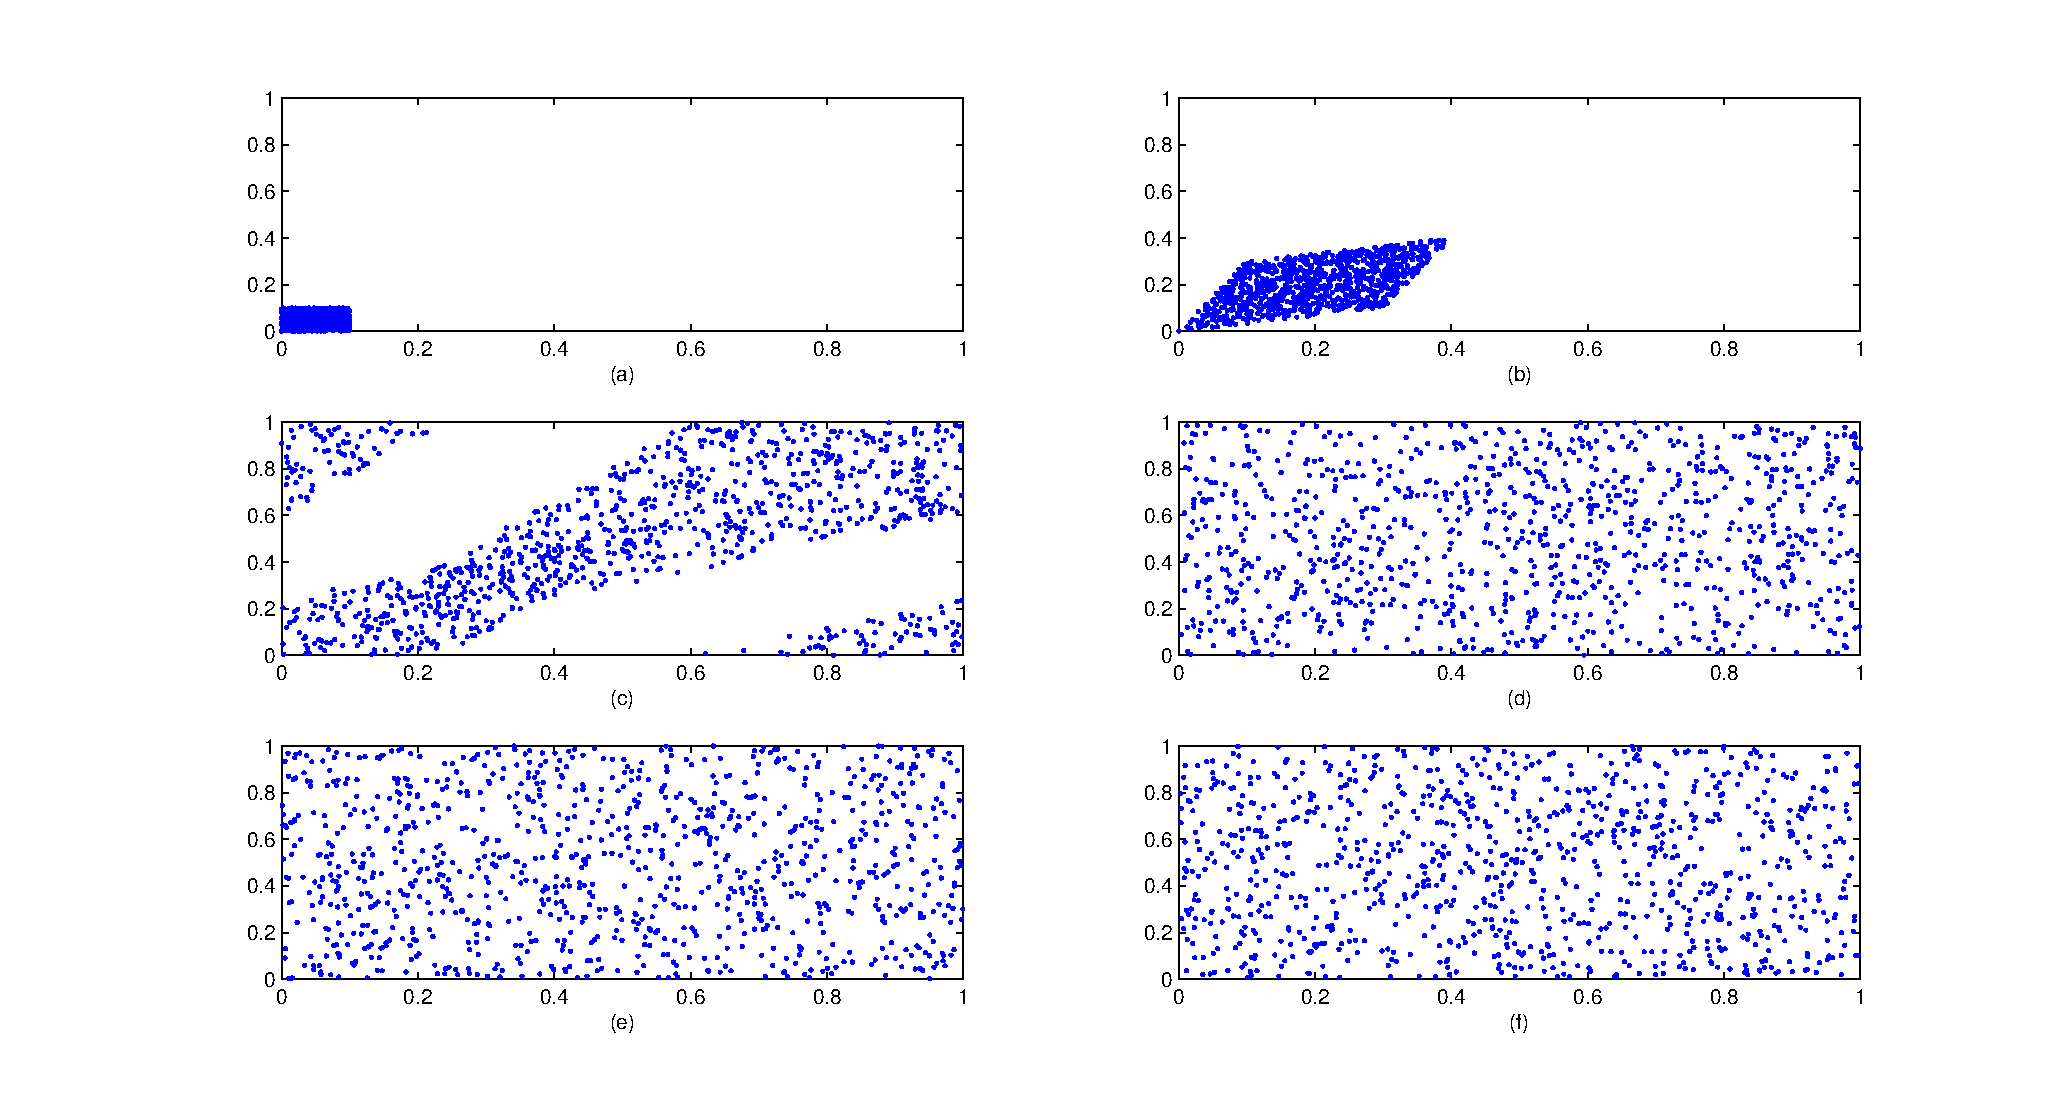
\includegraphics[width=.65\textwidth, height=1\textwidth,scale=0.5]{graficas/exa}
   \end{center}
    \caption{Iteraciones sucesivas de la transformaci�n \ref{t.exa}. Note como se esparce la distribuci�n de puntos sobre el espacio}

\end{figure}

\input{caos/usando/usando}



\chapter{Resultados Preliminares}

%En el cap�tulo anterior se dedic� a examinar los grados de "ca�tica" la conducta (ergodicidad, mezcla y exactitud)
%que preservan medida de las transformaciones puede mostrar. En particular, hemos visto la utilidad de la koopman y
%operadores de Frobenius-Perron para responder a estas preguntas.

%Teorem REFE reducido el problema de encontrar una medida invariante a una de hallar soluciones a la ecuaci�n f Pm = f.
%Tal vez la m�s obvia, aunque no el m�s simple, manera de encontrar estas soluciones es tomar un f arbitraria y examinar la secuencia
%{p} de sucesivas iteraciones de f por parte del operador de Frobenius-Perron. si {p} converge a f *, entonces es claro que {} = {}
%converge al mismo tiempo para f * y * Pf y ya est�. Sin embargo, para probar que {Pf} converge d�bilmente (o muy) a una funci�n f * es dificil.

%En este cap�tulo examinaremos en primer lugar la convergencia de la sucesi�n {AF} de promedios definidos por

%y mostrar c�mo esto puede ser usado para demostrar la existencia de una densidad estacionaria de P. A continuaci�n, muestran que bajo
%condiciones certin {Pf} puede mostrar una propiedad nueva, a saber, la periodicidad asint�tica. Por �ltimo, se introduce el concepto
%de estabilidad asint�tica para los operadores de Markov, que es una generalizaci�n de exactnes de Perron-Frobenius operadores. que la
%muestran como la tecnica funci�n de l�mite inferior se puede utilizar de demostrar estabilidad asint�tica. esta t�cnica es el uso en
%todo el resto del libro

\section{Funciones de Variaci�n Acotada}

\begin{dfn}[Valor medio de $f$, $m(f)$] Se define como
$$m(f)=\frac{1}{b-a}\int^b_a{f(x)dx}$$
De una funci�n $f:[a,b]\rightarrow\R$ real.
\end{dfn}

\begin{dfn}[Varianza, $D^2(f)$] Se define como
$$D^2(f)=m\Big((f-m(f))^2\Big)$$
\end{dfn}

%Ahora analicemos los inconvenientes de las definiciones precedentes. Consid�rese una sucesi�n %de funciones
%$\{ f_n\}$ definida como $f_n(x)=\sin{2n\pi x}\quad n=1,2,\ldots$.

\begin{dfn}[Variaci�n acotada,$s_n(f)$]  Se define como
    \begin{equation}
        s_n(f)=\sum^n_{i=1}{|f(x_i)-f(x_{i-1})|}
    \end{equation}
    Siendo f una funci�n real definida en el intervalo $\tri\subset\R$ y sea $[a,b]$ un subintervalo de
    $\tri$. As� mismo, considerando la partici�n de $[a,b]$ dada por
    \begin{equation}
        a=x_0<x_1<\ldots<x_n=b
    \end{equation}
    En donde todas las posibles sumas $s_n(f)$, corresponden a todas la divisiones de $[a,b]$, son acotadas por
     un n�mero que no depende de la subdivisi�n.
\end{dfn}

\begin{dfn}[Variaci�n Total,$\bigvee f(x)$]\label{variacionTotal} Se define como
    \begin{equation}
        \bigvee_a^b{f}=\sup{s_n(f)}
    \end{equation}
    donde el supremo se toma sobre todas la posibles particiones de la forma
\end{dfn}

\begin{ejm}Se asume que $f$ es una funci�n monotona, osea, creciente o decreciente. Entonces
$$|f(x_i)-f(x_{i-1})|=\theta[f(x_i)-f(x_{i-1})]$$
donde
\begin{equation*}
    \theta=\begin{cases}
                1 & \text{para $f$ creciente.}\\
               -1 & \text{para $f$ decreciente.}
           \end{cases}
\end{equation*}
    y, en consecuencia
    \begin{align*}
    s_n(f)&=\sum_{i=1}^n\theta[f(x_i)-f(x_{i-1})]\\
          &=\theta\sum_{i=1}^n[f(x_i)-f(x_{i-1})]\\
          &=\theta[f(x_n)-f(x_0)]\\
          &=|f(b)-f(a)|
    \end{align*}
    por lo tanto, cualquier funci�n se define y mon�tona en un intervalo cerrado es de variaci�n acotada.
\end{ejm}

\paragraph{La Variaci�n de la Suma}

Sea $f$ y $g$ sea una variaci�n acotada sobre $[a,b]$. Entonces

\begin{align*}
    s_n(f+g)&=\sum_{i=1}^n{{|f(x_i)+g(x_i)-[f(x_{i-1})+g(x_{i-1})]|}}                  \\
            &=\sum_{i=1}^n{|[f(x_i)-f(x_{i-1})]+[g(x_i)+g(x_{i-1})]|}                  \\
            &\leq\sum_{i=1}^n{\leq |f(x_i)-f(x_{i-1})|}+\sum_{i=1}^n{|g(x_i)-g(x_{i-1})|}  \\
            &  = s_n(f)+s_n(g)                                           \\
            &\leq \bigvee_a^b{f}+\bigvee_a^b{g}
\intertext{Y, en consecuencia}
\bigvee_a^b{(f+g)}&\leq\bigvee_a^b{f}+\bigvee_a^b{g}
\intertext{Si $f_1,\ldots,f_n$ es una variacion acotada sobre $[a,b]$, entonces por inducci�n argumento}
\end{align*}
\begin{equation}
    \bigvee_a^b{(f_1+\ldots+f_n)}\leq\bigvee_a^b{f_1}+\ldots+\bigvee_a^b{f_n}
\end{equation}
de deduce inmediatamente.
\paragraph{Variaci�n sobre la union de intervalo.}Se asume que $a<b<c$ y que la funci�n $f$ es una variaci�n
acotada sobre $[a,b]$ como tambi�n sobre $[b,c]$. Considere un porci�n de los intervalos
$[a,b]$ y $[b,c]$.
\begin{equation}
    a=x_0<x_1<\ldots<x_n=b=y_0<y_1<\ldots<y_m=c
\end{equation}
y las correspodientes sumas

$$\substack{s_n\\ [a,b]}(f)=\sum_{i=1}^n{|f(x_i)-f(x_{i-1})|}$$
$$\substack{s_n\\ [b,c]}(f)=\sum_{i=1}^m{|f(y_i)-f(y_{i-1})|}$$

Es evidente que la uni�n de la partici�n del intervalo de $[a,b]$. Entonces

\begin{equation}
    \substack{s_n\\ [a,b]}(f)+\substack{s_n\\ [b,c]}(f)=\substack{s_n\\ [a,c]}(f)
\end{equation}

Donde la parte del lado derecho de denota la suma correspondiente a la variaci�n de $f$ sobre
$[a,b]$. Observe que esta partici�n contiene un punto adicional, a saber b. Sin embargo, cualquier punto adicional
en la suma $s_n$ s�lo puede aumentar $s_n$, ya que estamos interesados en el supremo, esto es irrelevante.
De la ecuaci�n, se tiene

$$\bigvee_a^b{f}+\bigvee_b^c{f}=\bigvee_a^c{f}$$

Nuevamente usando inducci�n sobre el argumento en la �ltima f�rmula se tiene

\begin{equation}
    \bigvee_{a_0}^{a_1}{f}+\ldots+\bigvee_{a_{n-1}}^{a_n}{f}=\bigvee_{a_0}^{a_n}{f}
\end{equation}

donde $a_0<a_1<\ldots<a_n$ y $f$ es una variaci�n acotada sobre $[a_{i-1},a_i],\; i=1,\ldots,n$

\paragraph{Variaci�n de la composici�n de funciones} Sea $g:[\alpha,\beta]\rightarrow[a,b]$ es monotoma
creciente o monotoma decreciente sobre el intervalo $[\alpha,\beta]$ y sea $f:[a,b]\rightarrow\R$
 una funci�n dada. La composici�n $f\circ g$ esta bien definidad  para cualquier partici�n de $[\alpha, \beta]$
\begin{equation}
    \alpha=\sigma_0<\sigma_1<\ldots<\sigma_n=\beta
\end{equation}
la correspiente suma es

$$s_n(f\circ g)=\sum_{i=1}^n{|f(g(\sigma_i))-f(g(\sigma_i))|}$$

Observe que, debido a la monoton�a de $g$, la puntos $g(\sigma)$ definen una partici�n de $[a, b]$. As�
$s_n (f \circ g)$ es una suma determinada por la variaci�n de $f$ y, por lo tanto,

$$s_n(f\circ g)\leq \bigvee_a^b{f}$$

para cualquier partici�n. Consecuencia,

\begin{equation}
    \bigvee_\alpha^\beta{f\circ g}\leq\bigvee_a^b{f}.
\end{equation}

\paragraph{Variaci�n del Producto}Sea $f$ una variaci�n acotada sobre $[a,b]$ y sea la funci�n $g$ de clase $C^1$ sobre $[a,b]$. Entonces,

\begin{align*}
    s_n(fg)&=\sum_{i=1}^n{|f(x_i)g(x_i)-f(x_{i-1})g(x_{i-1})|} \\
           &=\sum_{i=1}^n{|f(x_i)g(x_i)-f(x_{i-1})g(x_{i-1})+f(x_i)g(x_{i-1})-f(x_i)g(x_{i-1})|}\\
           &=\sum_{i=1}^n{|f(x_i)g(x_i)-f(x_{i-1})g(x_{i-1})+f(x_{i-1})g(x_i)-f(x_{i-1})g(x_i)|}\\
           &=\sum_{i=1}^n{|g(x_i)\big(f(x_i)-f(x_{i-1})\big)+f(x_{i-1})\big(g(x_i)-g(x_{i-1})\big)|}\\
           &=\sum_{i=1}^n{|g(x_i)||f(x_i)-f(x_{i-1})|+|f(x_{i-1})||g(x_i)-g(x_{i-1}|}\\
\intertext{Aplicando el teorema del valor medio, se tiene}
           &\leq(\sup|g|)s_n(f)+\sum_{i=1}^n{|f(x_{i-1})g'(\tilde{x}_i)|(x_i-x_{i-1})} \\
           &\leq(\sup|g|)\bigvee_a^b f+\sum_{i=1}^n{|f(x_{i-1})g'(\tilde{x}_i)|(x_i-x_{i-1})}
\end{align*}

Con $\tilde{x}_i\in(x_{i-1}-x_i)$. Observe que el �ltimo t�rmino que se suma es una aproximaci�n de la integral de Riemann del producto $|f(x)g'(x)|$. As�, la variaci�n del producto $f(x)g(x)$ viene dada por la expresi�n
\begin{equation}
    \bigvee_a^b{fg}\leq(\sup|g|)\bigvee_a^b{f}+\int_a^b{|f(x)g'(x)|dx}
\end{equation}

En particular si $f=1$,

\begin{equation}
    \bigvee_a^b{g}\leq\int_a^b{|g'(x)|dx}
\end{equation}

Sin embargo, en el caso de $s_n$  entonces la igualdad es estricta  a la integral de Riemann de la integral de $g'$.

\paragraph{Desigualdad de Yorke} Sea $f$ definido en $[0,1]$ y sea de variaci�n acotada en $[a,b]\subset [0,1]$.
Se quiere evaluar la variaci�n del producto de $f$ y la funci�n caracter�stica $\car_[a,b]$. Sin p�rdida  de
generalidad, se asume que la partici�n del intervalo  $[0,1]$ siempre contiene los puntos $a$ y $b$. Entonces
\begin{align}
\substack{s_n\\ [0,1]}(f_n\car_{[a,b]})&\leq \substack{s_n\\ [a,b]}(f)+|f(a)|+|f(b)|\label{yorke1}\\
\intertext{Sea $c$ un arbitrario punto en $[a,b]$. Entonces, de la inecuaci�n anterior}
                                       &= \substack{s_n\\ [a,b]}(f)+|\big(f(b)-f(c)\big)+f(c)|+|\big(f(c)+f(a)\big)-f(c)|\nonumber\\
                                       &\leq \substack{s_n\\ [a,b]}(f)+|f(b)-f(c)|+|f(c)-f(a)|+2|f(c)|\nonumber\\
                                       &\leq 2\bigvee_a^b{f}+2|f(c)|\nonumber\\
\intertext{Siempre es posible elegir un punto $c$ tal que}
|f(c)|&\leq \frac{1}{b-a}\int_a^b{|f(x)|dx}\nonumber\\
\intertext{De modo que}
\substack{s_n\\ [a,b]}(f_n\car_{[a,b]})&\leq 2\bigvee_a^b{f}+\frac{2}{b-a}\int_a^b{|f(x)|dx}\nonumber
\end{align}
Entonces queda
\begin{equation}
    \bigvee_0^1{f\car_{[a,b]}}\leq 2\bigvee_a^b{f}+\frac{2}{b-a}\int_a^b{|f(x)|dx}
\end{equation}
\newpage

\section{Principio de Selecci\'on de Helly}

Antes de enunciar el principio de Helly, se probaran unos lemas que ser\'an utiles en la demostraci\'on del teorema de Lasota-Yoker.
\begin{lem} Si $f\in C^1[a,b]$ con $|f'(x)|>0$, entonces f es mon\'otona sobre $[a,b]$.
\end{lem}\label{lema01}

\begin{proof}Sea $f\in C^1[a,b] \Rightarrow f'\in C[a,b]$. Por hip\'otesis, $f'\in(-\infty,0)$ o $f'\in(0, \infty)$.
Y como $f'$ es continua, entonces solo es posible  $f'<0\; \forall x\in[a,b]$ o $f'>0\; \forall x\in[a,b]$, en otra palabra que $f'$ sea mon\'otona.
\end{proof}


\begin{lem}Sea $f$ un funci\'on diferenciable uno a uno, y sea $g=f^1$. Si $|f'|\geq\alpha$ entonces $|g'|\leq\frac{1}{\alpha}$
\end{lem}\label{lema05}

\begin{proof}Sea
\begin{align*}
    f(g(x))&=x\\
    f'(g(x))g'(x)&=1\\
    |f'(g(x))|&=\frac{1}{g'(x)}\\
              &\geq\alpha\\
\intertext{por lo tanto $|g'(x)|\leq\frac{1}{\alpha}$}
\end{align*}
\end{proof}

\begin{lem} Si $\bigvee_0^1{f}\leq a$ y $||f||\leq b$, donde $||f||=\int_0^1{|f|}$ entonces $|f(x)|\leq a+b$ $\forall x$ 
\end{lem}\label{lema07}

\begin{proof} Si $||f||\leq b\Rightarrow\exists\alpha$ tal que $|f(\alpha)|\leq b$. Si no, entonces $|f(x)|>b\;\forall x\in[0,1]$ 
y por lo tanto $\int_0^1{|f|}>\int_0^1{b}=b$ y tenemos una contradici\'on. Por lo tanto $|f(x)-f(\alpha)|\leq \bigvee_0^1{f}\leq a$
por lo tanto
$$|f(x)|-|f(\alpha)|\leq a$$
y $$|f(x)|\leq a+|f(\alpha)$$
$$|f(x)|\leq a+b$$
\end{proof}

\begin{teo}[Helly] Sea$\Fe$ una colecci\'on infinita de de funciones de variaci\'on acotada en un intervalo $[a,b]$ 
y supongamos que existe $K>0$ tal que 
$$|f(x)|\leq K\quad \bigvee_{[a,b]}{f}\leq K\quad \forall f\in \Fe$$
entonces existe una sucesi\'on $\{f_n\}\subset\Fe$ que converge a todo punto $x\in[a,b]$ a una funci\'on $f_*$ de variaci\'on acotada,
 tal que $\bigvee_{[a,b]}{f_*}\leq K$
\end{teo}\label{helly}


\section{Teorema de Mazur}

\begin{dfn}[Clausura,$\ov{E}$] Si $\ov{E}=\{x\in\X:\forall B(x,\epsilon)\cap E\neq\emptyset\}$
\end{dfn}

\begin{obs} Equivalentemente la clausura se puede definir mediante $\ov{E}=E\cup E'$ donde $E'$ es el conjunto de los puntos de acumulaci\'on de E. Tambi\'en, es la intersecci\'on de todos los conjuntos cerrados que contienen a E.
\end{obs}

\begin{dfn}[Totalmente acotado]  Si  $\forall \epsilon>0,\; \exists x_1,x_2,\ldots,x_n \in \X$ tal que
$\cup^n_{i=1}{B(x_i,\epsilon)}\supseteq\X$ siendo $(\X,d)$ un espacio m\'etrico.
\end{dfn}

\begin{obs} Se cumple que todo espacio totalmente acotado es tambi\'en acotado. Adem\'as, todo compacto es totalmente acotado.
Esta propiedad es \'util precisamente para demostrar compacidad, pues se tiene que existe equivalencia entre ser compacto
y ser totalmente acotado y completo.
\end{obs}

De hecho, para muchas demostraciones es precisamente \'esta caracterizaci\'on de compacidad la que se utiliza.

\begin{dfn}[Relativamente compacto] Si toda sucesi\'on de elementos de S tiene una subsucesi\'on que converge en X.
 Siendo $S$ un subconjunto de un espacio topol\'ogico $\X$
\end{dfn}

\begin{obs} Para espacios métricos tenemos definici\'on equivalente. A es relativamente compacto si y solo si su clausura es un compacto
\end{obs}

\begin{dfn}[Envolvente Convexa, co(A)] Es el conjunto de todas las combinaciones convexas de elementos de A, es decir, el conjunto de todas las sumas
$\sum^n_{i=1}{t_ix_i}$ donde $x_i\in A,\; t_i\geq 0,\; \sum{t_i}=1$ para un $n$ arbitrario.
\end{dfn}

\begin{teo}[Mazur] Sea $\X$ un espacio de banach con $A\subset\X$ es un compacto relativo, entonces $\ov{co}(A)$ es compacto.
\end{teo}\label{mazur}

\begin{proof} Por la definici\'on de espacio Banach, $\ov{co}(A)$ es completo asi que $co(A)\subset\X$. Por consiguiente, solo queda probar
que $co(A)$ es totalmente acotada.

Como $A$ es totalmente acotado entonces $\ov{A}$ es compacto. Adicionalmente, se escoje $\epsilon>0$, por lo tanto existe un subcojunto finito
$\{x_1,x_2,\ldots,x_n\}\subset A$ tal que
$$A\subset\cup^n_{i=1}{B(x_i,\frac{\epsilon}{4})}$$

Sea $B=co\{x_1,x_2,\ldots,x_n\}$ y note que (eso no lo entiendo)
$$\ov{co}(A)\subset\cup^n_{i=1}{B(co(A),\frac{\epsilon}{4})}$$

Sea $\upsilon:A\rightarrow\{1,2,\ldots,n\}$ tal que
$$g\in A\Rightarrow||g-x_{\upsilon(g)}||<\frac{\epsilon}{4}$$

Para $t\in co(A)$
$$t=\sum^m_{i=1}{a_it_i}$$
donde $t_i\in A$, $a_i\geq 0$ y $\sum^m_{i=1}{a_i}=1$

entonces
\begin{align*}
    ||t-\sum^m_{i=1}{a_ix_{\upsilon(t_i)}}||&=||\sum^m_{i=1}{a_i(t_i-x_{\upsilon(t_i))}}||\\
                                            &\leq \sum^m_{i=1}{|a_i| ||x_{\upsilon(t_i)}||}\\
                                            &\leq\frac{\epsilon}{4}
\end{align*}

Esto es para $t\in co(A)$
$$d(x,B)<\frac{\epsilon}{4}$$

En consecuencia, $co(A)\subset \cup^n_{i=1}{B(B,\frac{\epsilon}{4})}$ entonces
$\cup^n_{i=1}{B(co(A),\frac{\epsilon}{4})}\subset\cup^n_{i=1}{B(B,\frac{\epsilon}{4})}$
y por lo tanto $\ov{co}(A)\subset\cup^n_{i=1}{B(B,\frac{\epsilon}{2})}$

Ahora, la transformaci\'on
$$\mu:(a_1,a_2,\ldots,a_n,x_1,x_2,\ldots,x_n)\rightarrow\sum^{n}_{i=1}{a_ix_i}$$
es una transfomaci\'on continua de un conjunto compacto
$$[0,1]\times[0,1]\times\ldots\times[0,1]=\prod^n_{i=1}{x_i}\hbox{ sobre B}$$

En consecuencia, B es un compacto y por lo tanto es totalmente acotado. Entonces exiten $b_1,b_2\ldots b_n\in B$ tal que
$$B\subset \cup^n_{i=1}{B(b_i,\frac{\epsilon}{2})}$$.

Como $\ov{co}(A)\subset\cup^n_{i=1}{B(B,\frac{\epsilon}{2})}\subset\cup^n_{i=1}{B(b_i,\frac{\epsilon}{2})}$.
$\ov{co}(A)$ es totalmente acotado y por lo tanto es compacto

\end{proof}

 \newpage


\section{Teorema de Kakutani-Yosida}

En esta secci�n se revisar� algunas propiedades resaltantes de los promedios definidos como
\begin{equation}
A_n f=\frac{1}{n}\sum_{k=0}^{n-1}{\Pm f}\qquad f\in L^1
\end{equation}
Se asume que un espacio de medida $(\X,\A,\mu)$ y operador $\Pm:L^1\cir$ de Markov.
\begin{pro} Para todo $f\in L^1$
\begin{equation}
\limi_{n\rightarrow\infty}||A_nf-A_n\Pm f||=0\label{c4n1}
\end{equation}
\end{pro}

\begin{proof} Por definici�n del promedio $A_n f$ se tiene
\begin{align*}
    A_n f- A_n\Pm f   &=\Big(\frac{1}{n}\Big)\Big(\sum_{k=0}^{n-1}{\Pm f}-\sum_{k=0}^{n-1}{\Pm \Pm^{k_n}} f\Big)\\
                      &=\Big(\frac{1}{n}\Big)\sum_{k=0}^{n-1}{\Pm}(f -\Pm^{n} f)\\
\intertext{y por lo tanto}
    ||A_n f-A_n\Pm f||&=||\Big(\frac{1}{n}\Big)\sum_{k=0}^{n-1}{\Pm}(f -\Pm^{n} f)||\\
\intertext{es una proposici�n Markov elemental tal que $||\Pm^n f||\leq ||f||$ se tiene}
                      &\leq\Big(\frac{1}{n}\Big)||(f -\Pm^{n} f)||\\
                      &\leq \Big(\frac{1}{n}\Big)(||f||+||\Pm^n f||)\\
\intertext{usando nuevamente la propiedad contractiva}
    ||A_n f -A_n\Pm f||&\leq\Big(\frac{2}{n}\Big)||f||\rightarrow 0
\intertext{cuando $n\rightarrow\infty$, esto completa la prueba.}
\end{align*}

\end{proof}

Este resultado y el pr�ximo resultado son casos especiales del teorema de teorema abstracto Kakutani-Yosida. Aunque antes
se debe presentar la siguiente definici�n dual de convergencia en precompacto.

\begin{dfn} El conjunto $\Fe$ es llamado fuertemente o d�bilmente precompacto si cada sucesi�n de funciones
$\{f_n\},\;f_n\in\Fe$, contiene una subsecesi�n convergente fuertemente o d�bilmente $\{f_{\alpha_n}\}$ que converge a un
 $\overline{f}\in L^p$
\end{dfn}

\begin{pro} Si para $f\in L^1$ existe una subsucesi�n  $\{A_{\alpha_n}f\}$ de la sucesi�n $\{A_n f\}$ que converge
d�bilmente a $f_*\in L^1$, entonces $\Pm f_*=f_*$
\end{pro}\label{c4n2}

\begin{proof} Como $\Pm A_{a_n}f=A_{a_n}\Pm f$ entonces $\{A_{a_n}\Pm f\}$ converge d�bilmente a $\Pm f_*$.
Entonces $\{A_{a_n}\Pm f\}$ entonces tiene al mismo limite $\{A_{a_n}f\}$, Se tiene $\Pm f_*=f_*$
\end{proof}

\begin{teo}[Kakatani-Yosida] Sea $(\X,\A,\mu)$ un espacio de medida y $\Pm:\X\cir$ un operador de Markov. Si para una funcion dada $f\in L^1$
la sucesi�n $\{A_ f\}$ es d�bilmente precompacta, entonces esta converge fuertemente para alg�n  $f_*\in L^1$ que es un
punto fijo de $\Pm$, a saber, $\Pm f_*=f_*$. Adicionalmente, si $f\in D$, entonces$f_*\in D$, de modo que $f_*$ es una
densidad estacionaria.
\end{teo}

\begin{proof} Como $\{A_n f\}$ es debilmente precompacto, por hip�tesis, entonces una subsucesi�n $\{A_{n_k} f\}$ que converge d�bilmente
a algun $f_*\in L^1$. Ademas, por la proposici�n ?? se tiene que $\Pm f_*=f_*$
 
Se escribe $f\in L^1$ en la siguiente forma
\begin{align}
    f&=(f-f_*)+f_*\label{c4n3}\\
\intertext{Para un tiempo inicial se tiene que  para cualquie $\epsilon>0$ la funci�n $f-f_*$ puede ser escrita en la siguiente forma}
    f-f_*&=\Pm g-g+r\label{c4n4}\\
\intertext{donde $g\in L^1$ y $||r||<\epsilon$. Asi de las ecuaciones \eqref{c4n3} y \eqref{c4n4} se tiene}
    A_n f&=A_n(\Pm g-g)+A_n r+A_n f_*\nonumber\\
\intertext{Como $\Pm f_*=f_*$, $A_n f_*=f_*$ se obtiene}
     ||A_n f-f_*||&=||A_n(f-f_*)||\nonumber\\
                  &\leq||A_n(\Pm g-g)||+||A_n r||\nonumber\\
\intertext{Por la proposici�n \eqref{c4n1} se sabe que $||A_n(\Pm g-g)$ converge fuertemente a cero cuando n tiende a infinito
por hip�tesis $||A_n r||\leq||r||<\epsilon$. Entonces para un $n$ lo suficientemente largo se tiene}
    ||A_n f-f_*||&\leq\epsilon\nonumber
\end{align}
ya que $\epsilon$ es arbitrario, esto prueba que $\{A_n f\}$ converge fuertemente a $f_*$

Esto muestra que $f\in D$, entonces $f_*\in D$. Por efinicion $f\in D$ es $f\geq 0$ y $||f||=1$, entonces $\Pm f\geq 0$ y $||\Pm f||=1$
y por lo tanto $\Pm^n f \geq 0 y ||\Pm^n f||=1$. Por consecuencia $A_n f\geq 0$ y $||A_n f||=1$, como $\{A_n f\}$ converge 
fuertemente a $f_*$ se debe tener que $f_*\in D$. Se completo la demostraci\'on bajo la hip�tesis de que la representaci\'on \eqref{c4n4} 
siempre es posible para cualquier $\epsilon$. 

Para verificar esta suposicion, se usara la version simplificada del teorema de Hahn-Banach. Supongase que no existe un r tal que 
la ecuaci�n \eqref{c4n4} sea cierta. En ese caso entonces, $f-f_*\in ov{(P-I)}L^1(\X)$ y entonces, por el teorema de Hahn-Banach, se tiene que existe
$g_0\infty$ tal que
\begin{equation}
<f-f_*,g_0>\neq 0\label{c4n5}
\end{equation}
y
$$<h,g_0>=0\qquad \hbox{para todo $h\in\ov{(P-I)}L^1(\X)$}$$
en particular
$$<(\Pm-I)\Pm^j f, g_0>=0$$
Entonces 
$$<\Pm^{j+1}f,g_0>=<\Pm^j,g_0>\qquad j=0,1,\ldots$$
y por inducci�n se tiene
$$<\Pm^j f,g_0>=<f,g_0>$$
y en consecuencias
$$\frac{1}{n}\sum_{j=0}^{n-1}{<\Pm^j f,g_0>}=\frac{1}{n}\sum_{j=0}^{n-1}{<f,g_0>}=<f,g_0>$$ 
o
\begin{equation}
<A_n f,g_0>=<f,g_0>\label{c4n6}
\end{equation}
Como $\{A_{\alpha_n} f\}$ se asumio que converge d�bilemente a $f_*$, se tiene
$$\limi_n<A_{\alpha_n} f,g_0>=<f_*,g>$$
y por \eqref{c4n6}
$$<f,g_0>=<f_*,g_0>$$
es equivalente a 
$$<f-f_*,g_0>=0$$
Sin embargo, esto contradice \eqref{c4n5} por lo tanto se puede concluir que la representaci�n \eqref{c4n4} es siempre posible.
\end{proof}

El teorema anterior reduce el problema de la existencia de una densidad estacionaria $f_*$ para el operador
$\Pm$, es decir, $\Pm f_*=f_*$, Al problema de demostrar la precompacidad d�bil de la sucesi�n $\{A_n f\}$.
En el caso especial del operador $\Pm$ de Perron-Frobenius es suficiente demostrar la existencia de medidas invariantes.

\begin{col}Sea $(\X,\A,\mu)$ un espacio de medida y $\Pm:L^1\cir$ una operador de Markov. Si para alg�n $f\in D$ existe un $g\in L^1$ tal que
    \begin{equation}
        \Pm^n f\leq g
    \end{equation}
    Para toda n, entonces existe un $f_* \in D$ tal que $\Pm f_*=f_*$, es decir, $f_*$ es una densidad estacionaria.
\end{col}

\begin{proof} Por hip�tesis, $\Pm^n f\leq g$ entoces
$$0\leq A_n f=\frac{1}{n}\sum^{n-1}_{k=0}{\Pm^k f}\leq g$$
y, entonces, $|A_n f|\leq g$. Por el primer criterio de d�bilmente precompacto, entonces $\{A_n f\}$ es d�bilmente precompacto. Con
lo cual se concluye el argumento.
\end{proof}

\begin{col} ea $(\X,\A,\mu)$ un espacio de medida y $\Pm:L^1\cir$ un operador de Markov. Si para alg�n $f\in D$ existe $M>0$ y $p>1$ tal que
    \begin{equation}
        ||\Pm^n f||_{L^p}\leq M
    \end{equation}
    Para todo n, entonces existe un $f_*\in D$ tal que $\Pm f_*=f_*$
\end{col}

\begin{proof} Se tiene
    \begin{align*}
            ||A_n f||_{L^p}&=\big||\frac{1}{n}\sum^{n-1}_{k=0}{\Pm^k f}\big||_{L^p}\\
                       &\leq\frac{1}{n}\sum^{n-1}_{k=0}{||\Pm^k f||_{L^p}}\\
                       &\leq\frac{1}{n}(nM)\\
                       &=M
    \end{align*}
    Se tiene  por el segundo criterio de precompacto, $\{A_n f\}$ es d�bilmente precompacto.
\end{proof}

%\begin{teo} Sea $(\X,\A,\mu)$ un espacio de medida y $\Pm:L^1\cir$ un operador de Markov junto a la �nica densidad estacionaria
%$f_*$. Si $f_*(x)>0$ para todo $x\in\X$, entonces
%    \begin{equation}
%        \limi_{n\rightarrow\infty}{A_n f}=f_*\qquad \forall\; f\in D
%    \end{equation}
%\end{teo}



 \chapter{Existencia de Medidas Invariantes}

En este capitulo se demostrar� el teorema de Lasota-Yorke para lo cual se desarrollar�on previos en los capitulos pasados.
Adicionalemente se mostrara un contraejemplo que muestra que la hip�tesis  $\infi{|\tau'|}>1$ es esencial.

\begin{dfn}[Funciones a trozos $\C^2$,$\tau$] Si existe una partici�n $0=a_0<a_1<...<a_p=1$ del intervalo unitario para cada entero $i=1,\ldots,p$
que verifique los $\tau_i$ de $\tau$ para el intervalo abierto $(a_{i-1},a_i)$ es una funci�n $C^2$. La funci�n $\tau$ no tiene que ser continua
en los puntos $a_i$
\end{dfn}

El siguiente Teorema garantiza que para transformaciones de clase $C^2$ que cumplan a trozos
$\infi{|\tau'|}>1$ admiten un medida invariante absolutamente continua

\begin{teo} Sea $\tau:[0,1]\cir$ una funci�n a trozos de clase $C^2$ tal que $\infi{|\tau'|}>1$.
 Entonces para cualquier $f\in L^1$ la sucesi�n
$$\frac{1}{n}\sum_{k=0}^{n-1}{\Pm^k_\tau f}$$
Es convergente en norma a la funci�n $f^*\in L^1$. El l�mite de la funci�n cumple las siguientes propiedades:
\begin{enumerate}
\item $f\geq 0\Rightarrow$
\item $\int_0^1{f^*dm}=\int_0^1{f dm}$
\item $\Pm_\tau f^*=f^*$ y en consecuencia la medida $d\mu^*=f^*dm$ es invariante bajo $\tau$.
\item La funci�n $f^*$ es de variaci�n acotada, por otra parte, existe una constante $c$ independiente de la elecci�n
inicial de $f$ tal que la variaci�n de el limite $f^*$ satisface la inecuaci�n
$$\bigvee_0^1{f^*}\leq c||f||$$
\end{enumerate}
\end{teo}

\begin{proof} Sea $s=\infi{|\tau'|}$ y por hip�tesis, $s=\infi{|\tau'|}>1$, se puede elegir un entero $N>1$ tal que $s^N>2$.
 Denotemos la funci�n $\tau_i$ sobre los intervalos abiertos $(a_{i-1},a_i)$ sobre la partici�n $0=a_0<a_1<a_2<\ldots<a_p=1$.
 Como el producto de funciones $C^2$ es $C^2$ entonces $\tau^2_i=\tau_i\times\tau_i$ es $C^2$ en $(a_{i-1},a_i)$.
 Por lo tanto $\tau^2_i$ es una funci�n a trozos.
 As� mismo, por un argumento an�logo al anterior $\tau_i^{N+1}=\tau_i^N\times\tau_i$ es una funci�n a trozos sobre
 la partici�n $0=a_0<a_1<a_2<\ldots<a_p=1$. Sea $\phi=\tau^N$ una funci�n $C^2$ a trozos, $b_0,\ldots,b_q$.
 Como $s$ es el infimo de $\tau'$ y este es mayor que 1, su producto n-esimo es necesariamente el menor de la partici�n $\phi'_i$
 debido que la par�bola es monotona creciente para $x\in (1,\ldots\infty)$. Por lo tanto se tiene:

\begin{equation}
    |\phi'_i(x)|\geq S^N \quad x\in[b_{i-1},b_i],\quad i=1,\ldots,q \label{cinco}
\end{equation}

Se calcula el operador de Perron Frobenius para $\phi$. Observe que, para cualquier $x\in [0,1]$

$$\phi^{-1}([0,x])=\bigcup_{i=1}^q{[b_{i-1},\phi^{-1}_i(x)]}$$

aplicando la propiedad  \eqref{c2n0} del operador de Perron-Frobenius se  tiene

\begin{align}
\Pm_\phi f(x)&=\frac{d}{dx}\int_{\phi^{-1}([0,x])}{f(u)du} \nonumber\\
        &=\frac{d}{dx}\int_{\cup_{i=1}^q{[b_{i-1},\phi^{-1}_i(x)]}}{f(u)du}\nonumber\\
        &=\frac{d}{dx}\sum_{i=1}^{q}\int_{b_{i-1}}^{\phi^{-1}_i(x)}{f(u)du}\nonumber\\
        &=\sum_{i=1}^{q}\frac{d}{dx}\int_{b_{i-1}}^{\phi^{-1}_i(x)}{f(u)du}\nonumber\\
        &=\sum_{i=1}^{q}{f(\phi_i^{-1})\Big|\Big(\frac{1}{\phi_i(x)}\Big)'\Big|}\car_i(x)\nonumber\\
        &=\sum_{i=1}^q{f(\psi_i(x))\sigma_i(x)\car_i(x)} \label{seis}
\end{align}

donde $\psi_i=\phi^{-1}_i$, $\sigma_i(x)=|\psi'_i(x)|$ y $\car_i$ es una funci�n caracter�stica de
la funci�n sobre el intervalo $J_i=\phi_i([b_{i-1},b_i])$. Por el lema \eqref{lema01} se $\phi_i$ es monotoma.
Invirtiendo la inecuaci�n \eqref{cinco} se tiene que

\begin{equation}
    |\sigma_i(x)|\leq s^{-N}\quad x\in J_i\quad i=1,\ldots,q\label{siete}
\end{equation}
donde
$$\qquad \car_i(x)=\begin{cases}
		  1 & x\in J_i=\phi_i([b_{i-1},b_i])\\	
          0 & en\; otro \; sitio
        \end{cases}$$

Sea $f$ una funci�n de variaci�n acotada sobre $[0,1]$. De \eqref{seis} se tiene

\begin{align}
\bigvee^1_0{\Pm_\phi f}&=\bigvee^1_0{\sum_{i=1}^q{f(\phi_i(x))\sigma_i(x)\car_i(x)}}&\nonumber\\
    &=\sum_{i=1}^q{\bigvee^1_0{f(\phi_i(x))\sigma_i(x)\car_i(x)}}&\nonumber\\
    &\leq\sum_{i=1}^q{\bigvee_{b_{i-1}}^{b_{i}}{(f\circ\psi_i)}\sigma_i}+\sum_{i=1}^q{(|f(b_{i-1})|+|f(b_i)|)\sigma_i}& \hbox{por \eqref{yorke1}}\nonumber\\
    &\leq \sum_{i=1}^q{\bigvee_{J_i}{(f\circ\psi_i)}\sigma_i}+s^{-N}\sum_{i=1}^q{(|f(b_{i-1})|+|f(b_i)|)}&\label{ocho}
\end{align}

Observe que la ecuaci�n anterior se cumple por \eqref{siete}. Evaluando el primer t�rmino de \eqref{ocho}

\begin{align*}
\bigvee_{J_i}{(f\circ\psi_i)\sigma_i} &=\sup \sum_{J_i}{\Big|(f\circ\psi_i)\sigma_i\Big|}&\hbox{definici�n \eqref{variacionTotal}}\\
                                      &=\int_{J_i}{|d((f\circ\psi_i)\sigma_i)|}& \hbox{defini�n de integral}\\
                                      &\leq \int_{J_i}{|f\circ\psi_i||\sigma'_i|dm+\int_{J_i}{\sigma_i|d(f\circ\psi_i)|}}&\hbox{diferenciando}\\
                                      &\leq K\int_{J_i}|f\circ\psi_i|\sigma_i dm+s^{-N}\int_{J_i}{|d(f\circ\psi_i)|}&\hbox{por \eqref{siete}}
\end{align*}

donde $K=\max{|\sigma'_i|/\mini{(\sigma_i)}}$. Haciendo el cambio de variables

\begin{align}
\bigvee_{J_i}{(f\circ\psi_i)\sigma_i}&\leq K\int_{b_{i-1}}^{b_i}{|f|dm}+s^{-N}\int^{b_i}_{b_{i-1}}{|df|}\nonumber\\
                                     &\leq K||f||+s^{-N}\int^{b_i}_{b_{i-1}}{|df|}\label{nueve}
\end{align}

Evaluando el segundo t�rmino de \eqref{ocho}. Sea un c arbitrario entre $[b_{i-1},b_{i}]$

\begin{align}
|f(b_{i-1})|+|f(b_i)|&=|f(b_{i-1})-f(c)+f(c)|+|f(b_i)-f(c)+f(c)|&\nonumber\\
                     &=|f(b_{i-1})-f(c)|+|f(b_i)-f(c)|+2|f(c)|&\hbox{por \eqref{variacionTotal}}\nonumber\\
                     &\leq\bigvee^{b_i}_{b_{i-1}}{f+2d_i}& \label{diez}
\end{align}

donde $d_i=\infi{\{|f(x)|:x\in[b_{i-1},b_i]\}}$. Por otra parte, se tiene la siguiente inecuaci�n

\begin{align}
d_i&=d_i(b_{i+1}-b_i\nonumber)\\
   &=d_i\int^{b_{i+1}}_{b_i}{dx}\nonumber\\
   &\leq h^{-1}\int^{b_i}_{b_{i-1}}{|f|dm}\label{once}
\end{align}

donde $h=\mini_i{(b_i-b_{i-1})}$. De \eqref{diez}, \ref{once} se tiene

\begin{equation}
\sum^{q}_{i=1}{(|f(b_{i-1})|+|f(b_i)|)}\leq\bigvee_0^1{f}+2h^{-1}||f||\label{doce}
\end{equation}

Sustituyendo \eqref{doce} y \eqref{nueve} en \eqref{ocho} se obtiene $\bigvee_0^1{\Pm_\phi f}\leq\alpha||f||+\beta\bigvee_0^1{f}$
donde $\alpha=(K+2h^{-1})$ y $\beta=2s^{-N}<1$.

Ahora, para la misma funci�n $f$, sea $f_k=\Pm^k_\tau f$.Ya que $\Pm^N_\tau=\Pm_\phi$ se tiene

\begin{align*}
\bigvee_0^1{f_{Nk}}&\leq a||f_{N(k-1)}||+\beta\bigvee_0^1{f_{N(k-1)}}&\\
                   &\leq \alpha||f||+\beta\bigvee_0^1{f_{N(k-1)}}& \hbox{por contraci�n}
\end{align*}

para la misma $f$, sea $f_k=\Pm_\tau^k f$. Entonces
\begin{align*}
f_{Nk}&=\Pm_\tau^{Nk}f\\
      &=\Pm_\tau^N\Pm_\tau^{N(k-1)}f\\
      &=\Pm_\phi f_{N(k-1)}
\end{align*}

por lo tanto
\begin{align*}
\bigvee_0^1{f_{Nk}}&=\bigvee_0^1{\Pm_\phi f_{N(k-1)}}\\
                   &=\alpha||f_{N(k-1)}||+\beta\bigvee_0^1{f_{N(k-1)}}\\
\intertext{por contraci�n de operador de Perron-Frobenius}
                   &\leq\alpha||f||+\beta\Big(\alpha||f||+\beta\bigvee_0^1{f_{N(k-2)}}\Big)\\
                   &\quad\qquad\vdots\quad\qquad\vdots\quad\qquad\vdots\\
                   &\leq\sum_{n=0}^{k-1}{\alpha\beta^n||f||}+\beta^k\bigvee_0^1{f_0}
\end{align*}

y en consecuencia, tomado a $f_0=f$ se tiene

\begin{equation}
\limi_{k\rightarrow\infty}\sup{\bigvee_0^1{f_{Nk}}}\leq \alpha(1-\beta)^{-1}||f||\label{trece}
\end{equation}

esta �ltima ecuaci�n y con $||f_k||\leq||f||$ por el lema \eqref{lema07} se tiene que $\forall k$

$$|f_{Nk}(x)|\leq\frac{\alpha||\alpha||}{1-\beta}+||f||$$

como la subsecci�n es monotona por ?? y tambien acotada prueba que el conjunto $C=\{f_{N_k}\}^\infty_{k=0}$
cada infinito subconjuto contiene una subsucesi�n convergente, osea, $C$ es un compacto relativo en $L_1$.

Como $\Pm_\tau$ es continua, $\Pm_\tau^k C$ es tambien un compacto relativo. Entonces

$$\{f_k\}^\infty_{k=0}\subset\cup^{N-1}_{k=0}{\Pm^k_\tau C}$$

Se tiene que $\{f_k\}^\infty_{k=0}$ es un compacto relativo, tambi�n.

Por el teorema de Mazur

$$co(C)=\{\sum_{k=0}^{n-1}{a_kf_k}|a_k\geq 0, \sum_{k=0}^{n-1}{a_k=1}\}$$

es un compacto relativo tambien. Y como

\begin{equation}
\Big\{\frac{1}{n}\sum^{n-1}_{k=0}{\Pm^k_\tau f}\Big\}\subset co(C) \label{catorce}
\end{equation}

Es tambi�n un compacto relativo. Finalmente, por el Teorema de Kakutani-Yosida

$$\frac{1}{n}\sum^{n-1}_{k=0}{\Pm^k_\tau f}\rightarrow f_*\in L_1[0,1]$$
donde
$$\Pm_\tau f^*=f^*$$

Las propiedades 1, 2, 3 ya quedar�n demostradas. Solo falta probar la propiedad 4. Se sabe que $f^*\in L_1[0,1]$
Solo hace falta mostar que $f^*<\infty$ y que $\exists c\ni \bigvee_0^1\leq c||f||$

Se define $\alpha_i=\tau_i^{-1}$, $\beta_i=|\alpha'_i|$ se redefine
$$
\car_i(x)=\begin{cases}
		  1 & Si\; x\in I_i=tau([a_{i-1},a_i])\\	
          0 & en \; otro\; caso
         \end{cases}
$$
calculando nuevamente el operador de Perron-Frobenius
$$\Pm_\tau f(x)=\sum_{i=1}^p{f(\alpha_i(x))\beta_i(x)\car_i(x)}$$
Aplicando el mismo procedimiento anterior
\begin{align*}
\bigvee_0^1{\Pm_\tau f}&\leq\sum_{i=1}^p{\bigvee_{I_i}{(f\circ\alpha_i)\beta_i}+\frac{1}{s}\sum_{i=1}^{p}{(|f(a_{i-1})|+|f(a_i)|)}}\\
                    &\leq c_1\bigvee_0^1{f}+c_2||f_2||
\end{align*}
y
\begin{align*}
\bigvee_0^1{f_{N(k+1)}}&=\bigvee_0^1{\Pm_\tau f_{Nk}}\\
                       &\leq c_1\bigvee_0^1{f_{Nk}}+c_2||f||
\end{align*}

Para algun $c_1, c_2>0$. Tambi�n

\begin{align*}
\bigvee_0^1{f_{N(k+2)}}&\leq c_1\bigvee_0^1{f_{N(k+1)}}+c_2||f||\\
                       &\leq c_1(c_1\bigvee_0^1{f_{Nk}}+c_2||f||)+c_2||f||\\
                       &=c_1^2\bigvee_0^1{f_{Nk}}+(c_1c_2+c_2)||f||
\end{align*}

En consecuencia, para $m=1,2,\ldots,N-1$

\begin{align*}
\bigvee_0^1{f_{N(k+m)}}&\leq c_1^m\bigvee_0^1{f_{N(k)}}+c_2\sum_{j=0}^{m-1}{c_1^j||f||}\\
                       &\leq c_1^m\bigvee_0^1{f_{N(k)}}+c_2\frac{1-c_1^N}{1-c_1}||f||\\
\intertext{y por lo tanto}
\limi_{k\rightarrow\infty}\sup\bigvee_0^1{f_{N(k+m)}}&\leq c_1^m\limi_{k\rightarrow\infty}\sup\bigvee_0^1{f_{Nk}}+c_2\frac{1-c_1^N}{1-c_1}||f||\\
\intertext{junto con ?? se tiene}
\limi_{k\rightarrow\infty}\sup\bigvee_0^1{\Pm_\tau^k f}&\leq c||f||\qquad c>0
\end{align*}

Para una funci�n de variaci�n finita en $[0,1]$. Donde $c$ es independiente de $f$.
Para tal f y para cualquier n, s tiene

\begin{align*}
\bigvee_0^1{(\frac{1}{n}\sum_{k=0}^{n-1}{\Pm_\tau^k f})}&\leq\frac{1}{n}\sum_{k=0}^{n-1}{\bigvee_0^1{\Pm_\tau^k f}}\\
                                                        &\leq\frac{1}{n}\sum_{k=0}^{n-1}{c||f||}\\
                                                        &\leq c||f||
\end{align*}
Sea $$T_n=\frac{1}{n}\sum_{k=0}^{n-1}{\Pm^k_\tau}$$ entonces
\begin{equation}
\bigvee_0^1{T_n f}\leq c||f||\label{c5n1}
\end{equation}
para f de variaci�n finita en $[0,1]$. Ahora
\begin{align*}
||T_n f||&\leq\frac{1}{n}\sum_{k=0}^{n-1}{||\Pm_\tau^k f||}\\
         &\leq\frac{1}{n}\sum_{k=0}^{n-1}{||f||}\\
         &\leq ||f||
\end{align*}
Por lo tanto \eqref{c5n1} junto al lema \eqref{lema07} se tiene
\begin{equation}
|T_n f(x)|\leq (c+1)||f||\label{c5n2}
\end{equation}
De \eqref{c5n1} a \eqref{c5n2} y el teorema \ref{helly} de helly se tiene que existe una subseci�n $\{T_{n_k} f\}$  que converge sobre todo $[0,1]$
a una funci�n de variaci�n acotada. Como $T_n f$ converge fuertemente, entonces
\begin{equation}
\bigvee_0^1{Tf}\leq c||f||\label{c5n3}
\end{equation}
donde
$$T=\limi_{n\rightarrow\infty}{T_n}$$

para $\psi, \phi\in L_1[0,1]$

\begin{align*}
T(\psi+\phi)&=\limi_{n\rightarrow\infty}{\frac{1}{n}\sum_{k=0}^{n-1}{\Pm_\tau^k(\psi+\phi)}}\\
            &=\limi_{n\rightarrow\infty}{\frac{1}{n}\sum_{k=0}^{n-1}{\Pm_\tau^k(\psi)}}+
            \limi_{n\rightarrow\infty}{\frac{1}{n}\sum_{k=0}^{n-1}{\Pm_\tau^k(\phi)}}\\
            &=T(\psi)+T(\phi)
\end{align*}

Entonces $T$ es lineal.

Notese que el espacio $L_1$ esta contenido en el espacio de variacion acotada finita ambos con soporte $[0,1]$
por lo tanto para cualquier $f_\in L_[0,1]$ existe un sucesi�n $\{\phi_n\}$ contenida en el espacio de variacion acotada
finita tal que $\phi_n\rightarrow f$ por \eqref{c5n3}

\begin{align*}
\bigvee_0^1{T\phi_n}&\leq c||\phi_n||\\
\intertext{Ya que}
||T\phi_n||&\leq ||\phi_n||\\
\intertext{por el lema \eqref{lema07}, se tiene}
|T\phi_n(x)|&\leq (c+1)||\phi_n||\\
\intertext{Para $\epsilon>0$, $\exists N$ tal que $\forall n>N$}
||f-\phi_n||&\leq\epsilon\\
\intertext{por lo tanto para $forall n>N$}
\bigvee_0^1{T\phi_n}&\leq c(\epsilon+||f||)\\
\intertext{y}
|T\phi_n(x)|&\leq (c+1)(\epsilon+||f||)\\
\end{align*}

Usando nuevamente el teorema \ref{helly} se tiene que existe subsucesiones $\{\phi_{n_k}\}\subset\{\phi_n\}$ con $n_k>N$ tal que

$$T\phi_{n_k}\rightarrow f^*$$

Para algun $f^*$ de variaci�n acotada. Pero $T\phi_n\rightarrow Tf$ y $\{T\phi_{n_k}\}\subset\{T\phi_n\}$ asi $T$ es
continua y $Tf=f^*$ y pertenece al conjunto de funciones de variaci�n acotada finita con soporte $[0,1]$ para $f\in L_{[0,1]}$
\end{proof}

\subparagraph{Un contraejemplo} Veamos la raz�n que la hip�tesis $\infi{|\tau'|}>1$
es esencial. Considere la transformaci�n:

\begin{equation*}
    \gamma(x)=
    \begin{cases}
        \frac{x}{1-x} & \hbox{para $0\leq x < \frac{1}{2}$}\\
        2x-1          & \hbox{para $\frac{1}{2}\leq x\leq 1$}
    \end{cases}
\end{equation*}

Observerse que $|\gamma'(0)|=0$ pero $|\gamma'(x)|>1$ para todo $x\in(0,1]$. Se probar� que para cualquier $f\in L^1$
la sucesion$\Pm^n_\gamma f$ converge en medida cero. Sin embargo, la ecuaci�n $\Pm_\gamma f=f$ $\gamma$ solo tiene soluciones triviales,
es decir, que no existe una medida invariante absolutamente continua sobre $\gamma$.

La prueba se realizar� en varios pasos. Primero, se probar\'a que para $f_0\equiv 1$ la sucesi\'on $g_n(x)=xf_n(x)$
donde $f_n=\Pm^n_\gamma f_0$ converge a una constante $c_0$. Entonces usando la condici\'on $||f_n||=1$ se deriva $c_0=0$ y
en consecuencia $f_n\rightarrow 0$. Finalmente, por un argumento similar se extiende este resultado para arbitraria  sucesiones
$\Pm^n_\gamma f$ con $f\in L_1$.

Sea $\gamma_1(x)=\frac{x}{1-x}$ sobre $0\leq x\leq\frac{1}{2}$ despenjado se tiene $\gamma_1^{-1}(x)=\frac{x}{1+x}$.
Asi mismo, $\gamma_2(x)=2x-1$ sobre $\frac{1}{2}\leq x\leq 1$ despejado se tiene $\gamma_2^{-1}(x)=\frac{1+x}{2}$.

Derivando $\gamma_1(x)$ se tiene $\frac{1}{(1+x)^2}$. De igual forma, $\gamma_2(x)$ se tiene $\frac{1}{2}$. Usando la formula \eqref{c2n0}
el operador de Perron-Frobenius se escribe de la siguiente forma


$$\Pm_\gamma f(x)=\frac{1}{(1+x)^2}f(\frac{x}{1+x})+\frac{1}{2}f(\frac{1}{2}+\frac{x}{2})$$

En consecuencia, se tiene
\begin{align}
    g_{n+1}(x)&=xf_{n+1}(x)\nonumber\\
              &=x\Pm_\gamma f_n(x)\nonumber\\
              &=x\Big[ \frac{1}{(1+x)^2}f_n\Big(\frac{x}{1+x}\Big)+\frac{1}{2}f_n\Big(\frac{x+1}{2}\Big)\Big]\nonumber\\
              &=\Big[ \frac{1}{(1+x)}\frac{x}{(1+x)}f_n\Big(\frac{x}{1+x}\Big)+\frac{x}{1+x}\frac{1+x}{2}f_n\Big(\frac{x+1}{2}\Big)\Big]\nonumber\\
\intertext{en consecuencia}
    g_{n+1}(x)&=\frac{1}{1+x}g_n\Big(\frac{x}{1+x}\Big)+\frac{x}{1+x}g_n\Big(\frac{1}{2}+\frac{x}{2}\Big)\label{c5e1}
\end{align}

Para $g_0(x)\equiv x$. Por otro lado, si $g'_n(x)\geq 0$ se tiene
\begin{align*}
    g'_{n+1}(x)&=\frac{1}{(1+x)^3}g'_n\Big(\frac{x}{1+x}\Big)+\frac{x}{4(x+1)}g'_n\Big(\frac{x+1}{2}\Big)\\
               &+\frac{1}{(1+x)^2}\Big[g_n\Big(\frac{x+1}{2}\Big)-g_n\Big(\frac{x}{1+x}\Big)\Big]\\
\intertext{Note que}
    (x+1)^2\geq 2x &\Rightarrow \frac{x+1}{2}\geq\frac{x}{1+x}\\
                   &\Rightarrow g_n\Big(\frac{x+1}{2}\Big)\geq g_n\Big(\frac{x}{1+x}\Big)
\end{align*}

Asi  $g_n$ no es decreciente. Por lo tanto $\forall x\in[a,b]$ se tiene
\begin{align*}
    g'_n(x)\geq 0&\Rightarrow g'_{n+1}(x)\geq 0\\
    g'_0(x)&=xf_0(x)\\
           &=x\\
    g'_0(x)&=1\geq 0
\end{align*}
por lo tanto, $\forall n$ se tiene
$$g'_n(x)\geq 0$$

debido que todas las funciones $g_n$ son positivas y crecientes. Evaluando en \eqref{c5e1} se tiene
\begin{align*}
    g_{n+1}(1)&=\frac{1}{2}g_n\Big(\frac{1}{2}\Big)+\frac{1}{2}g_n(1)\\
              &\leq\frac{1}{2}g_n(1)+\frac{1}{2}g_n(1)\\
              &\leq g_n(1)
\end{align*}

Esto prueba que la existencia del limite $\limi_n{g_n(1)}= C_0$. Sea $z_0=1$ y $z_{k+1}=\frac{z_k}{1+z_k}$ sustituyendo en \eqref{c5e1}
obtenemos

\begin{align*}
    g_{n+1}(z_0)&=\frac{1}{1+z_k}g_n\Big(\frac{z_k}{1+z_k}\Big)+\frac{z_k}{1+z_k}g_n\Big(\frac{1+z_k}{2}\Big)\\
                &=\frac{1}{1+z_k}g_n(z_{k+1})+\frac{z_k}{1+z_k}g_n(\frac{1}{2}+\frac{z_k}{2})
\end{align*}

Se observa que $\frac{1+z_0}{2}\in[x_k,1]$. Sea $z_k\leq \frac{1}{2}+\frac{1}{2}z_k$. Entonces tomando el limite en ambos lados se obtiene
$k$ $\limi_ng_n(x)=C_0$ $z_k\leq x\leq 1$.$k=0$ $z_k<\frac{1}{2}+\frac{1}{2}z_k$ $n\rightarrow\infty$

$$C_0=\frac{1}{1+z_k} \limi_n g_n(z_{k+1})+\frac{z_k}{1+z_k}C_0$$

En consecuencia $\limi_n g_n(z_{k+1})=C_0$. Ya que $g_n$  es creciente, esto prueba que $\limi_n g_n(x)=C_0$ converge
uniformemente para $x\in[z_{k+1},1]$. Se tiene  que
\begin{align*}
    g_n(x)&\rightarrow C_0\\
\intertext{por lo tanto, $\forall x\in [0,1]$ se tiene}
    f_n(x)&\rightarrow\frac{C_0}{x}\\
\intertext{Se asume que $C_0>0$. Entonces $\exists\epsilon>0$ tal que}
    \int_\epsilon^1{\frac{C_0}{x}dx}&>1\\
\intertext{Esto es que}
    \limi_n \int_\epsilon^1{f_n(x)dx}&>1\\
\end{align*}

Lo cual es imposible ya que $||f(x)||=1$ para cada n. Debido a que se tiene $f_0\geq 0$ y por lo tanto $f_n\geq 0$. Por lo tanto $C_0$ debe ser 0
Suponiendo que $f'_n\leq 0$
\begin{align*}
    f'_{n+1}(x)&=-\frac{2}{(1+x)^3}f_n\Big(\frac{x}{1+x}\Big)+\frac{1}{(1+x)^4}f'_{n}\Big(\frac{x}{1+x}\Big)\\
               &+\frac{1}{4}f'_{n}\Big(\frac{x+1}{2}\Big)\\
               &\leq 0
\end{align*}

Por lo tanto, $f'_n$ son funciones decrecientes que convergen uniformente a 0 en el intervalo $[\epsilon, 1]$ para un $\epsilon>0 $.

para $f\in L_1[0,1]$ con $f^+=max(f,0)$ y $f^-=max(0, -f)$ y dado un $\epsilon>0$
\begin{equation}
\int_0^1{(f^--r)^+dm}+\int_0^1{(f^+-r)^+dm}\leq\epsilon\label{c5e2}
\end{equation}

Observese que si $\phi$ una funci�n simple acotada tal que $\phi>0$ y sea $M=\max{\phi(x)}$. Entonces $\phi-r\leq M-r$
\begin{equation*}
   (\phi-r)^+\leq(M-r)^+=
       \begin{cases}
		  M-r & Si\; M>r\\	
          0   & Si\; M\leq r
        \end{cases}
\end{equation*}

Dado un $\epsilon>0$ se puede definir un $r$ tal que $r\geq M-\epsilon$. Entonces $M-r\leq\epsilon$ por lo tanto,
$(M-r)^+\leq\epsilon$ y asi $\int_0^1{(M-r)^+}=(M-r)^+\leq\epsilon$ y como $(M-r)^+\geq(\phi-r)^+$ se tiene
$\int_0^1{(\phi-r)^+\leq\epsilon}$ asi se prueba el resultado para funciones simples y acotadas

Como el conjunto de funciones simples es denso en $L_1[0,1]$ para $f\in L_1[0,1]$ y $\epsilon>0$, se puede elegir funciones
$\phi$ y $\psi$ simples y acotadas tal que

$$||f^+-\phi||\leq\frac{\epsilon}{4}\qquad y\qquad ||f^--\psi||\leq\frac{\epsilon}{4} \quad \phi,\psi\geq 0$$

Para $\psi$, $\phi$ se probo se que puede elegir $r_1$, $r_2$ tal que

$$\int_0^1{(\phi-r_1)^+}\leq\frac{\epsilon}{4}\qquad y\qquad\int_0^1{(\psi-r_2)^+}\leq\frac{\epsilon}{4}$$

entonces para $r\geq\max{(r_1,r_2)}$

\begin{align*}
\int_0^1{(f^+-r)^+}+\int_0^1{(f^--r)^+}&=\int_0^1{(f^+-\phi+\phi-r)^+}\\
                                       &+\int_0^1{(f^--\psi+\psi-r)^+}\\
                                       &\leq\int_0^1{(f^+-\phi)^+}\int_0^1{(\phi-r)^+}\\
                                       &+\int_0^1{(f^--\psi)^+}+\int_0^1{(\psi-r)^+}\\
                                       &\leq\int_0^1{|f^+-\phi|}\int_0^1{(\phi-r)^+}\\
                                       &+\int_0^1{|f^--\psi|}+\int_0^1{(\psi-r)^+}\\
                                       &\leq\frac{\epsilon}{4}+\frac{\epsilon}{4}+\frac{\epsilon}{4}+\frac{\epsilon}{4}=\epsilon
\end{align*}

Asi se prueba la ecuacion \eqref{c5e2} por lo tanto

\begin{align*}
    \int^1_\epsilon{|\Pm_\gamma^n f|dm}&=\int^1_\epsilon{\Pm_\gamma^n f^+dm}+\int^1_\epsilon{\Pm^n_\epsilon f^- dm}\\
                                       &=\int^1_\epsilon{\Pm_\gamma^n (f^++r-r)dm}+\int^1_\epsilon{\Pm^n_\epsilon f^-+r-r dm}\\
                                       &\leq 2\int^1_\epsilon{\Pm_\gamma^n r dm}+\int_\epsilon^1{\Pm^n(f^+-r)dm}+\int_\epsilon^1{\Pm^n(f^--r)dm}\\
                                       &\leq 2r\int_\epsilon^1{\Pm^n_\gamma 1 dm +\epsilon}
\end{align*}

Como $f_n\rightarrow 0$ uniformente en $[\epsilon,1]$, entonces $\Pm^n_\gamma 1$ converge en $[\epsilon,1]$ uniformente a cero
por el teorema de convergencia dominada. Asi mismo

$$\limi_n\int^1_\epsilon|\Pm^n_\gamma f|dm\leq 0+\epsilon \qquad \epsilon>0$$

Entonces la sucesi\'on $\Pm^n_\gamma f$ converge en medida a cero.

%Apendix
\appendix

\chapter{Sistema din�micos discretos}\label{cha:ApeA}

Se asume que el lector est� familiarizado con la definiciones b�sicas de algebra como: grupo, subgrupo, grupo cociente, etc.  La noci�n de grupos de acci�n $(\X,\G,\cdot)$ est� estrechamente relacionada con los grupos, pero difiere en un par de aspectos interesante; primeramente se tiene una ley de composici�n externa osea, sobre las que se cumple la asociatividad y el elemento neutro. La definici�n se asemeja  a la de espacio vectorial pero m�s general debido a la ausencia de axiomas.

\begin{dfn}[Grupo de acci�n,  $( \X, \G, \cdot)$] Se dice que el grupo \footnote{Ley de composicion interna, asociativa, con elemento neutro e inverso} $\G$ act�a sobre el conjunto $\X$ si
   \begin{align*}
            \text{Para cada } g \in\G\text{ y }x \in\X:&\quad  g\cdot x\in\X \\
            \forall g_1,g_2\in\G\text{ y }\forall x\in\X :&\quad  g_1\cdot (g_2\cdot x)=(g_1\cdot g_2)\cdot x\\
            \forall x\in\X /\exists e\in\G :&\quad  e\cdot x=x\cdot e=x
   \end{align*}
   Donde viene determinada por $\cdot:\X\times\G\rightarrow\X$
\end{dfn}

\subparagraph{Observaci�n}Sea $S:\X\rightarrow \X$ funci�n invertible. Se entender� $\G=\Z$ y $\cdot$ como la composici�n iterada de $S$
consigo misma. Por consiguiente;  la propiedades de grupo de acci�n se pueden reescribir como
\begin{align*}
    \text{Para cada } x\in\X:&\quad S^n(x)\in\X \text{  con $n\in\Z$}\\
    \forall n,m\in\Z\text{ y }\forall x\in\X :&\quad  S^n(S^m(x))=S^{n+m}(x)\\
    \forall x\in\X /\exists 0\in\Z :&\quad  S^0(x)=id(x)=x
\end{align*}


Resaltando, los sistemas din�micos est�n compuestos principalmente por tres objetos:

\begin{description}
    \item[Espacio de fases, $\X$] cuyos elementos  o ``puntos '' representas los posibles estados del sistema.
    \item[Tiempo, $\Z$] o ``reloj'' el cual puede ser discreto o continuo; el cual caracteriza la evoluci�n del estado $x$ en el tiempo $j$ osea el estado $x_j$
    \item[Ley de evoluci�n temporal, $S$] la describe el cambio del estado $x_i$ al estado $x_j$ estado $\forall i\neq j$.
\end{description}

\begin{ejm} Sea $\G=\Z_4$ y $\X$ los vertices $A,B,C \& D$ de el siguiente cuadrilatero. Gracias a la siguiente Figura (label) es facil darse cuenta que $(\X ,\G)$ es un grupo de acci�n.
\begin{figure}
    \begin{center}
        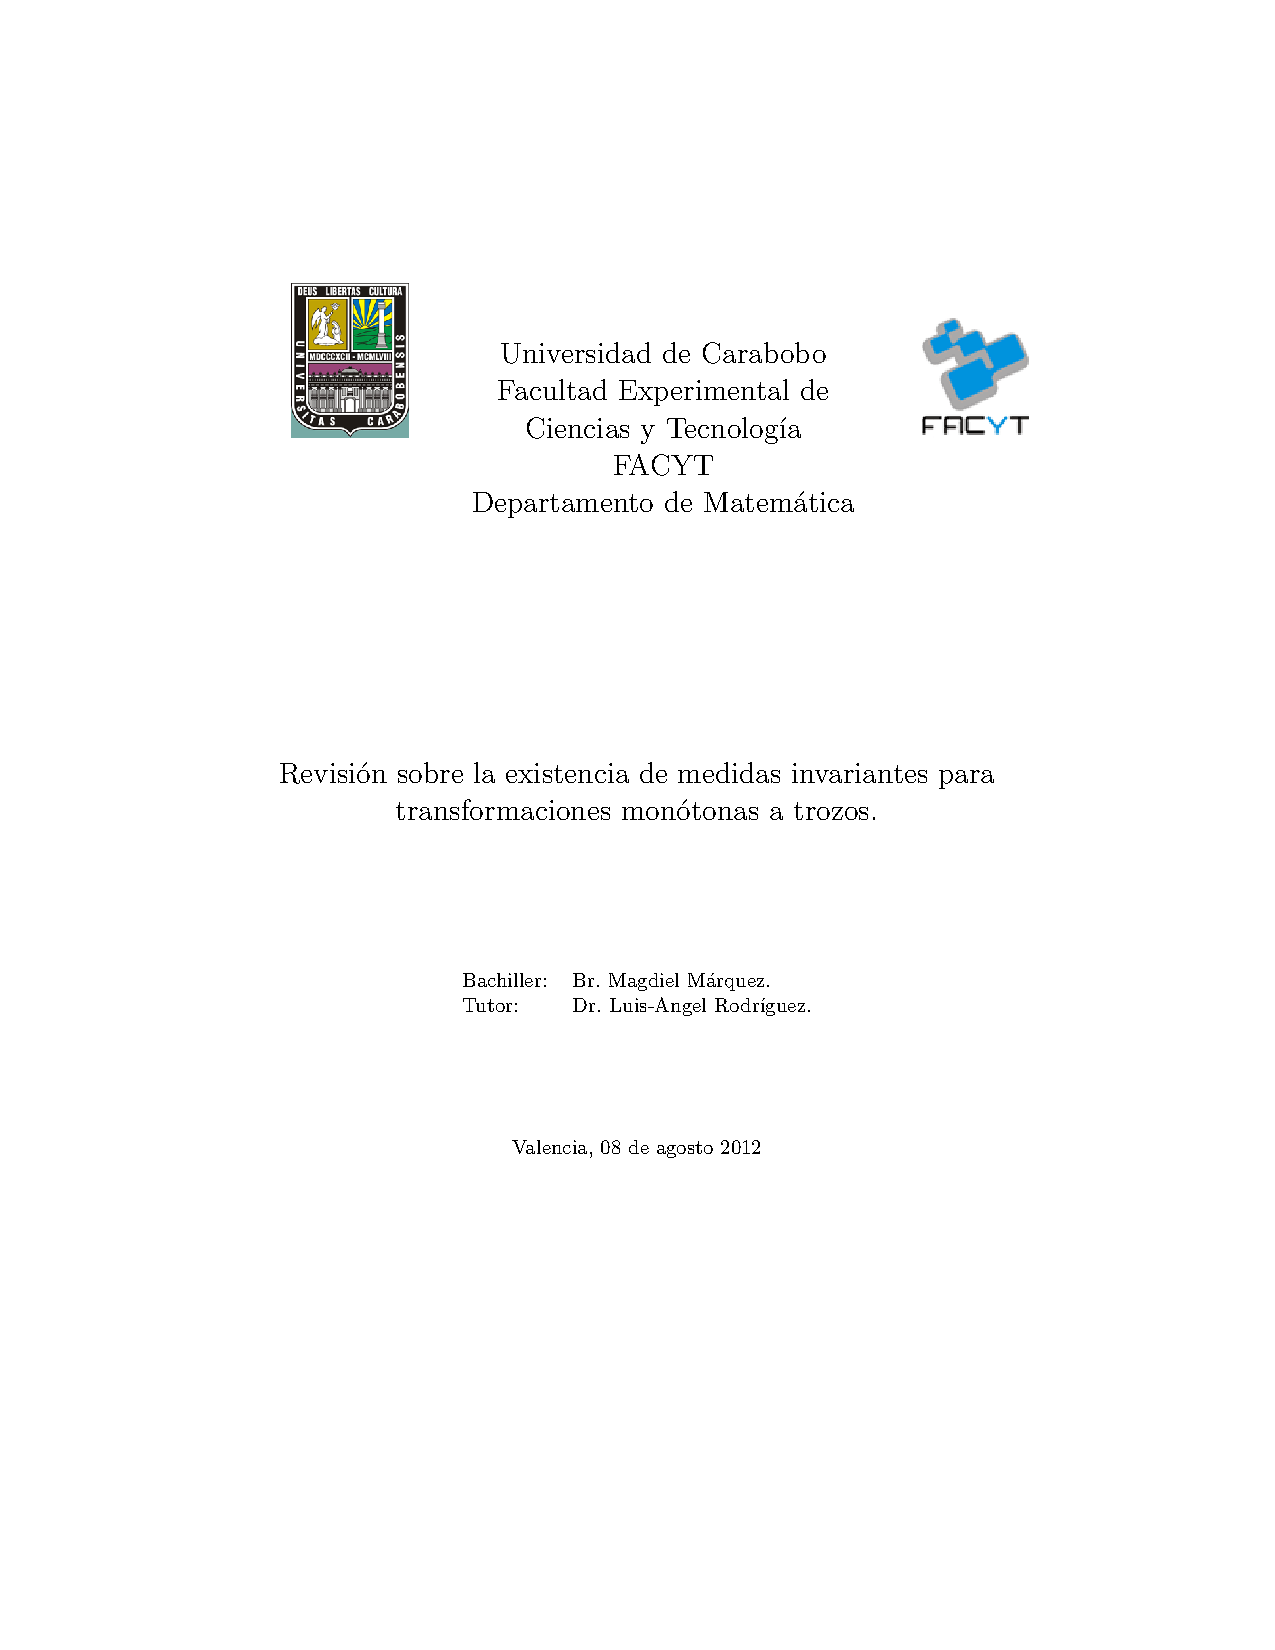
\includegraphics{graficas/tesis.6}
   \end{center}
\end{figure}
\end{ejm}

\begin{dfn}[Sitema dinamico, $(\X,\G,T)$] Sea $X$ un espacio topol�gico, $\G$ un grupo topol�gico y $(\X,\G)$ un grupo de acci�n donde $T:\X\times\G\rightarrow\X$ que cumple %~(\ref{gAccion}) y T continua.
\end{dfn}

Una �rbita es el conjunto de puntos que definen la evoluci�n de un sistema en el espacio de estados a partir de un estado inicial $x_0$.

\begin{dfn}[�rbitas de $x_0$] Sea un endomorfismo $T:X\cir$ se define los siguientes conjuntos:
    \begin{enumerate}
        \item (�rbita del futuro de $x_0$, $\Or^+(x_0)$) $\{ T^n(x_0):n\geq 0\}$
        \item (�rbita del pasado de $x_0$, $\Or^-(x_0)$) $\{ T^n(x_0):n\leq 0\}$. Si T es invertible.
        \item (�rbita de $x_0$, $\Or(x_0)$) $\{ T^n(x_0):n \in \Z \}$
    \end{enumerate}
\end{dfn}

El tipo de �rbita m�s simple son los \emph{puntos fijos} o \emph{puntos de equilibrio,} los cuales son las ra�ces del la ecuaci�n $T(x)=x$. Por otro lado se puede tener que un punto sea peri�dico despu�s de cierto tiempo, en ese caso tenemos un \emph{punto eventualmente fijo} .  El tipo de �rbita que sigue en complejidad al equilibrio es el ciclo. Un punto es c�clico o peri�dico si se aplicar� as� mismo despu�s de un tiempo $N$, al m�nimo $N$ con esta propiedad se le conoce como el per�odo. Similarmente un punto es \emph{eventualmente peri�dico} si despu�s de cierto tiempo se convierte en punto peri�dico.

\begin{dfn}[Puntos y conjuntos de inter�s] Son los puntos $p$ que cumple las siguientes condiciones:
    \begin{enumerate}
        \item (Puntos fijos) Si
            \begin{equation}
                T(p)=p \label{fijo}
            \end{equation}
        \begin{itemize}
            \item (�rbitas fijas, Fix(T)) El conjuto formado por todos los puntos fijos de T
        \end{itemize}
        \item (Puntos eventualmente fijos) Si $\exists N>0/T^n(p)=p,\forall n\geq N$.
        \item (Puntos peri�dicos) Si $\exists n>0/T^n(p)=p$. El menor entero negativo con esta propiedad se llama el \emph{per�odo primo de p}.
        \begin{itemize}
            \item (�rbitas n-peri�dicas, $Per_n(T)$) Es el conjunto formado por todas las �rbitas peri�dicas de periodo n
            \item (�rbitas periodicas, $Per(T)$) $\bigcup_{n\geq 1}{Per_n(T)}$
        \end{itemize}
        \item (Puntos eventualmente peri�dicos) Si $\exists N>0/T^N(p)$ es peri�dico.
    \end{enumerate}
\end{dfn}

Es de mayor inter�s estudiar hacen de orbitas particulares. Esto estimula la siguiente definici�n

\begin{dfn}[Conjuntos invariantes] Un conjunto $(A\subseteq\X)$ es positivamente invariante si $T(A)\subseteq A$ y negativamente invariante si $T^{-1}(A)\subseteq A$ . Un conjunto es invariante si $T(A)=A$.
\end{dfn}

\chapter{Teor�a de la Medida}

En esta secci�n expondremos las nociones b�sicas de Teor�a de la Medida que necesitaremos en los cap�tulos posteriores.
Con la intenci�n de tener un marco de referencia  en el cual se pueda apoyar las ideas a desarrollar.
En consecuencias, se comentar�n superficialmente algunos resultados de teor�a de la medida.% Para profundizar los detalles se sugiere revisar (REFERENCIAS!)


\section{Espacios Medibles y Medidas}

Hace m�s de 5000 a�os, el hombre primitivo percibe la necesidad de medir.
Interrogantes como �Qu� tan lejos? , �Qu� tan grande es?, �Cual es la capacidad? son naturales en actividad cotidianas.
De esta forma surge el manejo de longitudes, �reas y vol�menes con la necesidad de su c�lculo.
El papiro de Mosc� considerado del 1800 A.C. es uno de los documentos egipcios con problemas matem�ticos m�s antiguos que se conoce.

A Eudoxo (408 a.C. al 355 a.C.) se le atribuye la demostraci�n del volumen de un cilindro.
No obstante, es en el libro de Euclides (325 a.C. al 265 a.C) ``Los Elementos'' en que aparecen las primeras demostraciones
satisfactorias junto al m�todo cient�fico sistem�tico. No se define la longitud, �rea o volumen; se les considera
caracter�sticas que se puede medir de las figuras que define como l�nea, superficie y solido.

La palabra medir se utiliza indistintamente para estas magnitudes como para los n�meros.
Por lo que medir, para Euclides,  es un proceso de comparaci�n entre la figura y el segmento, cuadrado o cubo unitario.
Un proceso similar al usado aun actualmente en la f�sica para medir cantidades f�sicas.
En el cual se elige un patr�n \footnote{El segundo es 9,192,631,770 ciclos de radiaci�n del cesio.} y el objeto a medir se compara con este patr�n.

Arqu�medes (287 a. C. al 212 a. C.) descubri� el �rea del c�rculo mediante el m�todo de exclusi�n.
M�todo del cual se baso Newton (1642-1727) para del descubrimiento de la integral la cual permiti� el c�lculo de longitudes,
�rea o superficies curvil�neas. Descubrimiento que permite ampliar las posibilidades de objetos a medir y minimiza el
esfuerzo de su c�lculo. Observe que aunque la t�cnica de medir cambi� la medida segu�a siendo la misma.
En otras palabras, la regla se hizo el�stica o flexible para poder medir objetos de intrincado perfil pero se contin�a usando la misma regla.

\subsection{Espacios Medible}

En 1883, G. Cantor (1845-1918) proporciona la primera definici�n de medida $\mu(A)$ de un conjunto arbitrario (acotado) $A\subset\R$.
Otros autores como Stoloz en 1884 y Harnack en 1885 dan definiciones equivalentes en $\R$.Estas definiciones consideraban la
propiedad adictiva $m[A\cup B]=m[A]+m[B]$ para un par de conjuntos disjuntos.

Sin embargo, fallaban ya que en general  un conjunto y su adherencia med�a lo mismo y por tanto los racionales y los irracionales
median $1$ ambos, sobre $[0,1]$. Contradiciendo el concepto de cardinal desarrollado y propuesto por el mismo Cantor 9 a�os atr�s.
En el cual los irracionales son mayores en  cardinalidad $\aleph_1$ que la cardinalidad de los racionales $\aleph_0$.
La definici�n moderna de conjunto medible, se presenta a continuaci�n, se basa en la idea $\sigma$-algebra;
En la cual no presenta dicho inconveniente.

\begin{dfn}[$\sigma$-Algebra,$\A$] Es una familia $\A\subset\Pm(\X)$ de subconjuntos
de $\X$ que verifican las siguientes condiciones
	\begin{enumerate}
		\item $\X \in \A$
		\item Si $A\in\A$ entonces $A^c \in \A$,
		\item Si $\{A_n\}$ es una sucesi�n de conjuntos en $X$, entonces la uni�n $\cup_{n=1}^\infty\in\A$
	\end{enumerate}
	Siendo $\X$ un conjunto no vac�o.
\end{dfn}

\paragraph{Propiedades de $\sigma$-Algebra} De la definici�n se deducen las siguientes propiedades
\begin{alignat}{2}
    \X^c=\emptyset\in\A     && \text{\qquad debido a  (a) y (b)} \nonumber\\
    A\cup(\X\backslash B)=A\backslash B\in\A && \text{\qquad por (b) y (c)} \nonumber\\
    (\cap_k{(A_k)^c})^c=\cap_k{A_k}\in\A   && \text{\qquad gracias a (c) y (b)} \nonumber
\end{alignat}

\begin{dfn}[Espacio Medible, $(X,\X)$] Es el par $(X,\X)$ donde $X$ es  un conjuntos y $\X$ una $\sigma$-Algebra.
\end{dfn}

\begin{ejm} Sea $\X$ cualquier conjunto entonces $(X,\Pm (\X))$ es un espacio medible. Por otro lado $(\X,\{\X,\emptyset\})$ tambi�n es un espacio medible.
\end{ejm}

El concepto de funci�n es fundamental en la matem�tica. Este concepto nace en el an�lisis, pero se extiende en otras �reas como el Algebra, Topolog�a,  Geometr�a Diferencial entre otras. Estimuladas por la definici�n general, que no depende de entes num�ricos, aportes el trabajo de Teor�a de Conjuntos de Cantor.  Una funci�n que preserve la estructura a estudio, es un tema recurrentes en dichas �reas, lo cual trae asociadas definiciones como Homomorfismo o la Continuidad. En nuestro caso se habla de funci�n medible.

\begin{dfn}[Funci�n Medible,$f$] Si el conjunto $$f^{-1}=\{ x\in\X:f(x)\in E\}$$
pertenece a $\X$ para cada conjunto E que pertenesca a $\Y$. Siendo $f:(X,\X)\rightarrow(Y,\Y)$ una funci�n entre
un para de espacios medibles.
\end{dfn}

\begin{obs}Una funci�n $f:\X\rightarrow\R$ es medible si para cada cualquier n�meros real $\alpha$  el conjunto
$$\{ x\in\X: f(x)>\alpha\}$$
  Pertenece  $\A$
\end{obs}

\begin{figure}
    \begin{center}
        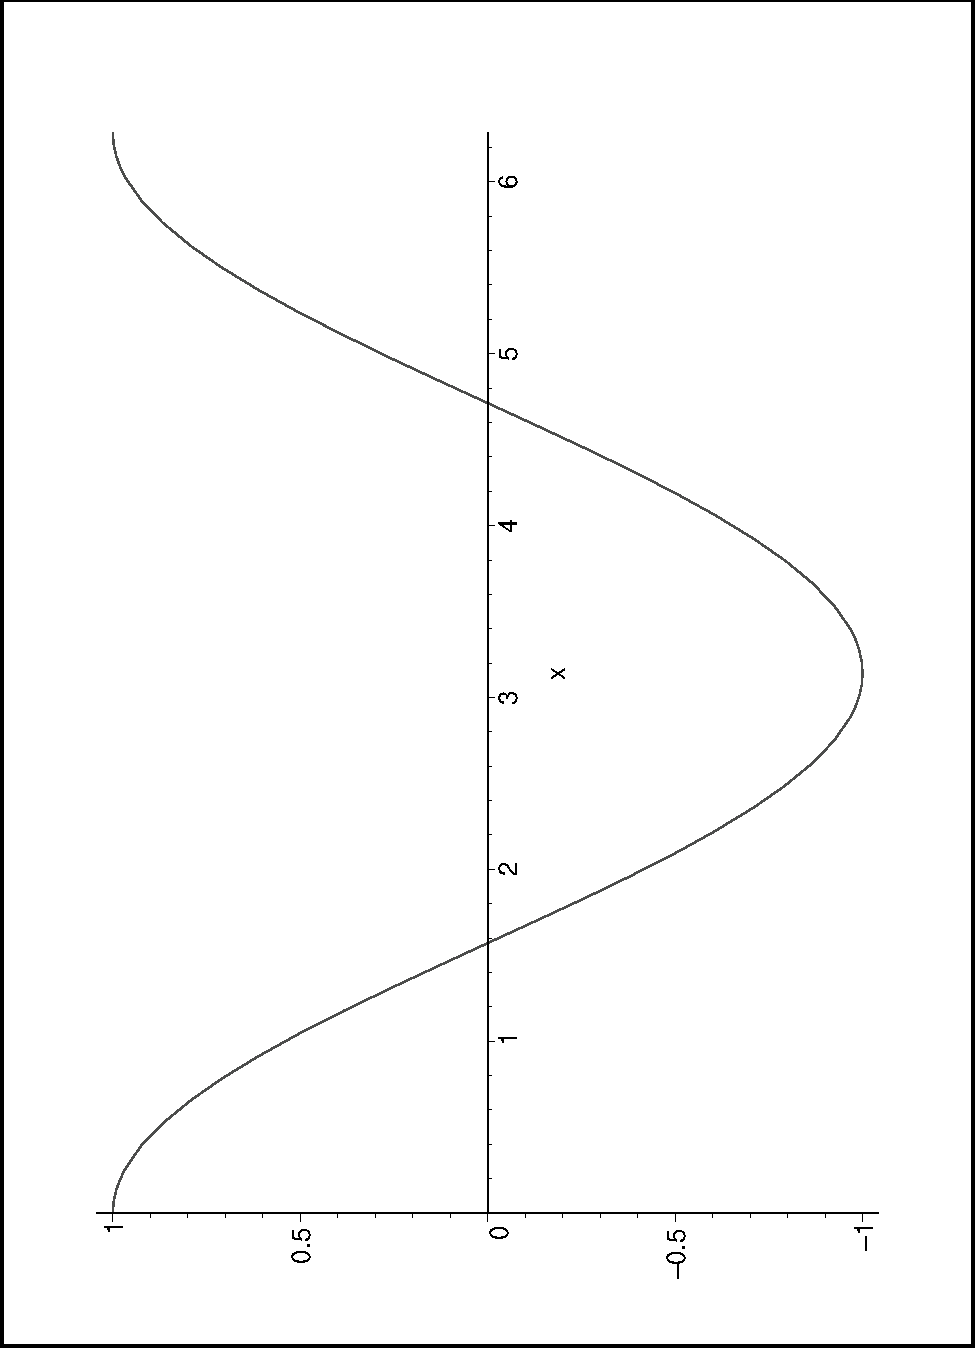
\includegraphics[angle=-90,scale=0.4]{graficas/fff}
    \end{center}
    \caption{$S(x)=4x(1-x)$\quad para $0\leq x\leq 1$. Se observa como la poblaci�n crece y decrece alrededor de $\alpha$}
\end{figure}

\begin{dfn}[Parte positiva,$f^+(x)$] Sea $f:\X\rightarrow\R$ la parte positiva es el subconjunto de funci�n definido como:
$$f^+(x)=\max{(0,f(x))}$$
\end{dfn}

\begin{figure}
    \begin{center}
        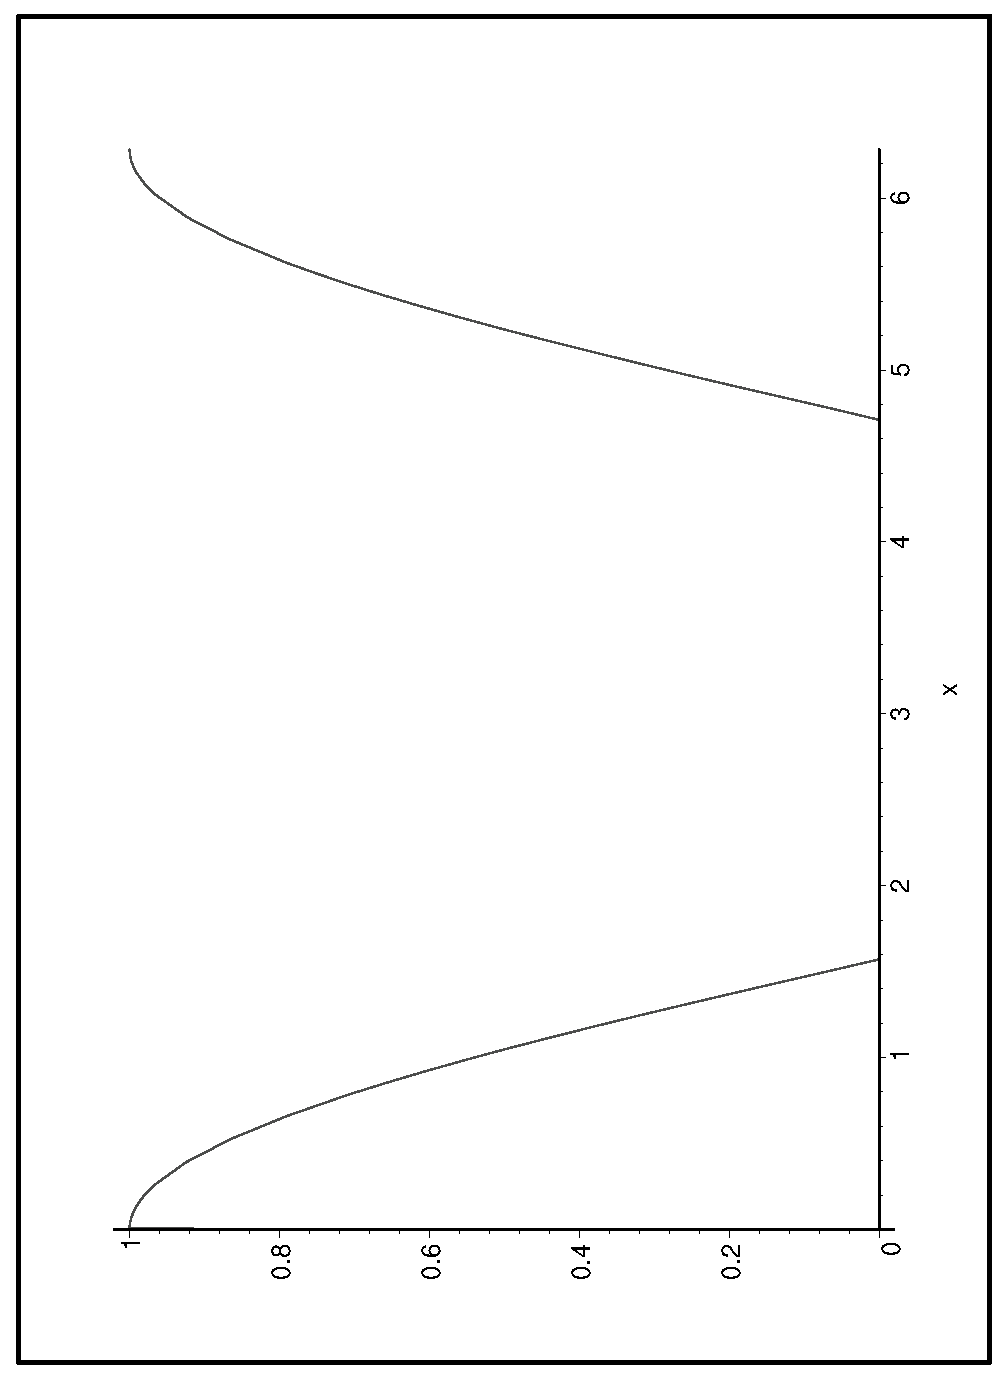
\includegraphics[angle=-90,scale=0.4]{graficas/fpo}
    \end{center}
    \caption{$S(x)=4x(1-x)$\quad para $0\leq x\leq 1$. Se observa como la poblaci�n crece y decrece alrededor de $\alpha$}
\end{figure}

\begin{dfn}[Parte negativa,$f^-(x)$] Sea $f:\X\rightarrow\R$ la parte negativa es el subconjunto de funci�n definido como:
$$f^-(x)=\max{(0,-f(x))}$$
\end{dfn}

\begin{figure}
    \begin{center}
        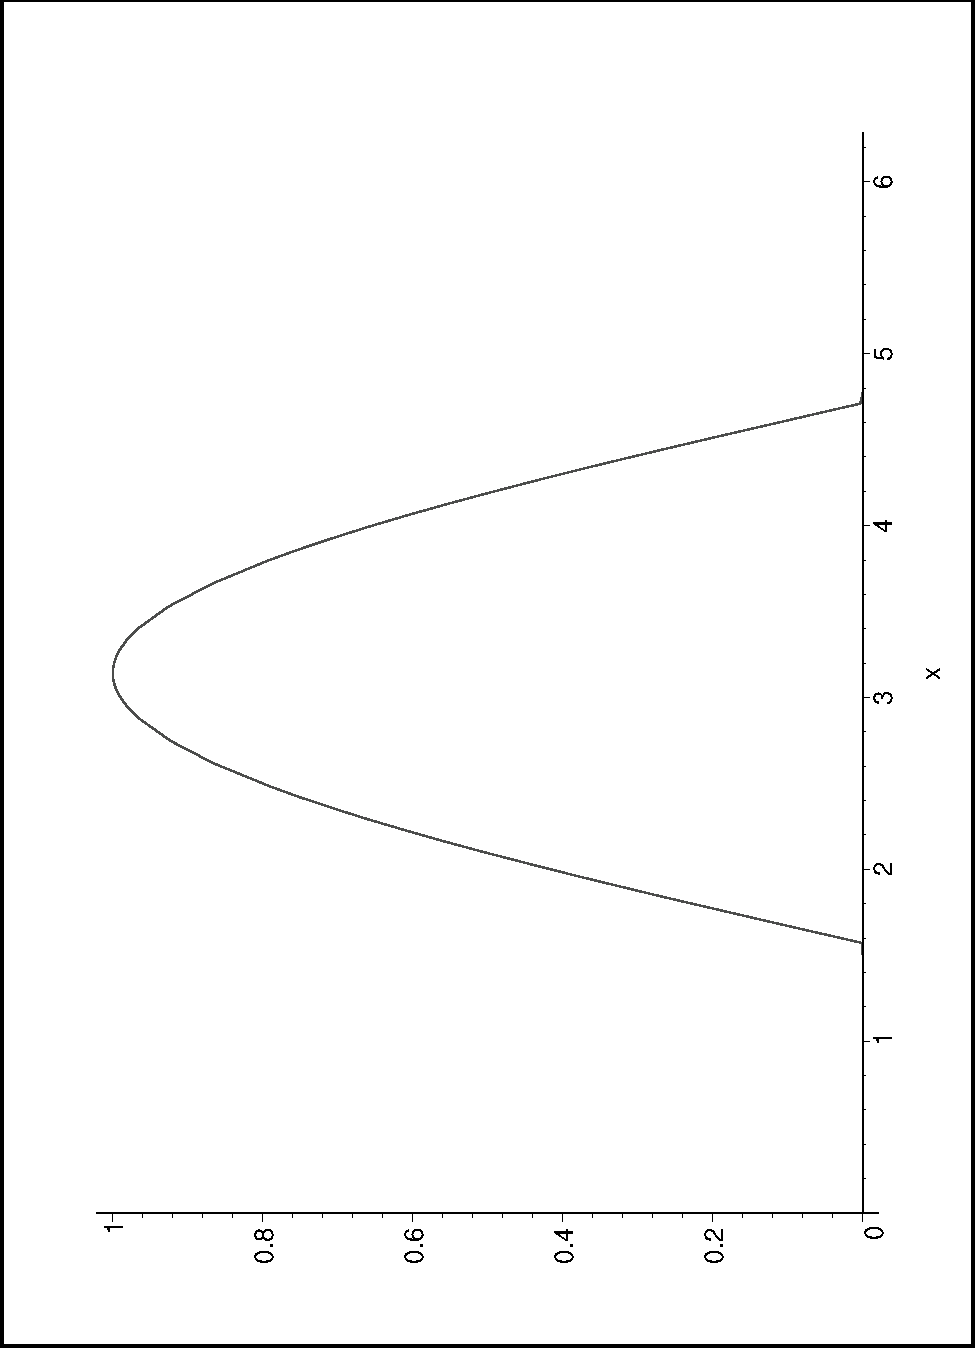
\includegraphics[angle=-90,scale=0.4]{graficas/fne}
    \end{center}
    \caption{$S(x)=4x(1-x)$\quad para $0\leq x\leq 1$. Se observa como la poblaci�n crece y decrece alrededor de $\alpha$}
\end{figure}

Apartir de las definiciones presendentes se puede deducir las siguiente propiedades

\begin{col} Para cualquier $f:\X\rightarrow\R$ se tiene
$$f(x)=f^+(x)-f^-(x)\qquad |f(x)|=f^+(x)+f^-(x)$$
\end{col}

\subsection{Espacios de Media}

Continuando con la evoluci�n historia de la medida, un tratamiento moderno fu� proporcionado por Peano (1858-1932),
el cual consider� cuando un conjunto es medible. Tomando inspiraci�n de las aproximaciones poligonales por exceso
y defecto. Defini� la medida exterior y la medida interior para definir un conjunto medible, en el caso en que ambas
medidas coinciden. Partiendo de esa definici�n probo que  la medida era aditiva; es m�s explic� la relaci�n existente
entre la medida e integraci�n. Demostrando que una funci�n acotada era Riemann integrable si y solo si el conjunto
$E$ de $\R^2$ limitado por la gr�ficas de $f$ y las rectas $x=a$, $x=b$  e $y=0$ era medible, en cuyo caso
$$\int_a^b{f(x)dx}=m[E]$$

En 1892 Jordan (1838-1922) proporciona una definici�n m�s sencilla utilizando una malla de cuadrados de igual lado,
en lugar de pol�gonos para aproximar el conjunto.  No obstante, aun se requer�a refinar la definici�n de medida debido
que en ambos casos ejemplo los racionales ya no eran medible.

Se sab�a desde la �poca de Cantor, que todo abierto $A\subset \R$ era uni�n, $A=\cup{I_n} $  a lo sumo
numerable de intervalos abiertos $I_n$ disjuntos. Partiendo de ese hecho Borel  (1871-1956) dio, en su doctorado
de 1894, el importante pas� al considerar la numerabilidad aditiva para la medida. Considerar la numerabilidad
aditiva fue un paso esencial en teor�a de la integral abstracta presentado por Lebesgue(1875-1941) en 1902. El
paso al l�mite de la integral se obtiene como consecuencia inmediata esta propiedad.
Con lo cual, se llega a la definici�n moderna de medida.

\begin{dfn}[Medida,$\mu$] Es la funci�n $\mu:\Pm(\X)\supset\A\rightarrow \R$
que cumple las siguientes propiedades:
	\begin{enumerate}
		\item $\mu(\emptyset)=0$
		\item $\mu(A)\geq 0$ para todo $A\in\A$
		\item $\mu(\bigcup_k{A_k})=\sum_k{A_k}$ donde $\{A_k\}$ es una
        sucesi�n de conjuntos disjuntos a pares
	\end{enumerate}
\end{dfn}

\paragraph{Propiedades de la Medida} Sea $E$ y $F\in \A$
\begin{alignat}{4}
    \text{Si } E\subset F && \text{ entonces } && \mu(E)\leq\mu(F) && \text{ Mon�tona} \nonumber\\
    \text{Si } \mu(E)<+\infty && \text{ entonces } &&\mu(F/E)=\mu(F)-\mu(E) && \nonumber
\end{alignat}

\begin{dfn}[Espacio Medible,$(\X,\A,\mu)$] Si $\A$ es una
$sigma$-Algebra y $\mu$ es una medida. A los conjuntos que
pertenece a $\A$ se les llama conjuntos medible.
\end{dfn}

\begin{ejm}\label{borel} Sea $\X=\R$, $\A$ son lo intervalos de $\R$ y $\mu([a,b])=|b-a|$ define un espacio medible.
 Este espacio conocido como la medida de Borel.
\end{ejm}

\begin{obs}Si $X$ e $Y$ son espacios topol�gicos $\A$, $\B$ sus respectivas $\sigma$-algebras de Borel,
entonces toda funci�n continua $f:\X\rightarrow\Y$ es medible. Ya que los Borerianos  son la menor $\sigma$-algebra
que contiene a los abiertos del espacio topol�gico. En ese caso, la definici�n de funci�n continua y funci�n medible coinciden.
\end{obs}

\begin{dfn}[Medida Finita] Si $\mu(x)<\infty$ siendo $(\X,\A,\mu)$ un espacio de medida
\end{dfn}

\begin{dfn}[Espacio de Probabilidad] Si la medida es finita y $\mu(\X)=1$
\end{dfn}

\begin{obs}Todo espacio de media finita puede ser de probabilidades. En efecto, se puede definir una medida
$$\tilde{\mu}(A)=\frac{\mu(A)}{\mu(X)} \qquad \forall A\in\A$$
Este proceso se le conoce como normalizaci�n.
\end{obs}

\begin{dfn}[Medida $\sigma$-Finita] Si la sucesi�n $\{ A_k\}$ con $A_k\in\A$ y satisface
$$X=\bigcup^\infty_{k=1}{A_k}\quad y\quad  \mu(A_k)<\infty\qquad \text{para todo k}$$
 siendo $(\X,\A,\mu)$ un espacio de medida
\end{dfn}

\begin{ejm} Sean los reales $\R$, con $\mu$ la medida de Borel es un espacio $\sigma$-finito. Debido que se puede escoger intervalos $A_k$ de la forma $[-k,k] $ con $k\in\N$, donde su uni�n numerable es $\R$ y la medida para cada $A_k$ es finita.
\end{ejm}


\begin{dfn}[Casi Seguramente, $\cs$] Si alguna propiedad se cumple en todos los subconjuntos de un espacio de medida excepto en los de medida cero.
\end{dfn}

\section{Integraci�n}

\begin{dfn}[Funci�n Simple, $\phi$] Es una funci�n a valores real $\phi:\X\rightarrow\R$ que s�lo toma un n�mero finito de valores.
\end{dfn}

\begin{dfn}[Representaci�n est�ndar] Una funci�n simple se puede representar de la siguiente forma
    $$\phi=\sum^n_{i=1}{a_i \car_{E_i}}$$
    Donde $a_j\in\R$ y $\car_{E_i}$ es una funci�n caracter�sticas de los conjuntos $E_j$.
    Los $E_i$ son subconjuntos disjuntos de $\X$ tal que $\X=\cup^n_{j=1}{E_j}$
\end{dfn}

\begin{obs}Se puede probar que la representaci�n est�ndar no depende  de los representantes, osea, de la escogencia de los $E_j$
\end{obs}

\begin{dfn}[Integral de Lebesgue, $\int_\X{f(x)\mu(dx)}$]\label{lebesgue} Se define como
    $$\int_\X{f(x)\mu(dx)}=\limi_{n\rightarrow\infty}{\int_\X{\phi_n(x)\mu(dx)}}$$
    Siendo $(\X,\A,\mu)$ un espacio de medida, $f:\X\rightarrow\R$ una funci�n acotada, arbitraria, medible, no-negativa.
     Una sucesi�n $\{ \phi_n\}$ de funciones simples que convergen uniformente a $f$.
\end{dfn}

\begin{obs} Se puede mostrar que el l�mite en la Definici�n \eqref{lebesgue}  existe y es independiente de la elecci�n de la sucesiones de funciones
    simples $\{ \phi_n \}$ que convergen uniformemente a $f$.
\end{obs}

\begin{dfn}[Integral de Lebesgue, $\int_\X{f(x)\mu(dx)}$] Se define como
    $$\int_\X{f(x)\mu(dx)}=\limi_{M\rightarrow\infty}{\int_\X{f_M(x)\mu(dx)}}$$
    Siendo $(\X,\A,\mu)$ un espacio de medida, $f:\X\rightarrow\R$ una funci�n acotada,  medible, no-negativa definida de la siguiente forma
\end{dfn}

\begin{obs} Note como $\int_\X{f(x)\mu(dx)}$ es una funci�n creciente de $M$ de modo que el l�mite en la definici�n
    siempre existe aunque podr�a ser infinito.
\end{obs}

\begin{dfn}[La integral de Lebesgue General] Se define como
 $$\int_\X{f(x)\mu(dx)}= \int_\X{f^+(x)\mu(dx)}- \int_\X{f^-(x)\mu(dx)}$$
\end{dfn}

\begin{dfn}[Funci�n Integrable] Si los t�rminos ambos
    $$\int_\X{f^+(x)\mu(dx)} \qquad \int_\X{f^-(x)\mu(dx)}$$
    Son finitos
\end{dfn}

\begin{obs} Todas las definiciones de integrales est�n definidas sobre el espacio $\X$ entero. Para $A\in\A$ se tiene, la siguiente definici�n
    $$ \int_\A{f(x)\mu(dx)}= \int_\X{f(x)\car_A(x)\mu(dx)}$$
\end{obs}

\paragraph{Propiedades de la integral de Lebesgue} Se asume $(\X,\A,\mu)$  el espacio de medida.
\begin{itemize}
    \item Si $f,g:\X\rightarrow\R$ son medible, g es integrable y $|f(x)|\leq g(x)$, entonces $f$ es integrable y
            \begin{equation}
                \Big|\int_\X{f(x)\mu(dx)}\Big|\leq\int_\X{g(x)\mu(dx)} \label{L1}
            \end{equation}
    \item Si $f$ es una funci�n medible
            \begin{equation}
                \int_\X{|f(x)|\mu(dx)}=0 si y solo si f(x)=0 \cs \label{L2}	
            \end{equation}

    \item Sea $f:\X\rightarrow\R$ una funci�n integrable y los conjuntos $A_i\in\A, \;  i=1,2,\ldots,$ disjuntos. Si $A=\cup_i{A_i}$, entonces
            \begin{equation}
                \int_\X{[\lambda_1 f_1(x)+\lambda_2 f_2(x)]\mu(dx)}=\int_\X{\lambda_1 f_1(x)\mu(dx)}+\int_\X{\lambda_2 f_2(x)\mu(dx)} \label{L3}
            \end{equation}

    \item Si $f_1,f_2: \rightarrow\R$ son funciones integrables y$\lambda_1,\lambda_2$ , entonces
          Sea  $f,g: \rightarrow\R$ son funciones medibles y una sucesi�n $f_n:\X\rightarrow\R$ de funciones medibles
          tal que $| f_n(x)|\leq g(x)$  con $f_n(x)\rightarrow f(x)\cs$. Si $g$ es integrable, entonces $f$ y $f_n$ son tambi�n integrable y
            \begin{equation}
                \limi_{n\rightarrow\infty}{\int_\X{f_n(x)\mu(dx)}}=\int_\X{f(x)\mu(dx)}
            \end{equation}
                A esta propiedad se le conoce como el Teorema de Convergencia Dominada.

    \item Sea $f:\X\rightarrow\R$ una funci�n integrable y los conjuntos $A_i\in\A$ con $i=1,2,\ldots$ disjuntos. Si $A=\cup_i{A_i}$ entonces
            \begin{equation}
                \sum_i\int_{A_i}{f(x)\mu(dx)}=\int_A{f(x)\mu(dx)}
            \end{equation}

    \item  Sea  $f: \rightarrow\R$ son funciones medibles y una sucesi�n $f_n:\X\rightarrow\R$ de funciones medibles tal que
           $0\leq f_1(x)\leq f f_2\ldots$  con $f_n(x)\rightarrow f(x)\cs$. Entonces $f$ y $f_n$ son tambi�n integrable y
            \begin{equation}
                \limi_{n\rightarrow\infty}{\int_\X{f_n(x)\mu(dx)}}=\int_\X{f(x)\mu(dx)}
            \end{equation}
            A esta propiedad se le conoce como el Teorema de Convergencia Mon�tona.
\end{itemize}

\begin{obs} Notese que $f$  es integrable si y solo si $|f|$ es integrable. Esto se puede apreciar f�cilmente viendo que $|f|=\int_\X f ^+\mu(dx)+\int_\X f^-\mu(dx)$. Si $f$ es integrable entonces $f^+$ y $f^-$ tambi�n es finito.
\end{obs}

\begin{obs} La integral de Lebesgue est� dada en varios pasos. Para cada funci�n integrable $f$ se existe una sucesi�n de funciones simples
$$f_n(x)=\sum_i{\lambda_{i,n}\car_{A_{i,n}}(x)}$$
tal que
$$\limi_{n\rightarrow\infty}{f_n}=f(x)\qquad \cs \qquad |f_n(x)|\leq |f(x)|$$
Asi, por el Teorema de Convergencia Dominada, tenemos que
$$\limi_{n\rightarrow\infty}\int_X{f_n(x)\mu(dx)}=\int_X{f(x)\mu(dx)}$$
Por lo tanto, usualmente para simplificar la prueba se verifican para funciones simples y luego se para al l�mite para extenderlo a toda las funciones.
\end{obs}

\begin{obs}La noci�n de la integral de Lebesgue es muy importante debido que solo requiere de la definici�n de un
espacio de medida $(\X,\A,\mu)$  sin la necesidad de introducir alguna otra estructura. En c�lculo la definici�n de
la integral de Riemann est� �ntimamente relacionada con propiedades algebraicas  de la recta real. Es f�cil establece
una conexi�n entre la integral de Lebesgue y la integral de Riemann. Por ejemplo, si se define $\mu$ como en el ejemplo
\ref{borel}  entonces
$$\int_{[a,b]}{f(x)\mu(dx)}=\int^b_a{f(x)dx}$$
Donde la primera es una la integral de Lebesgue y la segunda es la integral de Riemann. Esta igualdad es cierta para
cualquier funci�n $f$ Riemman integrable la cual es autom�ticamente una Lebesgue integrable. Una an�logo para dimensiones
superiores tambi�n es cierto.
\end{obs}

\section{Derivaci�n}

A partir de las propiedades de Lebesgue es f�cil probar que si $f:\X\rightarrow\R$ es una no negativa funci�n integrable
entonces $\mu_f(A)$, definido por
$$\mu_f(A)=\int_A{f(x)\mu(dx)}$$
Es una medida.De hecho, por la definici�n de la integral de Lebesgue claro que $\mu_f(A)$ es no negativo y finita,
usando la propiedad L5 es tambi�n aditiva. Adem�s,  de L2 si $\mu(A)=0$ entonces
$$\mu_f(A)=\int_A{\car_A(x)f(x)\mu(dx)}=0$$
Por lo tanto$ \car_A(x)f(x)=0\;\cs$. Asi mismo $\mu_f(A)$ satisface todas las propiedades de la medida y $\mu_f(A)=0$
donde sea $\mu(A)=0$. Cada funci�n integrable no negativa  define una medida finita puede invertirse las hip�tesis. Eso es
garantizado por el siguiente teorema.

\begin{teo}[Radon-Nikodym] Sea $(\X,\A,\R)$ un espacio de medida y sea $v$ una segunda medida finita con la propiedad que $\nu(A)$
     para todo $A\in\A$ tal que $\mu(A)=0$. Entonces existe una funci�n no negativa integrable $f:\X\rightarrow\R$ tal que
     $$\nu(A)=\int_A{f(x)\mu(dx)}\qquad \forall A\in\A$$
\end{teo}

El teorema de Radon-Nikodym ser� fundamental en el estudio del operador de Perron-Forbenius.

\begin{col} Si $(\X,\A,\mu)$ es un espacio de medida y $\nu$ es una medida finita sobre $\A$ tal que $\nu(\A)=0$
(mmmm no se) $\mu(A)=0$, entonces existe un unico elemento $f\in L^1$ tal que:
$$\nu(A)=\int_A{f(x)\mu(dx)}\qquad para \; A\in\A$$
\end{col}

\begin{dfn}[Absolutamente continua,$\mu_f$] Sea la densidad
$$\mu_f=\int {f(x)\mu(dx)} \hbox{para } A \in \A$$
donde $f\in D(\X,\A,\mu)$ . En este caso $f$ es llamada la densidad de $\mu_ f(A)$
\end{dfn}

\begin{obs}Si $f$ es integrable si y solo si |f(x) | es integrable.
\end{obs}


\section{Espacios \texorpdfstring{$L^p$}{Lp}}

\begin{dfn}[Espacios $L^p$, $L^p(\X,\A,\mu)$ o $L^p$]La familia de todas la posible funciones reales medible $f:\X\rightarrow\R$
    que satisface $$\int_\X{ | f(x)|^p\mu(dx)}<\infty$$
    Siendo $(\X,\A,\mu)$ un espacio de medida y p un n�mero real tal que $1\leq p<\infty$
\end{dfn}

\begin{obs} Si $p=1$ es habla del conjunto de todas las funciones integrables.
\end{obs}

\begin{dfn}[Norma de $f$, $|| f ||_{L^p}$]  Es el funcional
    \begin{equation}
        ||f||_{L^p}=\Big[ \int_\X{|f(x)|^p\mu(dx)}\Big]^{\frac{1}{p}}
    \end{equation}
\end{dfn}

\paragraph{Propiedades de la Norma}
    \begin{itemize}
        \item Dado $f\in L^p$
        \begin{equation}
            || f ||_{L ^p}=0\qquad \text{ si y solo si } f(x)=0\;\cs
        \end{equation}
        \item Sea $f\in L^p$ y $\alpha\in\R$
        \begin{equation}
            || \alpha f ||_{L^p}= | \alpha | \cdot ||_{L^p}f ||_{L^p}\qquad f\in L^{p}, \alpha\in\R
        \end{equation}
        \item Siendo $f,g\in L^p$
        \begin{equation}
            || f + g ||_{L^p}\leq ||  f ||_{L^p} +||g||_{L^p}\qquad f,g\in L^q
        \end{equation}
    \end{itemize}

De la propiedad L3 se deduce que $L^p$ es un espacio vectorial, ya que,
para $ f,g\in L^p$ y $\alpha\in\R$ entonces $(f+g)\in L^p$ y $\alpha f\in L^p$

\begin{dfn}[Distancia entre $f$ y $g$,$|| f + g ||_{L^p}$] Es el funcional
    $$|| f + g ||_{L^p}=\Big[\int_\X{|f(x)-g(x)|^p\mu(dx)}\Big]^{\frac{1}{p}}$$
\end{dfn}

\begin{obs} Es importante observar que el producto $fg$ de dos funciones $f,g\in L^{p}$ no es necesariamente un elemento de $L^p$
\end{obs}

\begin{dfn}[Espacio adjunto] Es $L^q(\X,\A,\mu)$ donde
    $$\Big(\frac{1}{p}\Big)+\Big(\frac{1}{q}\Big)=1$$
    Siendo $(\X,\A,\mu)$ un espacio de medida.
\end{dfn}

\begin{obs} El operador adjunto de $L_1$ es $L_\infty$, osea, las funciones medibles acotadas salvo en un conjunto de medida cero.
\end{obs}

\begin{dfn}[Producto escalar, $<f,g>$] De dos funciones de producto integrable se define como
    $$<f,g>=\int_\X{f(x)g(x)\mu(dx)}$$
siendo $f\in L^p$ y $g\in L^q$
\end{dfn}

\begin{dfn}[Inecuaci�n de  Cauchy-H�lder] Si $f\in L^{p}$ y $g\in L^{q}$ entonces
    $$|<f,g>|\leq ||f||_{L^p}  \cdot ||g||_{L^q}$$
\end{dfn}

\begin{obs}Para que la inecuaci�n tenga sentido cuando $f\in L^{1}$, $g\in L^{\infty}$, se toma para la norma
    $L^{\infty}$ la m�s peque�a constante c tal que
    $$|g(c) |\leq c$$
    Para casi todos $x\in\X$. Esta constante es llamada el supremo esencial de g. Tambi�n es una forma alternativa
    para definir las funciones de $L_{p\infty}$.
\end{obs}

\begin{obs} Se trabajar� la mayor�a de la veces en $L^1$; se indicar� en caso que la norma a usar sea contraria  a la de $L^1$.
    En otras palabras, $||f||=||f||_{L^1}$ . Observe que la desigualdad triangular en la norma $L^1$ es algunas veces una igualdad.
    Partiendo de la propiedad tenemos
    $$||f+g||=||f||+||g||\qquad f\geq 0, g\geq 0; f,g\in L^1$$
\end{obs}

Y para finalizar utilizaremos el concepto de $L^1$ para simplificar el teorema de Radon-Nikodym mostrado en el siguiente corolario 2

\begin{pro}Si $f_1$ y $f_2$ son funciones integrable tal que
$$\int_A{f_1(x)\mu(dx)}=\int_A{f_2(x)\mu(dx)}\qquad A\in\A$$
Entonces $f_1=f_2\;\cs$.
\end{pro}

\input{medida/convergencia/convergencia}






\begin{thebibliography}{a}
\bibitem{Lasota} \textsc{Lasota, A y Yorke, J.A.},
\textit{"On the existence of invariant measures for piecewise monotonic transformations"}
Trans. Amer. Math. Soc. 186 (1973) 481-486.  

\bibitem{Michael} \textsc{Lasota, A y Mackey M.C.},
\textit{"Probabilistic properties of deterministic systems"}
Cambridge University Press 1985.

\bibitem{Steve} \textsc{Papadakis S},
\textit{"The existence of absolutely continuous invariant measures for a class of piecewise monotonic transformations"}
A thesis. Concordia University 1979.
 
\end{thebibliography}
\end{document}




